\documentclass[11pt,a4paper]{article}

\usepackage[utf8]{inputenc}
\usepackage[T1,T2A]{fontenc}
\usepackage[english]{babel}
\usepackage{geometry}
\geometry{
    top=24mm,
    bottom=24mm,
    left=22mm,
    right=22mm,
    headheight=24pt,
    footskip=13mm
}

\usepackage{paratype}
\renewcommand{\familydefault}{\sfdefault}
\usepackage{amsmath,amssymb}
\usepackage{microtype}
\linespread{1.14}

\usepackage{tabularx}
\usepackage{booktabs}
\usepackage{array}
\usepackage{colortbl}
\usepackage{titlesec}
\usepackage{listings}
\usepackage{xcolor}
\usepackage{tikz}
\usetikzlibrary{shapes.geometric, arrows.meta, positioning, calc, shadows, patterns}
\usepackage[hidelinks]{hyperref}
\usepackage{bytefield}
\bytefieldsetup{
    bitformatting={\fontsize{5}{6}\selectfont\color{limmuted}},
    boxformatting={\centering\fontsize{5.2}{6.2}\selectfont}
}
\usepackage{enumitem}
\usepackage{fancyhdr}
\usepackage{lastpage}
\usepackage{tcolorbox}
\tcbuselibrary{skins,breakable,listings}

% ==============================================================================
% COLOR DESIGN CODE 60-30-10
% 60% Base (White / Light / Paper background):
%   - limwhite, limpaper, limcard, limborder, limroweven
% 30% Structural (Deep Graphite / Dark Slate):
%   - limslate, limdark, limmetal
% 10% Accent (Energetic Signal Orange):
%   - limorange, limorangeaccent, limorangelight, limorangeborder
% ==============================================================================
\definecolor{limwhite}{HTML}{FFFFFF}
\definecolor{limpaper}{HTML}{F8FAFC}
\definecolor{limcard}{HTML}{F1F5F9}
\definecolor{limborder}{HTML}{E2E8F0}
\definecolor{limborderdark}{HTML}{CBD5E1}
\definecolor{limtext}{HTML}{0F172A}
\definecolor{limmuted}{HTML}{475569}
\definecolor{limroweven}{HTML}{F8FAFC}

\definecolor{limslate}{HTML}{0F172A}
\definecolor{limdark}{HTML}{1E293B}
\definecolor{limmetal}{HTML}{334155}

\definecolor{limorange}{HTML}{FF6B00}
\definecolor{limorangeaccent}{HTML}{EA580C}
\definecolor{limorangelight}{HTML}{FFF7ED}
\definecolor{limorangeborder}{HTML}{FDBA74}
\definecolor{limamber}{HTML}{F59E0B}
\definecolor{limred}{HTML}{DC2626}
\definecolor{limredlight}{HTML}{FEF2F2}
\definecolor{limredborder}{HTML}{FECACA}
\definecolor{limreddark}{HTML}{991B1B}

% List configurations
\setlist[itemize]{leftmargin=1.5em, itemsep=3pt, topsep=4pt, label={\color{limorange}\raisebox{0.2ex}{\tiny\(\blacksquare\)}}}
\setlist[enumerate]{leftmargin=1.6em, itemsep=3pt, topsep=4pt, label={\color{limorangeaccent}\textbf{\arabic*.}}}

% Section styling
\titleformat{\section}
  {\Large\bfseries\color{limslate}}
  {\textcolor{limorange}{\rule[-2pt]{4pt}{1.3em}}\hspace{0.5em}\thesection}{0.65em}{}
  [\vspace{2mm}{\color{limorange}\rule{\linewidth}{1.2pt}}\vspace{-2mm}]

\titleformat{\subsection}
  {\large\bfseries\color{limdark}}
  {\textcolor{limorange}{\footnotesize\raisebox{0.25ex}{\(\blacktriangleright\)}}\hspace{0.45em}\thesubsection}{0.6em}{}

\titleformat{\subsubsection}
  {\normalsize\bfseries\color{limorangeaccent}}
  {\thesubsubsection}{0.5em}{}

\titlespacing*{\section}{0pt}{18pt plus 3pt minus 2pt}{10pt plus 2pt minus 2pt}
\titlespacing*{\subsection}{0pt}{14pt plus 2pt minus 2pt}{6pt plus 2pt minus 2pt}
\titlespacing*{\subsubsection}{0pt}{10pt plus 2pt minus 2pt}{4pt plus 1pt minus 1pt}

% Headers and Footers
\pagestyle{fancy}
\fancyhf{}
\fancyhead[L]{\textsf{\textbf{\textcolor{limorange}{LIM2}} \ \textcolor{limborderdark}{\textbar} \ \textcolor{limdark}{\footnotesize\nouppercase{\leftmark}}}}
\fancyhead[R]{\textsf{\textcolor{limmuted}{\footnotesize Technical Architecture Specification}}}
\renewcommand{\headrulewidth}{0.6pt}
\renewcommand{\headrule}{\hbox to\headwidth{\color{limorange}\leaders\hrule height \headrulewidth\hfill}}

\fancyfoot[L]{\textsf{\footnotesize\textcolor{limmuted}{Ivan Hniedash \textbullet\ LIM Architecture Group (Revision 2.1)}}}
\fancyfoot[R]{\textsf{\footnotesize\textcolor{limdark}{Page \textbf{\thepage} of \pageref{LastPage}}}}
\renewcommand{\footrulewidth}{0.4pt}
\renewcommand{\footrule}{\hbox to\headwidth{\color{limborder}\leaders\hrule height \footrulewidth\hfill}}

\fancypagestyle{plain}{
    \fancyhf{}
    \fancyfoot[L]{\textsf{\footnotesize\textcolor{limmuted}{Ivan Hniedash \textbullet\ LIM Architecture Group}}}
    \fancyfoot[R]{\textsf{\footnotesize\textcolor{limdark}{Page \textbf{\thepage} of \pageref{LastPage}}}}
    \renewcommand{\headrulewidth}{0pt}
    \renewcommand{\footrulewidth}{0.4pt}
    \renewcommand{\footrule}{\hbox to\headwidth{\color{limborder}\leaders\hrule height \footrulewidth\hfill}}
}

% Architecture callout boxes
\newtcolorbox{archcallout}[1][]{
    enhanced,
    breakable,
    colback=limpaper,
    colframe=limborder,
    coltitle=limdark,
    borderline west={3.5pt}{0pt}{limorange},
    sharp corners,
    rounded corners=southeast,
    arc=4pt,
    boxrule=0.8pt,
    left=12pt,
    right=12pt,
    top=8pt,
    bottom=8pt,
    fonttitle=\bfseries\sffamily,
    #1
}

\newtcolorbox{securitycallout}[1][]{
    enhanced,
    breakable,
    colback=limorangelight,
    colframe=limorangeborder,
    coltitle=limorangeaccent,
    borderline west={3.5pt}{0pt}{limorangeaccent},
    sharp corners,
    rounded corners=southeast,
    arc=4pt,
    boxrule=0.8pt,
    left=12pt,
    right=12pt,
    top=8pt,
    bottom=8pt,
    fonttitle=\bfseries\sffamily,
    #1
}

\newtcolorbox{dangerbox}[1][]{
    enhanced,
    colback=limredlight,
    colframe=limredborder,
    coltitle=limreddark,
    borderline west={3.5pt}{0pt}{limred},
    sharp corners,
    rounded corners=southeast,
    arc=4pt,
    boxrule=0.8pt,
    left=10pt,
    right=10pt,
    top=4pt,
    bottom=4pt,
    fonttitle=\bfseries\sffamily\footnotesize,
    #1
}

\newtcolorbox{statcard}[1][]{
    enhanced,
    colback=limwhite,
    colframe=limborder,
    boxrule=0.8pt,
    arc=5pt,
    width=0.315\textwidth,
    halign=center,
    valign=center,
    top=8pt,
    bottom=8pt,
    left=4pt,
    right=4pt,
    drop fuzzy shadow=gray!15,
    #1
}

% Card styles for instruction specification pages
\newtcolorbox{instructiondesc}[1][]{
    enhanced,
    breakable,
    colback=limwhite,
    colframe=limborder,
    coltitle=limdark,
    borderline west={3.5pt}{0pt}{limdark},
    arc=3pt,
    boxrule=0.8pt,
    left=10pt,right=10pt,top=7pt,bottom=7pt,
    fonttitle=\bfseries\sffamily\footnotesize,
    #1
}

\newtcolorbox{examplebox}[1][]{
    enhanced,
    breakable,
    colback=limpaper,
    colframe=limborder,
    coltitle=limorangeaccent,
    borderline west={3.5pt}{0pt}{limorange},
    arc=3pt,
    boxrule=0.8pt,
    left=10pt,right=10pt,top=7pt,bottom=7pt,
    fonttitle=\bfseries\sffamily\footnotesize,
    #1
}

% Macros for register naming
\newcommand{\reg}{\$}
\newcommand{\register}[1]{\$#1}
\newcommand{\regPTREG}{\$PTREG}
\newcommand{\regSP}{\$SP}
\newcommand{\regPC}{\$PC}
\newcommand{\regPT}{\$PT}
\newcommand{\regFREG}{\$FREG}

% Comments color in assembly listings
\definecolor{limgraycomment}{HTML}{94A3B8}

% LIM2 assembly language definition
\lstdefinelanguage{lim2asm}{
    keywords={NOP, ADD, SUB, MUL, DIV, LMR, LRM, LRR, PUSH, POP, CALL, RET, JMP, JZ, JNZ, JCR, JO, JNO, JOB, INT, INTR, CMP, AND, OR, NOT, NAND, NOR, XOR, XNOR, BSL, BSR, HALT, INC, DEC, MSP, MOD, 
              nop, add, sub, mul, div, lmr, lrm, lrr, push, pop, call, ret, jmp, jz, jnz, jcr, jo, jno, job, int, intr, cmp, and, or, not, nand, nor, xor,
              xnor, bsl, bsr, halt, inc, dec, msp, mod, ld},
    keywordstyle=\bfseries\color{limorangeaccent},
    keywords=[2]{R0, R1, R2, R3, R4, R5, R6, R7, PC, SP, PT, FREG, PTREG, 
                 PZV_VEC0_S, PZV_VEC0_E, PZV_VEC1_S, PZV_VEC1_E, PZV_VEC2_S, PZV_VEC2_E,
                 MEM_VEC_S, MEM_VEC_E, MEM_VEC_START, MEM_VEC_END,
                 INT_VEC0, INT_VEC1, INT_VEC2, INT_VEC3, INT_VEC4, INT_VEC5, INT_VEC6, INT_VEC7,
                 INT_VEC8, INT_VEC9, INT_VEC10, INT_VEC11, INT_VEC12, INT_VEC13, INT_VEC14, INT_VEC15,
                 r0, r1, r2, r3, r4, r5, r6, r7, pc, sp, pt, freg},
    keywordstyle=[2]\bfseries\color{limdark},
    sensitive=false,
    comment=[l]{;},
    commentstyle=\slshape\color{limgraycomment},
    morestring=[b]",
    morestring=[b]',
    stringstyle=\color{limslate}
}

\lstdefinestyle{lim2asmstyle}{
    language=lim2asm,
    basicstyle=\fontfamily{PTMono-TLF}\fontsize{8.5}{12}\selectfont\color{limdark},
    numbers=none,
    tabsize=4,
    showspaces=false,
    showstringspaces=false,
    breaklines=true,
    keepspaces=true,
    columns=fixed,
    basewidth=0.55em,
    extendedchars=true,
    escapeinside={(*}{*)},
    literate={\\reg0}{{\$0}}2
             {\\reg1}{{\$1}}2
             {\\reg2}{{\$2}}2
             {\\reg3}{{\$3}}2
             {\\reg4}{{\$4}}2
             {\\reg5}{{\$5}}2
             {\\reg6}{{\$6}}2
             {\\reg7}{{\$7}}2
             {\\regPTREG}{{\$PTREG}}6
             {\\regPC}{{\$PC}}3
             {\\regSP}{{\$SP}}3
             {\\regPT}{{\$PT}}3
             {\\regFREG}{{\$FREG}}5
             {\\reg}{{\$}}1
             {r0}{{\$0}}2 {r1}{{\$1}}2 {r2}{{\$2}}2 {r3}{{\$3}}2
             {r4}{{\$4}}2 {r5}{{\$5}}2 {r6}{{\$6}}2 {r7}{{\$7}}2
             {R0}{{\$0}}2 {R1}{{\$1}}2 {R2}{{\$2}}2 {R3}{{\$3}}2
             {R4}{{\$4}}2 {R5}{{\$5}}2 {R6}{{\$6}}2 {R7}{{\$7}}2
             {@0}{{\$0}}2 {@1}{{\$1}}2 {@2}{{\$2}}2 {@3}{{\$3}}2
             {@4}{{\$4}}2 {@5}{{\$5}}2 {@6}{{\$6}}2 {@7}{{\$7}}2
             {@PTREG}{{\$PTREG}}6 {@PC}{{\$PC}}3 {@SP}{{\$SP}}3
             {@PT}{{\$PT}}3 {@FREG}{{\$FREG}}5
             {\\\$0}{{\$0}}3 {\\\$1}{{\$1}}3 {\\\$2}{{\$2}}3 {\\\$3}{{\$3}}3
             {\\\$4}{{\$4}}3 {\\\$5}{{\$5}}3 {\\\$6}{{\$6}}3 {\\\$7}{{\$7}}3
             {\\\$PTREG}{{\$PTREG}}7 {\\\$PC}{{\$PC}}4 {\\\$SP}{{\$SP}}4
             {\\\$PT}{{\$PT}}4 {\\\$FREG}{{\$FREG}}6 {\\\$}{{\$}}1
             {\$0}{{\$0}}2 {\$1}{{\$1}}2 {\$2}{{\$2}}2 {\$3}{{\$3}}2
             {\$4}{{\$4}}2 {\$5}{{\$5}}2 {\$6}{{\$6}}2 {\$7}{{\$7}}2
             {\$PTREG}{{\$PTREG}}6 {\$PC}{{\$PC}}3 {\$SP}{{\$SP}}3
             {\$PT}{{\$PT}}3 {\$FREG}{{\$FREG}}5 {\$}{{\$}}1
}

% Assembly listing box
\newtcblisting{limasm}[1][]{
    enhanced,
    colback=white,
    colframe=limborder,
    boxrule=0.6pt,
    arc=2.5pt,
    left=8pt,right=8pt,top=6pt,bottom=6pt,
    listing only,
    listing engine=listings,
    listing style=lim2asmstyle,
    #1
}

% Table styling
\setlength{\tabcolsep}{7pt}
\renewcommand{\arraystretch}{1.25}

\begin{document}

% ==============================================================================
% TITLE PAGE (COVER PAGE)
% ==============================================================================
\begin{titlepage}
\hypersetup{pageanchor=false}
\begin{tikzpicture}[remember picture,overlay]
    % Top dark banner (30% structural graphite)
    \fill[limslate] (current page.north west) rectangle ([yshift=-98mm]current page.north east);
    
    % Accent orange dividing lines (10% accent)
    \fill[limorange] ([yshift=-98mm]current page.north west) rectangle ([yshift=-101mm]current page.north east);
    \fill[limorangeaccent] ([yshift=-101mm]current page.north west) rectangle ([yshift=-101.8mm]current page.north east);
    
    % Bottom structural banner
    \fill[limslate] (current page.south west) rectangle ([yshift=14mm]current page.south east);
    \fill[limorange] ([yshift=14mm]current page.south west) rectangle ([yshift=15.2mm]current page.south east);
    
    % PCB trace aesthetics
    \draw[limorange!75,line width=1.1pt] ([xshift=14mm,yshift=-18mm]current page.north west)
        -- ([xshift=48mm,yshift=-18mm]current page.north west)
        -- ([xshift=62mm,yshift=-32mm]current page.north west)
        -- ([xshift=92mm,yshift=-32mm]current page.north west);
        
    \draw[limwhite!25,line width=0.8pt] ([xshift=14mm,yshift=-28mm]current page.north west)
        -- ([xshift=38mm,yshift=-28mm]current page.north west)
        -- ([xshift=48mm,yshift=-38mm]current page.north west)
        -- ([xshift=85mm,yshift=-38mm]current page.north west);

    \draw[limorange!60,line width=0.9pt] ([xshift=14mm,yshift=-38mm]current page.north west)
        -- ([xshift=26mm,yshift=-38mm]current page.north west)
        -- ([xshift=36mm,yshift=-48mm]current page.north west)
        -- ([xshift=75mm,yshift=-48mm]current page.north west);

    \foreach \x/\y in {48/-18,62/-32,92/-32,38/-28,48/-38,85/-38,26/-38,36/-48,75/-48} {
        \fill[limorange] ([xshift=\x mm,yshift=\y mm]current page.north west) circle (1.8pt);
        \draw[limwhite!90,line width=0.5pt] ([xshift=\x mm,yshift=\y mm]current page.north west) circle (2.8pt);
    }
    
    % LIM2 chip badge
    \node[draw=limorange,fill=limdark,line width=1.4pt,rounded corners=6pt,inner sep=0pt,minimum width=26mm,minimum height=26mm] 
        at ([xshift=-32mm,yshift=-48mm]current page.north east) {
            \begin{tabular}{c}
                {\fontsize{18}{20}\selectfont\bfseries\color{limwhite}LIM2}\\[-1mm]
                {\tiny\color{limorange}\bfseries 16-BIT CORE}
            \end{tabular}
        };
\end{tikzpicture}

\vspace*{0.02\textheight}
\noindent
\begin{minipage}[t]{0.8\textwidth}
    \tcbox[
        enhanced,
        colback=limorange!20,
        colframe=limorange,
        boxrule=1pt,
        arc=3pt,
        left=8pt,right=8pt,top=3pt,bottom=3pt
    ]{%
        {\footnotesize\bfseries\color{limorange}LIM ARCHITECTURE GROUP \ \textbullet\ \ HARDWARE SPECIFICATION}%
    }
    
    \vspace{6mm}
    {\fontsize{26}{32}\selectfont\bfseries\color{limwhite}LIM2 Microprocessor Architecture\par}
    \vspace{4mm}
    {\Large\color{limwhite!90}Official Technical Reference Manual and Core Specification\par}
\end{minipage}

\vspace*{0.16\textheight}

% Quick highlights stat cards (60-30-10)
\noindent
\begin{minipage}{\textwidth}
    \centering
    \begin{statcard}
        {\large\bfseries\color{limorange}16-BIT}\\[2pt]
        {\footnotesize\bfseries\color{limdark}ALU \& Microcode}\\[2pt]
        {\footnotesize\color{limmuted}Deterministic Execution}
    \end{statcard}\hfill
    \begin{statcard}
        {\large\bfseries\color{limorange}4 GB}\\[2pt]
        {\footnotesize\bfseries\color{limdark}32-Bit Address}\\[2pt]
        {\footnotesize\color{limmuted}Linear Flat Address Space}
    \end{statcard}\hfill
    \begin{statcard}
        {\large\bfseries\color{limorange}8-BIT}\\[2pt]
        {\footnotesize\bfseries\color{limdark}External Bus}\\[2pt]
        {\footnotesize\color{limmuted}Broad Hardware Interfacing}
    \end{statcard}
\end{minipage}

\vfill

% Metadata card
\noindent
\begin{tcolorbox}[
    enhanced,
    colback=limpaper,
    colframe=limborder,
    boxrule=0.8pt,
    arc=5pt,
    left=16pt,right=16pt,top=12pt,bottom=12pt
]
    \begin{minipage}[c]{0.58\textwidth}
        {\large\bfseries\color{limdark}Technical Architecture Specification}\\[2pt]
        {\footnotesize\textcolor{limorangeaccent}{\textbf{Revision 2.1}} --- Year 2026}\\[3pt]
        {\footnotesize\color{limmuted}Status: \textbf{Active Architectural Hardware Standard}}
    \end{minipage}\hfill
    \begin{minipage}[c]{0.38\textwidth}
        \raggedleft
        {\footnotesize\color{limmuted}Lead Hardware Architect:}\\[1pt]
        {\normalsize\bfseries\color{limdark}Ivan Hniedash}\\[2pt]
        {\footnotesize\href{https://github.com/ivan365}{\color{limorange}\texttt{github.com/ivan365}}}
    \end{minipage}
\end{tcolorbox}

\vspace*{0.02\textheight}
\end{titlepage}

% ==============================================================================
% TABLE OF CONTENTS
% ==============================================================================
\hypersetup{pageanchor=true}
\pagenumbering{roman}
\tableofcontents
\clearpage
\pagenumbering{arabic}

% ==============================================================================
% SECTION 1: INTRODUCTION AND ARCHITECTURAL CONCEPT
% ==============================================================================
\section{Introduction and Architectural Concept}

\textbf{LIM2} is a 16-bit general-purpose microcoded microprocessor designed for strictly deterministic instruction execution and hardware portability. The specification does not mandate a fixed, recommended, or maximum clock frequency: it is determined entirely by the specific core implementation and the semiconductor process to which that implementation is targeted.

\subsection{Basic Principles}

\begin{archcallout}[title={Key Architectural Characteristics of LIM2}]
\begin{itemize}
    \item \textbf{8-Bit External Data Bus (\(D_0..D_7\)):} Provides direct connection to a broad range of widely available Static RAM (SRAM), ROM (EEPROM/Flash), and standard peripherals. Word and pointer assembly is handled transparently by the interface controller.
    \item \textbf{32-Bit Linear Address Bus (\(A_0..A_{31}\)):} Direct physical address space of up to 4~GB without segmentation or page-table translation overhead.
    \item \textbf{Absolute Programmer Control:} The processor hardware never performs covert background context switching, never injects hidden constants, and enforces no implicit interrupts. The CPU executes exactly and only what is explicitly programmed.
    \item \textbf{Implementation-Defined Clocking:} Operational frequencies and timing parameters are selected upon core implementation and depend on circuit topology, silicon process, and external circuitry.
    \item \textbf{Peripheral Synchronization:} When wait-state monitoring is enabled, the processor holds the current micro-operation until the \texttt{RF} line asserts High. This naturally accommodates external device latencies without constraining the core clock.
\end{itemize}
\end{archcallout}

% ==============================================================================
% SECTION 2: DATA PATH ORGANIZATION
% ==============================================================================
\section{Data Path Organization}

\subsection{Elimination of Internal Tri-State Buses}
In conventional CPU designs, functional units share a common high-impedance (High-Z) tri-state bus. In the LIM2 architecture, internal tri-state buses are entirely eliminated:
\begin{enumerate}
    \item All internal functional units are interconnected via dedicated directional digital multiplexers (MUX) and demultiplexers (DEMUX).
    \item Data flow direction is governed strictly by the active control lines of the executing micro-instruction.
    \item Operands are latched into accumulator buffer registers (\texttt{ACCB}) prior to entering the ALU, eliminating race conditions, glitches, and parasitic feedback loops.
\end{enumerate}
The detailed circuit-level schematic organization of registers, MUX/DEMUX multiplexers, and the computational data path is shown in Figure~\ref{fig:lim2_arch}.

\subsection{Microcode Control}
Each LIM2 assembly instruction is expanded by the control unit into a fixed sequence of chip-level micro-operations:
\begin{itemize}
    \item Switching the register file multiplexer selectors;
    \item Configuring the ALU operation mode (\(+\), \(-\), \(\times\), \(/\), bitwise logic operations, shifts);
    \item Synchronizing memory read/write cycles with the external bus interface.
\end{itemize}
Instruction execution is strictly sequential: the next instruction is not fetched from memory until the microprogram of the current instruction has fully completed its execution cycle.

\begin{figure}[htbp]
\centering
\begin{tcolorbox}[
    enhanced,
    colback=limwhite,
    colframe=limborder,
    boxrule=0.6pt,
    arc=4pt,
    left=6pt,right=6pt,top=6pt,bottom=6pt,
    drop fuzzy shadow=gray!12
]
    \centering
    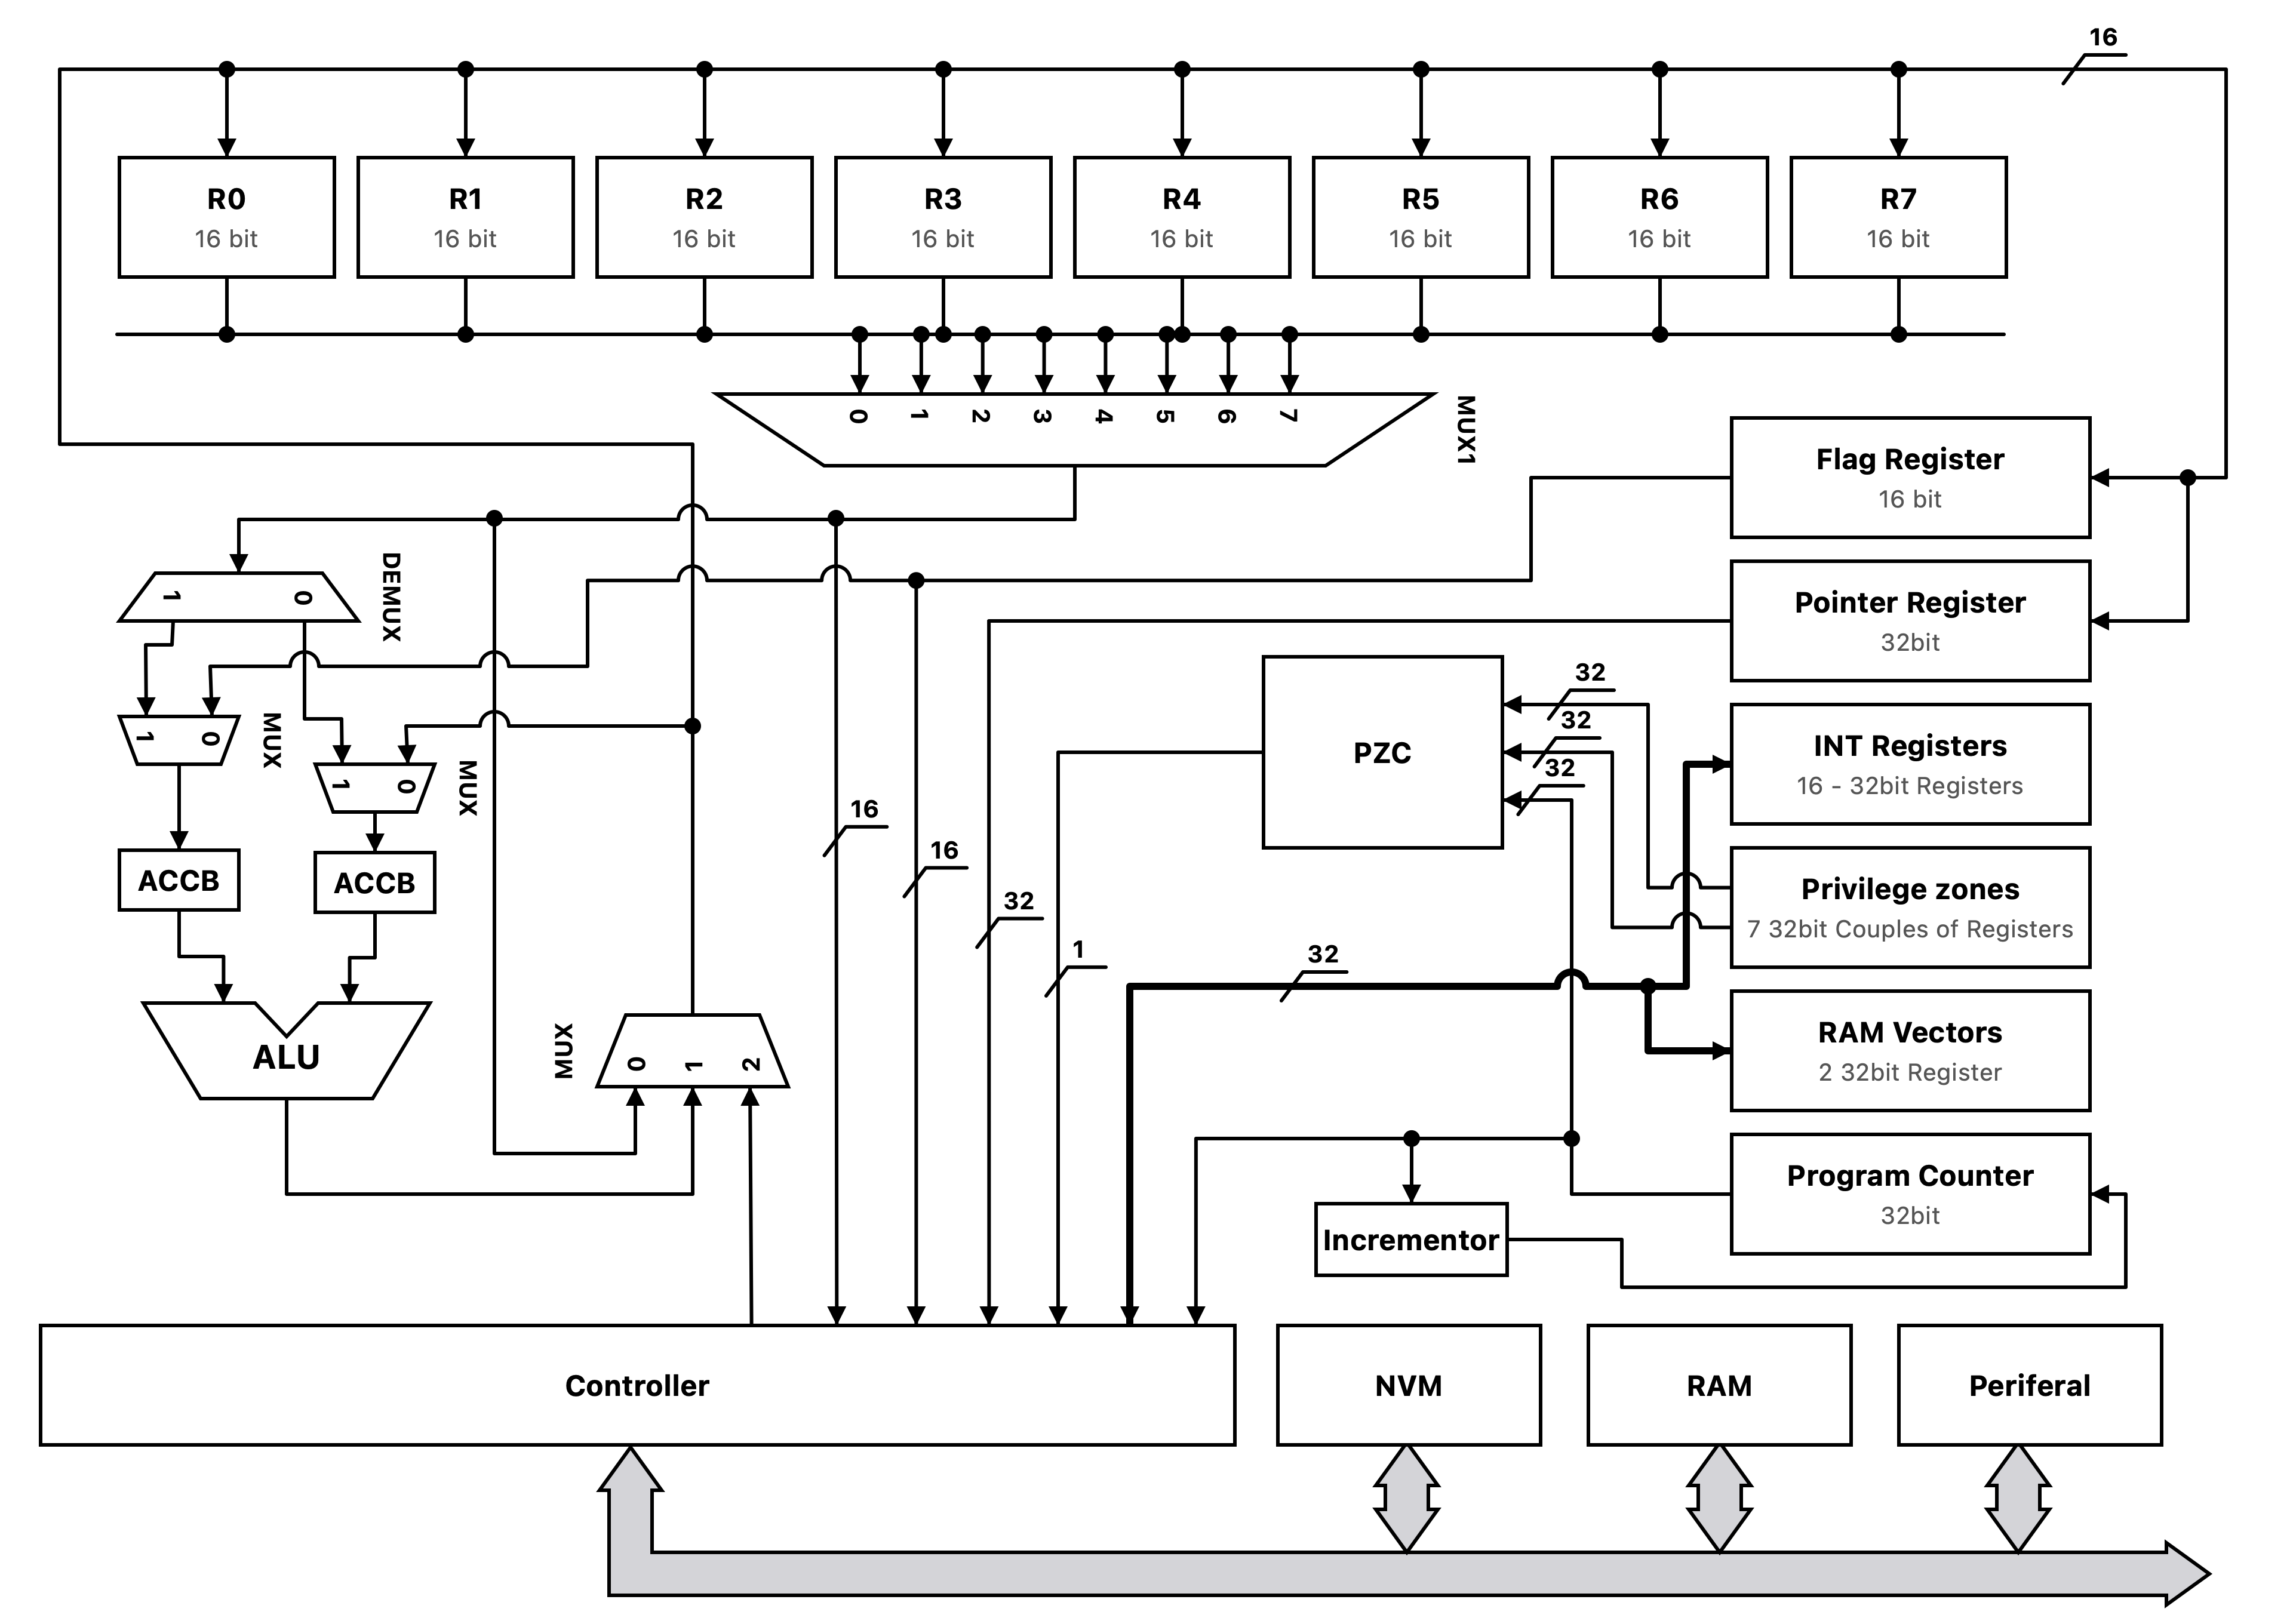
\includegraphics[width=\linewidth]{images/lim2.png}
\end{tcolorbox}
\vspace{-2mm}
\caption{\textbf{LIM2 Microarchitectural Block Diagram:} Organization of register files R0--R7, directional MUX/DEMUX buses, ACCB latch buffers, ALU execution unit, Privilege Zone Controller (PZC), and system bus interface}
\label{fig:lim2_arch}
\end{figure}

% ==============================================================================
% SECTION 3: REGISTER MODEL
% ==============================================================================
\section{Register Model and System Cell Architecture}

The LIM M2 microarchitecture utilizes a strictly quantized, orthogonal register model partitioned into general-purpose registers, arithmetic accumulators, hardware execution pointers, and an indexed 8-bit space of 256 quantized 16-bit system cells (\texttt{REG\_ID} \(0\)--\(255\)).

\subsection{Architectural Register Summary}

\noindent
\begin{minipage}{\textwidth}
\centering
\small
\begin{tabularx}{\textwidth}{l c c l X}
\toprule
\rowcolor{limslate}
\textcolor{white}{\textbf{Register}} & \textcolor{white}{\textbf{Bits}} & \textcolor{white}{\textbf{Reset}} & \textcolor{white}{\textbf{Type}} & \textcolor{white}{\textbf{Microarchitectural Role}} \\
\midrule
\rowcolors{2}{limroweven}{white}
\textbf{R0 -- R7} & 16 & \texttt{0x0000} & General Purpose & Primary registers for ALU, logic, shift, and memory operands. \\
\textbf{ACCA} & 16 & \texttt{0x0000} & ALU Latch A & Internal ALU operand A buffer; holds intermediate computation state. \\
\textbf{ACCB} & 16 & \texttt{0x0000} & ALU Latch B & Internal ALU operand B buffer; feeds second operand to execution units. \\
\textbf{PC} & 32 & \texttt{0x00000000} & Instruction Ptr & Linear 32-bit physical Program Counter (up to 4~GB address space). \\
\textbf{SP (SREG)} & 32 & \texttt{0x00000000} & Stack Pointer & Hardware stack pointer for subroutine calls, interrupts, and push/pop. \\
\textbf{PT (PTREG)} & 32 & \texttt{0x00000000} & Base Pointer & Streaming memory pointer with automatic post-increment (\texttt{AIP}). \\
\textbf{FREG} & 16 & \texttt{0x1800} & Status \& Control & Condition codes, ALU flags, interrupt enable (\texttt{MIE}), privilege (\texttt{PRV}). \\
\bottomrule
\end{tabularx}
\end{minipage}

\vspace{3mm}

\subsection{Quantized 16-bit System Register Cells (REG\_ID 0--255)}

All privileged and configuration registers are addressed via the \texttt{MSP} instruction as quantized 16-bit cells. A full 8-bit address space (\texttt{REG\_ID} \(0\)--\(255\)) is allocated. Registers wider than 16 bits are structured as consecutive pairs: the lower cell index represents the lower 16 bits (\texttt{\_lo}), while the higher cell index represents the upper 16 bits (\texttt{\_hi}). Both clean identifiers (\texttt{freg}, \texttt{sp}, \texttt{ir0}) and prefixed versions (\texttt{\$freg}, \texttt{\$sp}, \texttt{\$ir0}) are recognized interchangeably by the assembler.

\vspace{1.5mm}
\noindent\textbf{Table 3.1: Interrupt Vector Table (IVT) Cells (Cells 0--31, IRQ0--IRQ15)}
\par\vspace{1mm}\noindent
{\footnotesize
\renewcommand{\arraystretch}{0.93}
\begin{tabularx}{\textwidth}{@{} l c c l >{\raggedright\arraybackslash}X @{}}
\toprule
\rowcolor{limslate}
\textcolor{white}{\textbf{Vector}} & \textcolor{white}{\textbf{Dec Cells}} & \textcolor{white}{\textbf{Hex Cells}} & \textcolor{white}{\textbf{Cell Aliases (Lo, Hi)}} & \textcolor{white}{\textbf{Functional Description and Handler Purpose}} \\
\midrule
\rowcolors{2}{limroweven}{white}
\textbf{IRQ 0} (\texttt{ir0}) & 0, 1 & \texttt{0x00, 0x01} & \texttt{ir0\_lo, ir0\_hi} & Core Reset entry and Hardware Timer 0 ISR vector. \\
\textbf{IRQ 1} (\texttt{ir1}) & 2, 3 & \texttt{0x02, 0x03} & \texttt{ir1\_lo, ir1\_hi} & Arithmetic Error Trap (division by zero / \texttt{EM=1}). \\
\textbf{IRQ 2} (\texttt{ir2}) & 4, 5 & \texttt{0x04, 0x05} & \texttt{ir2\_lo, ir2\_hi} & System Call Trap (Syscall service entry via \texttt{INT 2}). \\
\textbf{IRQ 3} (\texttt{ir3}) & 6, 7 & \texttt{0x06, 0x07} & \texttt{ir3\_lo, ir3\_hi} & External Peripheral Interrupt 3 (UART / Terminal console). \\
\textbf{IRQ 4} (\texttt{ir4}) & 8, 9 & \texttt{0x08, 0x09} & \texttt{ir4\_lo, ir4\_hi} & Hardware Peripheral Interrupt 4 (General I/O controller). \\
\textbf{IRQ 5} (\texttt{ir5}) & 10, 11 & \texttt{0x0A, 0x0B} & \texttt{ir5\_lo, ir5\_hi} & Hardware Peripheral Interrupt 5 (Storage / Disk controller). \\
\textbf{IRQ 6} (\texttt{ir6}) & 12, 13 & \texttt{0x0C, 0x0D} & \texttt{ir6\_lo, ir6\_hi} & Hardware Peripheral Interrupt 6 (Network / Expansion bus). \\
\textbf{IRQ 7} (\texttt{ir7}) & 14, 15 & \texttt{0x0E, 0x0F} & \texttt{ir7\_lo, ir7\_hi} & Hardware Peripheral Interrupt 7 (Real-time clock / periodic tick). \\
\textbf{IRQ 8--11} & 16--23 & \texttt{0x10--0x17} & \texttt{ir8\_lo}..\texttt{ir11\_hi} & Software and User Interrupt Vectors 8 through 11 (even: \texttt{\_lo}, odd: \texttt{\_hi}). \\
\textbf{IRQ 12--15} & 24--31 & \texttt{0x18--0x1F} & \texttt{ir12\_lo}..\texttt{ir15\_hi} & Dedicated Core Hardware Timers 1--4 (12: T1, 13: T2, 14: T3, 15: T4). \\
\bottomrule
\end{tabularx}
}
\par\vspace{1.5mm}\noindent{\scriptsize\textit{Note: Compact aliases \texttt{iv0l}..\texttt{iv15h} are also accepted. Composite 32-bit identifiers \texttt{ir0}..\texttt{ir15} expand into low and high cell pairs.}}\par

\clearpage

\noindent\textbf{Table 3.2: Privilege Protection Zones and Physical RAM Boundaries (Cells 32--63)}
\par\vspace{1.5mm}\noindent
{\footnotesize
\renewcommand{\arraystretch}{0.93}
\begin{tabularx}{\textwidth}{@{} l c c l >{\raggedright\arraybackslash}X @{}}
\toprule
\rowcolor{limslate}
\textcolor{white}{\textbf{Zone / Vector}} & \textcolor{white}{\textbf{Dec Cells}} & \textcolor{white}{\textbf{Hex Cells}} & \textcolor{white}{\textbf{Boundary Aliases (Start / End)}} & \textcolor{white}{\textbf{Security Rules and Memory Isolation Window}} \\
\midrule
\rowcolors{2}{limroweven}{white}
\textbf{Zone 0} (\texttt{pz0}) & 32--35 & \texttt{0x20--0x23} & \texttt{pz0\_start} / \texttt{pz0\_end} & Privilege Zone 0 window. In User Mode (\(\texttt{PRV}=0\)), writes to cells 32--59 blocked outside this window. \\
\textbf{Zone 1} (\texttt{pz1}) & 36--39 & \texttt{0x24--0x27} & \texttt{pz1\_start} / \texttt{pz1\_end} & Privilege Zone 1 window. Core kernel and supervisor code/data region. \\
\textbf{Zone 2} (\texttt{pz2}) & 40--43 & \texttt{0x28--0x2B} & \texttt{pz2\_start} / \texttt{pz2\_end} & Privilege Zone 2 window. Privileged device drivers and memory manager. \\
\textbf{Zone 3} (\texttt{pz3}) & 44--47 & \texttt{0x2C--0x2F} & \texttt{pz3\_start} / \texttt{pz3\_end} & Privilege Zone 3 window. Operating system shared services and IPC. \\
\textbf{Zone 4} (\texttt{pz4}) & 48--51 & \texttt{0x30--0x33} & \texttt{pz4\_start} / \texttt{pz4\_end} & Privilege Zone 4 window. Task isolation boundary. \\
\textbf{Zone 5} (\texttt{pz5}) & 52--55 & \texttt{0x34--0x37} & \texttt{pz5\_start} / \texttt{pz5\_end} & Privilege Zone 5 window. Task isolation boundary. \\
\textbf{Zone 6} (\texttt{pz6}) & 56--59 & \texttt{0x38--0x3B} & \texttt{pz6\_start} / \texttt{pz6\_end} & Privilege Zone 6 window. Task isolation boundary. \\
\textbf{RAM Base} & 60, 61 & \texttt{0x3C, 0x3D} & \texttt{ram\_base} & User RAM Physical Base (default: \texttt{0x00000000}). Unrestricted across all modes. \\
\textbf{RAM Limit} & 62, 63 & \texttt{0x3E, 0x3F} & \texttt{ram\_limit} & User RAM Physical Upper Limit (highest allowable physical RAM byte address). \\
\bottomrule
\end{tabularx}
}
\par\vspace{1.5mm}\noindent{\scriptsize\textit{Note: Individual 16-bit boundaries are accessible via \texttt{\_lo}/\texttt{\_hi} (e.g. \texttt{pz0\_start\_lo}) or compact aliases \texttt{pz0sl, pz0sh} / \texttt{pz0el, pz0eh}. RAM bounds support \texttt{ram\_bl, ram\_bh} / \texttt{ram\_ll, ram\_lh}.}}\par

\clearpage

\noindent\textbf{Table 3.3: Control Registers, Hardware Timers, and System Extensions (Cells 64--255)}
\par\vspace{1.5mm}\noindent
{\footnotesize
\renewcommand{\arraystretch}{0.90}
\begin{tabularx}{\textwidth}{@{} l c c l >{\raggedright\arraybackslash}X @{}}
\toprule
\rowcolor{limslate}
\textcolor{white}{\textbf{Register}} & \textcolor{white}{\textbf{Dec Cells}} & \textcolor{white}{\textbf{Hex Cells}} & \textcolor{white}{\textbf{Mnemonics and Aliases}} & \textcolor{white}{\textbf{Functional Description and Microcode Usage}} \\
\midrule
\rowcolors{2}{limroweven}{white}
\textbf{T1\_CNT} & 64, 65 & \texttt{0x40, 0x41} & \texttt{t1\_cnt} (\texttt{t1\_cnt\_lo, hi}) & 32-bit Up-counter for Timer 1. Increments every clock cycle. \\
\textbf{T1\_MATCH} & 66, 67 & \texttt{0x42, 0x43} & \texttt{t1\_match} (\texttt{t1\_match\_lo, hi}) & 32-bit Comparator match threshold. Triggers IRQ 12 and resets \texttt{t1\_cnt}. \\
\textbf{T1\_TIME} & 68, 69 & \texttt{0x44, 0x45} & \texttt{t1\_time} (\texttt{t1\_time\_lo, hi}) & 32-bit Elapsed time accumulator (increments upon each T1 match event). \\
\textbf{T2\_CNT} & 70, 71 & \texttt{0x46, 0x47} & \texttt{t2\_cnt} (\texttt{t2\_cnt\_lo, hi}) & 32-bit Periodic Down-counter for Timer 2. Decrements every cycle. \\
\textbf{T2\_RELOAD} & 72, 73 & \texttt{0x48, 0x49} & \texttt{t2\_reload} (\texttt{t2\_reload\_lo, hi}) & 32-bit Periodic reload period. Triggers IRQ 13 and reloads at zero. \\
\textbf{T3\_CNT} & 74, 75 & \texttt{0x4A, 0x4B} & \texttt{t3\_cnt} (\texttt{t3\_cnt\_lo, hi}) & 32-bit One-shot Down-counter. Stops and triggers IRQ 14 upon zero. \\
\textbf{T4\_CNT} & 76 & \texttt{0x4C} & \texttt{t4\_cnt} & 16-bit Instruction Quantum Down-counter (decrements per instruction). \\
\textbf{T4\_RELOAD} & 77 & \texttt{0x4D} & \texttt{t4\_reload} & 16-bit Instruction quantum reload period. Triggers IRQ 15 at zero. \\
\textbf{TSR} & 78 & \texttt{0x4E} & \texttt{tsr} (\texttt{timer\_ctrl}) & 16-bit Timer Setting Register: enables (15:12), IRQ masks (11:8), status (7:4). \\
\textbf{Reserved} & 79--127 & \texttt{0x4F--0x7F} & --- & 49 Reserved cells for future core extensions and MMU tables. \\
\textbf{FREG} & 128 & \texttt{0x80} & \texttt{freg} (\texttt{flags}, \texttt{sr}) & 16-bit Status and Control Flags: \texttt{ZF, CF, OF, EM, CMP, CLK, SSRC, MIE, DWR, PRV, AIP, DBIT, SMOD, INTR}. \\
\textbf{SP (SREG)} & 129, 130 & \texttt{0x81, 0x82} & \texttt{sp} (\texttt{sp\_lo, sp\_hi}, \texttt{spl, sph}) & 32-bit Hardware Stack Pointer. Cell 129: \texttt{SP[15:0]} (\texttt{\_lo}), Cell 130: \texttt{SP[31:16]} (\texttt{\_hi}). \\
\textbf{PT (PTREG)} & 131, 132 & \texttt{0x83, 0x84} & \texttt{ptreg} (\texttt{ptreg\_lo, ptreg\_hi}, \texttt{ptl, pth}) & 32-bit Streaming Base Pointer. Cell 131: \texttt{PT[15:0]} (\texttt{\_lo}), Cell 132: \texttt{PT[31:16]} (\texttt{\_hi}). Auto-incremented if \texttt{AIP=1}. \\
\textbf{Reserved} & 133--255 & \texttt{0x85--0xFF} & --- & 123 Reserved cells for hardware peripherals. \\
\bottomrule
\end{tabularx}
}

\vspace{3mm}

\subsection{Composite 32-bit Vector Register Aliases}
To maximize programmer convenience, the LIM M2 assembler transparently recognizes 32-bit register identifiers (with or without \texttt{\$}) and expands single \texttt{MSP.ld} instructions into sequential 16-bit operations:
\begin{equation*}
    \text{\texttt{MSP.ld sp, 0x0007FFFC}} \quad \Longrightarrow \quad
    \begin{cases}
        \text{\texttt{MSP.ld sp\_lo, 0xFFFC}} & (\text{Cell } 129, \text{Low 16 bits}) \\
        \text{\texttt{MSP.ld sp\_hi, 0x0007}} & (\text{Cell } 130, \text{High 16 bits})
    \end{cases}
\end{equation*}
Supported composite identifiers include:
\begin{itemize}[leftmargin=10pt,itemsep=1pt]
    \item \textbf{\texttt{sp} / \texttt{sreg}:} 32-bit Hardware Stack Pointer (Cells 129 and 130).
    \item \textbf{\texttt{ptreg} / \texttt{pt}:} 32-bit Base Pointer (Cells 131 and 132).
    \item \textbf{\texttt{ir0} -- \texttt{ir15}:} 16 Interrupt Vectors IR0--IR15 (Cells \(2k\) and \(2k+1\)).
    \item \textbf{\texttt{pz0\_start} -- \texttt{pz6\_end} (\texttt{pv0} -- \texttt{pv13}):} 7 Privilege Zone boundary pairs.
    \item \textbf{\texttt{ram\_base} / \texttt{ram\_limit}:} Physical RAM boundaries (Cells 60/61 and 62/63).
    \item \textbf{\texttt{t1\_cnt}, \texttt{t1\_match}, \texttt{t1\_time}:} 32-bit Timer 1 counters and comparator (Cells 64/65, 66/67, 68/69).
    \item \textbf{\texttt{t2\_cnt}, \texttt{t2\_reload}:} 32-bit Timer 2 counter and periodic reload threshold (Cells 70/71, 72/73).
    \item \textbf{\texttt{t3\_cnt}:} 32-bit Timer 3 one-shot down-counter (Cells 74/75).
\end{itemize}

% ==============================================================================
% SECTION 4: FLAGS AND CONTROL REGISTER (FREG, 16-BIT)
% ==============================================================================
\section{Flags and Control Register (FREG, 16-bit)}

The \texttt{FREG} register combines arithmetic condition flags, clocking configuration bits, interrupt enables, and core privilege mode.

\vspace{2mm}
\noindent
\begin{minipage}{\textwidth}
\centering
\begin{bytefield}[bitwidth=2.15em, endianness=big]{16}
    \bitheader{15,14,13,12,11,10,9,8,7,6,5,4,3,2,1,0} \\
    \bitbox{1}{\fontsize{4.5}{5.2}\selectfont\textbf{INTR}} &
    \bitbox{1}{\fontsize{4.5}{5.2}\selectfont\textbf{SMOD}} &
    \bitbox{1}{\fontsize{4.5}{5.2}\selectfont\textbf{DBIT}} &
    \bitbox{1}{\fontsize{4.5}{5.2}\selectfont\textbf{AIP}} &
    \bitbox{1}{\fontsize{4.5}{5.2}\selectfont\textbf{PRV}} &
    \bitbox{1}{\fontsize{4.5}{5.2}\selectfont\textbf{DWR}} &
    \bitbox{1}{\fontsize{4.5}{5.2}\selectfont\textbf{MIE}} &
    \bitbox{1}{\fontsize{4.5}{5.2}\selectfont\textbf{SSRC}} &
    \bitbox{2}{\fontsize{5.5}{6.5}\selectfont\textbf{CLK}} &
    \bitbox{2}{\fontsize{5.5}{6.5}\selectfont\textbf{CMP}} &
    \bitbox{1}{\fontsize{4.5}{5.2}\selectfont\textbf{EM}} &
    \bitbox{1}{\fontsize{4.5}{5.2}\selectfont\textbf{OF}} &
    \bitbox{1}{\fontsize{4.5}{5.2}\selectfont\textbf{CF}} &
    \bitbox{1}{\fontsize{4.5}{5.2}\selectfont\textbf{ZF}}
\end{bytefield}
\end{minipage}
\vspace{3mm}

\noindent\textbf{Table 4.1: Bit Definition Map of Flags and Control Register (FREG)}
\par\vspace{1.5mm}\noindent
{\small
\begin{tabularx}{\textwidth}{c c l X}
\toprule
\rowcolor{limslate}
\textcolor{white}{\textbf{Bit}} & \textcolor{white}{\textbf{Flag}} & \textcolor{white}{\textbf{Name}} & \textcolor{white}{\textbf{Functional Description}} \\
\midrule
\rowcolors{2}{limroweven}{white}
0 & \textbf{\texttt{ZF}} & Zero Flag & Set to 1 if the operation result equals zero. \\
1 & \textbf{\texttt{CF}} & Carry Flag & Carry / borrow flag in arithmetic operations. \\
2 & \textbf{\texttt{OF}} & Overflow Flag & Two's complement signed overflow indicator. \\
3 & \textbf{\texttt{EM}} & Error Math & Hardware latch for divide-by-zero and arithmetic faults. \\
4--5 & \textbf{\texttt{CMP}} & Compare Result & Comparator status: \texttt{00} = no comparison, \texttt{01} = \(<\), \texttt{10} = \(=\), \texttt{11} = \(>\). \\
6--7 & \textbf{\texttt{CLK}} & Clock Mode & Clock mode or prescaler configuration; frequencies depend on core implementation. \\
8 & \textbf{\texttt{SSRC}} & Shift Source & Inflow bit source during linear shift (\texttt{SMOD=0}): 0 = zero, 1 = bit from \texttt{DBIT}. \\
9 & \textbf{\texttt{MIE}} & Master Int Enable & External maskable interrupt enable. Software and internal faults remain active unconditionally. \\
10 & \textbf{\texttt{DWR}} & Disable Wait Ready & When 0, CPU pauses microcode waiting for \texttt{RF} pin. When 1, wait state is disabled. \\
11 & \textbf{\texttt{PRV}} & Privilege Mode & Execution mode: 0 = User Mode, 1 = Supervisor Mode. \\
12 & \textbf{\texttt{AIP}} & Auto-Inc PTREG & Hardware auto-increment of \texttt{PT} on memory access (+1, +2, +4). \\
13 & \textbf{\texttt{DBIT}} & Displaced Bit & Displaced bit latch from shifter (captured in hardware on all shifts). \\
14 & \textbf{\texttt{SMOD}} & Shift Mode & Shift mode: 0 = linear (source selected by \texttt{SSRC}), 1 = circular ("bit garland": displaced bit recirculates to opposite end). \\
15 & \textbf{\texttt{INTR}} & In Interrupt & Interrupt active flag (prevents nested interrupt corruption). \\
\bottomrule
\end{tabularx}
}

\clearpage

% ==============================================================================
% SECTION 5: HARDWARE TIMER SUBSYSTEM (TIMERS 1--4 AND TSR)
% ==============================================================================
\section{Hardware Timer Subsystem (Timers 1--4 and TSR)}

The LIM2 architecture incorporates four hardware timers integrated directly into the core microarchitecture and memory-mapped to the 15 system extension cells 64--78 (\texttt{0x40}--\texttt{0x4E}). These timers provide deterministic high-resolution system profiling, real-time second/millisecond accumulation, periodic operating system scheduler ticks, single-shot countdown events, and instruction-quantum based multitasking preemption without cycle jitter.

All timers are centrally controlled and monitored through the 16-bit \textbf{Timer Setting Register} (\texttt{TSR}, Cell 78). Dedicated interrupt lines are assigned to vectors 12 through 15.

\subsection{Timer Setting Register (TSR, 16-bit, Cell 78)}

The \texttt{TSR} register manages hardware enable bits, independent interrupt masks, and status/pending latches for all four timers:

\vspace{2mm}
\noindent
\begin{minipage}{\textwidth}
\centering
\begin{bytefield}[bitwidth=2.15em, endianness=big]{16}
    \bitheader{15,14,13,12,11,10,9,8,7,6,5,4,3,2,1,0} \\
    \bitbox{1}{\fontsize{4.2}{5.0}\selectfont\textbf{T1\_EN}} &
    \bitbox{1}{\fontsize{4.2}{5.0}\selectfont\textbf{T2\_EN}} &
    \bitbox{1}{\fontsize{4.2}{5.0}\selectfont\textbf{T3\_EN}} &
    \bitbox{1}{\fontsize{4.2}{5.0}\selectfont\textbf{T4\_EN}} &
    \bitbox{1}{\fontsize{4.2}{5.0}\selectfont\textbf{T1\_IE}} &
    \bitbox{1}{\fontsize{4.2}{5.0}\selectfont\textbf{T2\_IE}} &
    \bitbox{1}{\fontsize{4.2}{5.0}\selectfont\textbf{T3\_IE}} &
    \bitbox{1}{\fontsize{4.2}{5.0}\selectfont\textbf{T4\_IE}} &
    \bitbox{1}{\fontsize{4.2}{5.0}\selectfont\textbf{T1\_IF}} &
    \bitbox{1}{\fontsize{4.2}{5.0}\selectfont\textbf{T2\_IF}} &
    \bitbox{1}{\fontsize{4.2}{5.0}\selectfont\textbf{T3\_IF}} &
    \bitbox{1}{\fontsize{4.2}{5.0}\selectfont\textbf{T4\_IF}} &
    \bitbox{4}{\fontsize{5.5}{6.5}\selectfont\textbf{RESERVED (0)}}
\end{bytefield}
\end{minipage}
\vspace{3mm}

\noindent\textbf{Table 5.1: Bit Definition Map of Timer Setting Register (TSR)}
\par\vspace{1.5mm}\noindent
{\small
\begin{tabularx}{\textwidth}{c c l X}
\toprule
\rowcolor{limslate}
\textcolor{white}{\textbf{Bit}} & \textcolor{white}{\textbf{Flag}} & \textcolor{white}{\textbf{Name}} & \textcolor{white}{\textbf{Functional Description}} \\
\midrule
\rowcolors{2}{limroweven}{white}
15 & \textbf{\texttt{T1\_EN}} & Timer 1 Enable & Enables Timer 1 continuous increment on every core clock cycle. \\
14 & \textbf{\texttt{T2\_EN}} & Timer 2 Enable & Enables Timer 2 periodic down-counter. \\
13 & \textbf{\texttt{T3\_EN}} & Timer 3 Enable & Enables Timer 3 one-shot down-counter. Automatically cleared to 0 on timeout. \\
12 & \textbf{\texttt{T4\_EN}} & Timer 4 Enable & Enables Timer 4 instruction quantum counter (decrements per retired instruction). \\
11 & \textbf{\texttt{T1\_IE}} & Timer 1 IRQ Enable & Unmasks Timer 1 hardware interrupt request (\texttt{IRQ 12}). \\
10 & \textbf{\texttt{T2\_IE}} & Timer 2 IRQ Enable & Unmasks Timer 2 hardware interrupt request (\texttt{IRQ 13}). \\
9  & \textbf{\texttt{T3\_IE}} & Timer 3 IRQ Enable & Unmasks Timer 3 hardware interrupt request (\texttt{IRQ 14}). \\
8  & \textbf{\texttt{T4\_IE}} & Timer 4 IRQ Enable & Unmasks Timer 4 hardware interrupt request (\texttt{IRQ 15}). \\
7  & \textbf{\texttt{T1\_IF}} & Timer 1 IRQ Flag & Latched to 1 on comparator match (\texttt{t1\_cnt == t1\_match}). Cleared via \texttt{MSP.offb}. \\
6  & \textbf{\texttt{T2\_IF}} & Timer 2 IRQ Flag & Latched to 1 when down-counter hits zero (\texttt{t2\_cnt == 0}). Cleared via \texttt{MSP.offb}. \\
5  & \textbf{\texttt{T3\_IF}} & Timer 3 IRQ Flag & Latched to 1 when one-shot counter reaches zero. Cleared via \texttt{MSP.offb}. \\
4  & \textbf{\texttt{T4\_IF}} & Timer 4 IRQ Flag & Latched to 1 when quantum counter reaches zero. Cleared via \texttt{MSP.offb}. \\
3--0 & \textbf{\texttt{RSV}} & Reserved & Read as 0; writes ignored. Reserved for future timer cascades. \\
\bottomrule
\end{tabularx}
}

\subsection{Functional Characteristics of Core Timers}

\begin{archcallout}[title={Timer Subsystem Architectural Specifications}]
\begin{enumerate}
    \item \textbf{Timer 1 (32-bit Up-counter \& Real-Time Clock, IRQ 12):}
    \begin{itemize}
        \item Consists of 32-bit counter \texttt{t1\_cnt} (Cells 64, 65), 32-bit match threshold \texttt{t1\_match} (Cells 66, 67), and 32-bit elapsed time register \texttt{t1\_time} (Cells 68, 69).
        \item While \texttt{T1\_EN=1}, \texttt{t1\_cnt} increments on each clock tick.
        \item When \(\texttt{t1\_cnt} == \texttt{t1\_match}\), hardware resets \(\texttt{t1\_cnt} \leftarrow 0\), increments \(\texttt{t1\_time} \leftarrow \texttt{t1\_time} + 1\), sets status flag \texttt{T1\_IF=1}, and asserts \textbf{\texttt{IRQ 12}} (if \(\texttt{T1\_IE}=1\) and \(\texttt{FREG.MIE}=1\)).
        \item Setting \(\texttt{t1\_match}\) equal to the processor clock frequency (e.g., \(50\,000\,000\) for 50~MHz) allows \texttt{t1\_time} to accumulate true real-time seconds; loading \(\text{freq} / 1000\) accumulates milliseconds.
    \end{itemize}
    \item \textbf{Timer 2 (32-bit Periodic Down-counter, IRQ 13):}
    \begin{itemize}
        \item Consists of 32-bit counter \texttt{t2\_cnt} (Cells 70, 71) and 32-bit reload value \texttt{t2\_reload} (Cells 72, 73).
        \item While \texttt{T2\_EN=1}, \texttt{t2\_cnt} decrements by 1 each clock cycle.
        \item When \(\texttt{t2\_cnt} == 0\), hardware automatically reloads \(\texttt{t2\_cnt} \leftarrow \texttt{t2\_reload}\), sets \texttt{T2\_IF=1}, and asserts \textbf{\texttt{IRQ 13}}. Provides continuous, jitter-free periodic ticks for periodic event handling.
    \end{itemize}
    \item \textbf{Timer 3 (32-bit One-shot Down-counter, IRQ 14):}
    \begin{itemize}
        \item Consists of 32-bit counter \texttt{t3\_cnt} (Cells 74, 75). Requires no dedicated reload register.
        \item The programmer writes the desired delay directly into \texttt{t3\_cnt} and asserts \texttt{T3\_EN=1}.
        \item Decrements on every cycle while \(\texttt{t3\_cnt} > 0\).
        \item Upon reaching 0, the hardware automatically halts counting by clearing \(\texttt{T3\_EN} \leftarrow 0\), sets \texttt{T3\_IF=1}, and asserts \textbf{\texttt{IRQ 14}}. The timer remains stopped until software rearms it.
    \end{itemize}
    \item \textbf{Timer 4 (16-bit Instruction Quantum Down-counter, IRQ 15):}
    \begin{itemize}
        \item Consists of 16-bit counter \texttt{t4\_cnt} (Cell 76) and 16-bit reload value \texttt{t4\_reload} (Cell 77).
        \item Unlike cycle-based timers, \texttt{t4\_cnt} decrements \textbf{strictly once per instruction retired} by the CPU core, regardless of instruction multi-cycle latencies.
        \item When \(\texttt{t4\_cnt} == 0\), hardware reloads \(\texttt{t4\_cnt} \leftarrow \texttt{t4\_reload}\), sets \texttt{T4\_IF=1}, and asserts \textbf{\texttt{IRQ 15}}.
        \item Provides guaranteed, jitter-immune execution time-slicing for preemptive multitasking operating systems.
    \end{itemize}
\end{enumerate}
\end{archcallout}

\subsection{Instruction Cycle Latencies, Atomic Execution, and Carry-Over Semantics}

In real hardware silicon, instructions require a variable number of clock generator cycles depending on instruction complexity, memory bus transfers, ALU latencies, and operand addressing modes:
\begin{itemize}[leftmargin=10pt,itemsep=1.5pt]
    \item \textbf{Single-cycle fast operations (1--2 cycles):} \texttt{NOP}, \texttt{HALT}, register increments/decrements (\texttt{INC}, \texttt{DEC}), and bit shifts (\texttt{BSL}, \texttt{BSR}).
    \item \textbf{ALU register operations (2--3 cycles):} \texttt{ADD}, \texttt{SUB}, \texttt{AND}, \texttt{OR}, \texttt{XOR}, \texttt{NAND}, \texttt{NOR}, \texttt{XNOR}, \texttt{LRR}, \texttt{NOT}, \texttt{CMP}.
    \item \textbf{Memory loads and stores (\texttt{LMR}, \texttt{LRM}):} 2--3 cycles for immediate literals; 4--6 cycles for 32-bit absolute addresses (\texttt{[ADDR]}); 2--4 cycles for streaming pointer (\texttt{[PTREG]}); 3--5 cycles for register-pair addresses (\texttt{[Rh:Rl]}).
    \item \textbf{Multi-cycle arithmetic:} 4--6 cycles for multiplication (\texttt{MUL}); 6--10 cycles for hardware division and modulo (\texttt{DIV}, \texttt{MOD}).
    \item \textbf{Branches and control flow:} 3--4 cycles for jumps (\texttt{JMP}, \texttt{JCR}, \texttt{JO}, \texttt{JZ}); 5--7 cycles for subroutine calls (\texttt{CALL}) and interrupts (\texttt{INT}).
    \item \textbf{System register management (\texttt{MSP}):} 2--4 cycles.
\end{itemize}

\begin{archcallout}[title={Non-Preemptible Instruction Execution and Zero-Loss Carry-Over}]
\begin{enumerate}
    \item \textbf{Atomic Instruction Retirement:} The processor core \textbf{never interrupts an instruction mid-execution}. An instruction is always executed to 100\% completion (registers written, memory updated, PC advanced) before timer interrupts are evaluated.
    \item \textbf{Instruction-Invariant Scheduling (Timer 4):} Timer 4 is an instruction-quantum counter: it decrements \textbf{strictly by 1} per completed instruction, completely independent of how many clock cycles that instruction consumed ($\Delta_{\text{cycles}}$).
    \item \textbf{Timer 1 Up-Counter Excess Carry-Over:} When $\Delta_{\text{cycles}}$ advances \texttt{t1\_cnt} past \texttt{t1\_match}, the surplus cycles are not discarded:
    \[
    \begin{aligned}
    \text{matches} &= \lfloor \texttt{t1\_cnt} / \texttt{t1\_match} \rfloor, \quad \texttt{t1\_time} \leftarrow \texttt{t1\_time} + \text{matches} \\
    \texttt{t1\_cnt} &\leftarrow \texttt{t1\_cnt} \pmod{\texttt{t1\_match}}
    \end{aligned}
    \]
    The residual $\texttt{t1\_cnt} \pmod{\texttt{t1\_match}}$ remains in the counter, preserving cycle accuracy.
    \item \textbf{Timer 2 Periodic Down-Counter Deficit Carry-Over:} When $\Delta_{\text{cycles}} > \texttt{t2\_cnt}$, the counter crosses zero, reloads from \texttt{t2\_reload}, and absorbs the deficit:
    \[
    \text{excess} = \Delta_{\text{cycles}} - \texttt{t2\_cnt}, \quad \text{rem} = \text{excess} \pmod{\texttt{t2\_reload}}
    \]
    \[
    \texttt{t2\_cnt} \leftarrow \begin{cases} \texttt{t2\_reload} & \text{if } \text{rem} = 0 \\ \texttt{t2\_reload} - \text{rem} & \text{if } \text{rem} > 0 \end{cases}
    \]
    Every clock cycle is accounted for with zero cumulative timing drift.
\end{enumerate}
\end{archcallout}

\subsection{Timer Programming and Assembly Examples}

Timers are initialized and controlled entirely through the 16-bit quantized \texttt{MSP} instruction subsystem:

\begin{examplebox}[title={Initializing Timer 1 (1 kHz Real-Time Clock) and Timer 4 (OS Quantum Preemption)}]
\begin{limasm}
; --- 1. Set Up Timer 1 for 1 kHz Tick on a 50 MHz Core ---
MSP.ld  t1_match, 50000        ; 50,000 cycles = 1 ms at 50 MHz
MSP.ld  t1_time, 0             ; Reset elapsed millisecond counter
MSP.ld  t1_cnt, 0              ; Reset cycle counter

; --- 2. Set Up Timer 4 for 1000-Instruction Preemptive Time Slice ---
MSP.ld  t4_reload, 1000        ; Quantum length: 1000 instructions
MSP.ld  t4_cnt, 1000           ; Initialize quantum counter

; --- 3. Enable Timers and Unmask Interrupts in TSR ---
; Bit 15 (T1_EN) + Bit 11 (T1_IE) = 0x8800
; Bit 12 (T4_EN) + Bit 8  (T4_IE) = 0x1100
; Combined TSR word = 0x9900
MSP.ld  tsr, 0x9900            ; Arm Timer 1 and Timer 4 simultaneously
\end{limasm}
\end{examplebox}

\begin{examplebox}[title={One-Shot Countdown with Timer 3}]
\begin{limasm}
; Set a one-shot timeout of 2,000,000 cycles
MSP.ld   t3_cnt, 2000000       ; Write 32-bit delay count (Cells 74, 75)
MSP.onb  tsr, 0x2200           ; Set T3_EN (bit 13) and T3_IE (bit 9)
; Core continues execution... when 2,000,000 cycles elapse:
; Hardware automatically deasserts T3_EN, sets T3_IF, and vectors to IRQ 14.
\end{limasm}
\end{examplebox}

% ==============================================================================
% SECTION 6: HARDWARE RESET AND SECURITY MODEL
% ==============================================================================
\section{Hardware Reset (Reset) and Security Model}

\subsection{Power-On Reset and RESET Signal Behavior}

\begin{archcallout}[title={Guaranteed Initial State After Reset (RESET)}]
Upon power-on or assertion of the external \texttt{RESET} signal:
\begin{enumerate}
    \item All general-purpose registers (\texttt{R0}--\texttt{R7}), program counter \texttt{PC}, stack pointer \texttt{SP}, address pointer \texttt{PT}, and all system vectors (\texttt{INT\_VECx}, \texttt{PZV\_VECx}, \texttt{MEM\_VECx}) are strictly cleared to \textbf{\texttt{0x00000000}}.
    \item The flags register \texttt{FREG} is initialized to \textbf{\texttt{0x1800}}:
    \begin{itemize}
        \item \texttt{PRV = 1} (Supervisor Mode active: system is ready for initial programmer setup);
        \item \texttt{DWR = 0} (Wait for Ready enabled: core is protected from slow memory timing faults and awaits \texttt{RF});
        \item \texttt{AIP = 1} (Auto-increment of pointer \texttt{PT} enabled).
    \end{itemize}
    \item The hardware imposes no fixed memory maps. The system programmer is responsible for populating RAM boundaries (\texttt{MEM\_VECx}), privilege zones (\texttt{PZV\_VECx}), and interrupt handlers (\texttt{INT\_VECx}) during early initialization.
\end{enumerate}
\end{archcallout}

\subsection{Privilege Zones Operation (PZV)}

\begin{securitycallout}[title={Hardware Rules for Privilege Zones (PZV)}]
\begin{itemize}
    \item The processor provides 7 programmable hardware windows: \([\texttt{PZV\_VEC}_{2n} \dots \texttt{PZV\_VEC}_{2n+1}]\).
    \item \textbf{Entering Supervisor Mode:} Attempting to set \texttt{PRV = 1} inspects the current \texttt{PC}. If \(\texttt{PC}\) resides within one of the 7 zones, promotion to supervisor mode is granted. Setting \texttt{PRV = 1} outside these zones triggers an illegal operation fault.
    \item \textbf{Execution and Exiting Zones:} Advancing \texttt{PC} past the zone boundary while \texttt{PRV = 1} \textbf{generates no fault and does not clear the flag}. The processor completely trusts the software: retaining supervisor mode outside the zone is considered legitimate behavior if intended by the programmer.
    \item Responsibility for clearing \texttt{PRV \(\to\) 0} before jumping into untrusted user code rests entirely with the system programmer.
\end{itemize}
\end{securitycallout}

% ==============================================================================
% SECTION 6: EXTERNAL INTERFACE AND PINOUT
% ==============================================================================
\section{External Interface and Pinout}

\subsection{Interface Signals}
\begin{itemize}
    \item \textbf{A0 -- A31:} 32 address bus lines (direct linear access to 4~GB memory).
    \item \textbf{D0 -- D7:} 8 bidirectional data bus lines (direct drive and interfacing).
    \item \textbf{RD, WD:} Read and Write strobes, active low.
    \item \textbf{RF (Ready Flag):} External device ready input. When \(\texttt{DWR}=0\), CPU suspends microcode until \texttt{RF} goes high.
    \item \textbf{IA (Interrupt Accepted):} Interrupt acknowledgment output pulse.
    \item \textbf{RDI (Raw Direct Interrupt):} Non-maskable direct hardware interrupt input.
    \item \textbf{CLK0, CLK1:} Two-phase external core clock inputs.
    \item \textbf{RESET:} Hardware master reset input.
    \item \textbf{VCC, GND:} Logic power (+5V) and system ground.
\end{itemize}

\subsection{Packaging Options}

\begin{figure}[htbp]
\centering
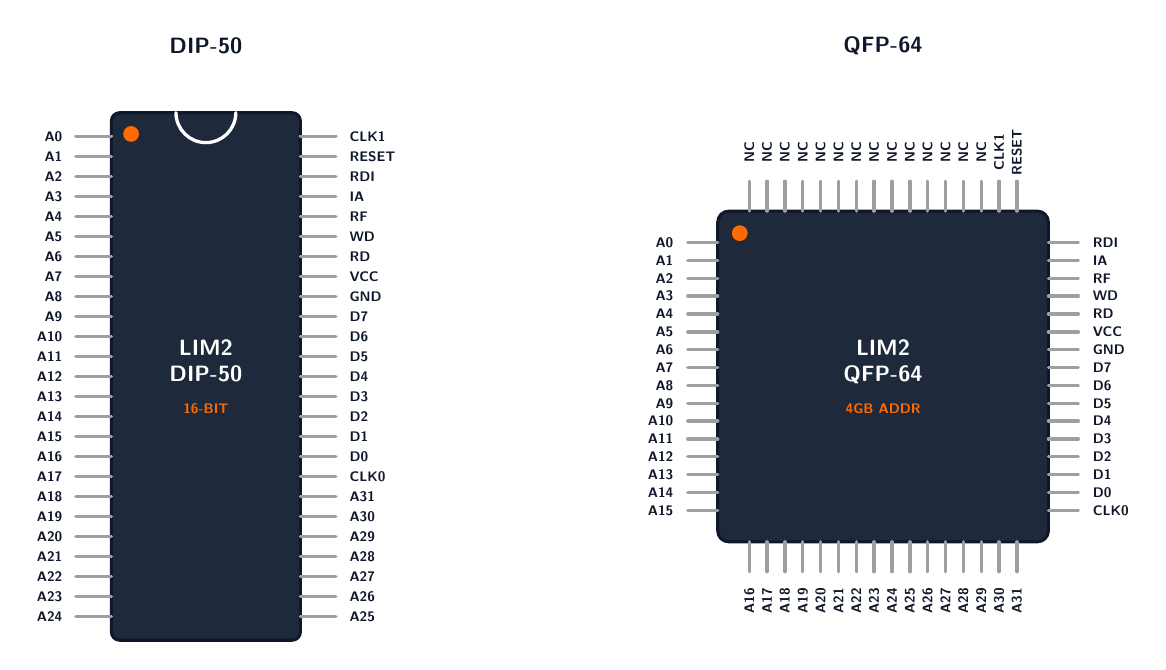
\begin{tikzpicture}[font=\sffamily\scriptsize, line cap=round]
% DIP-50 Package
\node[font=\sffamily\footnotesize\bfseries\color{limslate}] at (-4.1,4.2) {DIP-50};
\draw[rounded corners=3pt, line width=1.1pt, fill=limdark, draw=limslate] (-5.3,-3.35) rectangle (-2.9,3.35);
\draw[line width=1.2pt, color=limwhite!40] (-4.48,3.35) arc (180:360:0.38);
\fill[limorange] (-5.05,3.08) circle (0.10);
\node[align=center, font=\sffamily\footnotesize\bfseries, text=limwhite] at (-4.1,0) {LIM2\\DIP-50\\[2pt]{\tiny\color{limorange}16-BIT}};

\foreach \i/\pinName in {0/A0,1/A1,2/A2,3/A3,4/A4,5/A5,6/A6,7/A7,8/A8,9/A9,10/A10,11/A11,12/A12,13/A13,14/A14,15/A15,16/A16,17/A17,18/A18,19/A19,20/A20,21/A21,22/A22,23/A23,24/A24} {
    \pgfmathsetmacro{\pinY}{3.05 - 0.25417*\i}
    \draw[line width=1.3pt, draw=gray!75!white] (-5.3,\pinY) -- (-5.75,\pinY);
    \node[left, font=\tiny\bfseries\color{limslate}] at (-5.8,\pinY) {\pinName};
}
\foreach \i/\pinName in {0/CLK1,1/RESET,2/RDI,3/IA,4/RF,5/WD,6/RD,7/VCC,8/GND,9/D7,10/D6,11/D5,12/D4,13/D3,14/D2,15/D1,16/D0,17/CLK0,18/A31,19/A30,20/A29,21/A28,22/A27,23/A26,24/A25} {
    \pgfmathsetmacro{\pinY}{3.05 - 0.25417*\i}
    \draw[line width=1.3pt, draw=gray!75!white] (-2.9,\pinY) -- (-2.45,\pinY);
    \node[right, font=\tiny\bfseries\color{limslate}] at (-2.4,\pinY) {\pinName};
}

% QFP-64 Package
\node[font=\sffamily\footnotesize\bfseries\color{limslate}] at (4.5,4.2) {QFP-64};
\draw[rounded corners=4pt, line width=1.1pt, fill=limdark, draw=limslate] (2.4,-2.1) rectangle (6.6,2.1);
\fill[limorange] (2.68,1.82) circle (0.10);
\node[align=center, font=\sffamily\footnotesize\bfseries, text=limwhite] at (4.5,0) {LIM2\\QFP-64\\[2pt]{\tiny\color{limorange}4GB ADDR}};

\foreach \i/\pinName in {0/A0,1/A1,2/A2,3/A3,4/A4,5/A5,6/A6,7/A7,8/A8,9/A9,10/A10,11/A11,12/A12,13/A13,14/A14,15/A15} {
    \pgfmathsetmacro{\pinPos}{1.7 - 0.22667*\i}
    \draw[line width=1.2pt, draw=gray!75!white] (2.4,\pinPos) -- (2.02,\pinPos);
    \node[left, font=\tiny\bfseries\color{limslate}] at (1.96,\pinPos) {\pinName};
}
\foreach \i/\pinName in {0/A16,1/A17,2/A18,3/A19,4/A20,5/A21,6/A22,7/A23,8/A24,9/A25,10/A26,11/A27,12/A28,13/A29,14/A30,15/A31} {
    \pgfmathsetmacro{\pinPos}{-1.7 + 0.22667*\i}
    \pgfmathsetmacro{\pinX}{4.5 + \pinPos}
    \draw[line width=1.2pt, draw=gray!75!white] (\pinX,-2.1) -- (\pinX,-2.48);
    \node[rotate=90, font=\tiny\bfseries\color{limslate}] at (\pinX,-2.85) {\pinName};
}
\foreach \i/\pinName in {0/CLK0,1/D0,2/D1,3/D2,4/D3,5/D4,6/D5,7/D6,8/D7,9/GND,10/VCC,11/RD,12/WD,13/RF,14/IA,15/RDI} {
    \pgfmathsetmacro{\pinPos}{-1.7 + 0.22667*\i}
    \draw[line width=1.2pt, draw=gray!75!white] (6.6,\pinPos) -- (6.98,\pinPos);
    \node[right, font=\tiny\bfseries\color{limslate}] at (7.04,\pinPos) {\pinName};
}
\foreach \i/\pinName in {0/RESET,1/CLK1,2/NC,3/NC,4/NC,5/NC,6/NC,7/NC,8/NC,9/NC,10/NC,11/NC,12/NC,13/NC,14/NC,15/NC} {
    \pgfmathsetmacro{\pinPos}{1.7 - 0.22667*\i}
    \pgfmathsetmacro{\pinX}{4.5 + \pinPos}
    \draw[line width=1.2pt, draw=gray!75!white] (\pinX,2.1) -- (\pinX,2.48);
    \node[rotate=90, font=\tiny\bfseries\color{limslate}] at (\pinX,2.85) {\pinName};
}
\end{tikzpicture}
\caption{Top view of DIP-50 and QFP-64 packages. The orange dot marks Pin 1.}
\end{figure}

\subsection{Pinout Table}
To avoid routing the high-speed clock trace through the middle of the address bus group, the \texttt{A31} and \texttt{CLK0} pins are swapped. Pin assignments 1--50 are identical for DIP-50 and QFP-64; pins 51--64 of the QFP package are not connected (NC).

\begin{table}[htbp]
\centering
\small
\begin{tabularx}{\textwidth}{c l X}
\toprule
\rowcolor{limslate}
\textcolor{white}{\textbf{Pin(s)}} & \textcolor{white}{\textbf{Signal}} & \textcolor{white}{\textbf{Functional Description and Role}} \\
\midrule
\rowcolors{2}{limroweven}{white}
1--32   & \texttt{\textbf{A0--A31}} & 32-bit linear address bus. \\
33      & \texttt{\textbf{CLK0}}   & Primary phase of external clock synchronization. \\
34--41  & \texttt{\textbf{D0--D7}} & 8-bit bidirectional data bus. \\
42      & \texttt{\textbf{GND}}    & System power ground. \\
43      & \texttt{\textbf{VCC}}    & Primary core logic power (+5~V). \\
44      & \texttt{\textbf{RD}}     & Memory / peripheral read strobe (active low). \\
45      & \texttt{\textbf{WD}}     & Memory / peripheral write strobe (active low). \\
46      & \texttt{\textbf{RF}}     & Ready Flag: external device ready acknowledgment. \\
47      & \texttt{\textbf{IA}}     & Interrupt Accepted: interrupt receipt confirmation pulse. \\
48      & \texttt{\textbf{RDI}}    & Raw Direct Interrupt: non-maskable hardware interrupt. \\
49      & \texttt{\textbf{RESET}}  & System master hardware reset input. \\
50      & \texttt{\textbf{CLK1}}   & Secondary phase of external clock synchronization. \\
51--64  & \texttt{\textbf{NC}}     & Reserved unbonded pins (QFP-64 package only). \\
\bottomrule
\end{tabularx}
\caption{Complete Pinout Table for DIP-50 and QFP-64 Packages}
\end{table}

% ==============================================================================
% SECTION 7: INSTRUCTION ENCODING PRINCIPLES
% ==============================================================================
\section{Instruction Encoding Principles}

The LIM2 Instruction Set Architecture (ISA) is based on 32 primary opcodes with extended configuration bytes:

\begin{archcallout}[title={Machine Instruction Encoding Format}]
\begin{itemize}
    \item \textbf{Instruction Length:} Variable — from 1 byte (simple control instructions \texttt{NOP}, \texttt{HALT}) up to 6 bytes (loading immediate 32-bit address/vector constants).
    \item \textbf{First Byte (Opcode):} Contains a 5-bit opcode field (yielding 32 primary instructions) and a 3-bit primary addressing / destination register field.
    \item \textbf{Configuration Byte (Config Byte):} For computational and transfer instructions, the second byte specifies microcode tuning (ALU mode, multiplexer routing, circular shift direction, flag condition inversion).
    \item \textbf{Immediate Operands:} Positioned immediately following the opcode or configuration byte: 1 byte for 8-bit values, 2 bytes for 16-bit words, 4 bytes for addresses and 32-bit vectors.
\end{itemize}
\end{archcallout}


% ==============================================================================
% SECTION 8: LIM2 INSTRUCTION SET ARCHITECTURE
% ==============================================================================
\section{LIM2 Instruction Set Architecture}

The instruction set defines 32 primary opcodes. The summary catalog is provided below, followed by dedicated reference specification pages for each instruction: each entry includes format diagrams, field breakdowns, formal microarchitectural semantics, flag side effects, and practical assembly examples. For instructions with multiple addressing or operand variants, dedicated sub-diagrams and tables are provided.

\subsection{Instruction Quick Catalog}

\small
\noindent
\begin{tabularx}{\textwidth}{@{}c l l >{\raggedright\arraybackslash}X@{}}
\toprule
\rowcolor{limslate}
\textcolor{white}{\textbf{Opcode}} & \textcolor{white}{\textbf{Mnemonic}} & \textcolor{white}{\textbf{Class}} & \textcolor{white}{\textbf{Primary Function}} \\
\midrule
\rowcolors{2}{limroweven}{white}
00000 & \texttt{\textbf{NOP}}  & \textcolor{limmuted}{\textbf{Control}}     & No operation; clears ALU residual latch. \\
00001 & \texttt{\textbf{ADD}}  & \textcolor{limorangeaccent}{\textbf{Arithmetic}} & Addition with automatic carry cascading via ALU residual latch. \\
00010 & \texttt{\textbf{SUB}}  & \textcolor{limorangeaccent}{\textbf{Arithmetic}} & Subtraction with automatic borrow cascading via ALU residual latch. \\
00011 & \texttt{\textbf{MUL}}  & \textcolor{limorangeaccent}{\textbf{Arithmetic}} & Multiplication with upper word capture in ALU residual latch. \\
00100 & \texttt{\textbf{DIV}}  & \textcolor{limorangeaccent}{\textbf{Arithmetic}} & Integer division with remainder capture in internal ALU latch. \\
00101 & \texttt{\textbf{LMR}}  & \textcolor{limdark}{\textbf{Memory}}       & Load into register from memory or input; config 0--3, size 8/16-bit. \\
00110 & \texttt{\textbf{LRM}}  & \textcolor{limdark}{\textbf{Memory}}       & Store from register to memory or output; config 0--2, size 8/16-bit. \\
00111 & \texttt{\textbf{LRR}}  & \textcolor{limdark}{\textbf{Transfer}}     & Direct register-to-register copy via bypass MUX. \\
01000 & \texttt{\textbf{CMP}}  & \textcolor{limorangeaccent}{\textbf{Comparison}} & Hardware operand comparison without modifying register values. \\
01001 & \texttt{\textbf{JMP}}  & \textcolor{limdark}{\textbf{Branch}}       & Unconditional 32-bit jump: direct (5 bytes), indirect, or via PTREG. \\
01010 & \texttt{\textbf{JCR}}  & \textcolor{limdark}{\textbf{Branch}}       & Conditional 32-bit jump on CMP result: $<$, $\le$, $=$, $\ne$, $\ge$, $>$. \\
01011 & \texttt{\textbf{JO / JOB}} & \textcolor{limdark}{\textbf{Branch}}   & Conditional 32-bit jump on overflow or borrow flag (\(\text{OF}=1\) or \(\text{CF}=1\)). \\
01100 & \texttt{\textbf{JZ / JNZ}}  & \textcolor{limdark}{\textbf{Branch}}  & Conditional 32-bit jump on zero flag (bit 2: \(0\) = \texttt{JZ}, \(1\) = \texttt{JNZ}). \\
01101 & \texttt{\textbf{AND}}  & \textcolor{limdark}{\textbf{Logic}}        & Bitwise logical AND (conjunction). \\
01110 & \texttt{\textbf{OR}}   & \textcolor{limdark}{\textbf{Logic}}        & Bitwise logical OR (disjunction). \\
01111 & \texttt{\textbf{NAND}} & \textcolor{limdark}{\textbf{Logic}}        & Bitwise NAND (Sheffer stroke). \\
\bottomrule
\end{tabularx}

\clearpage
\noindent
\begin{tabularx}{\textwidth}{@{}c l l >{\raggedright\arraybackslash}X@{}}
\toprule
\rowcolor{limslate}
\textcolor{white}{\textbf{Opcode}} & \textcolor{white}{\textbf{Mnemonic}} & \textcolor{white}{\textbf{Class}} & \textcolor{white}{\textbf{Primary Function}} \\
\midrule
\rowcolors{2}{limroweven}{white}
10000 & \texttt{\textbf{NOR}}        & \textcolor{limdark}{\textbf{Logic}}        & Bitwise NOR (Peirce arrow). \\
10001 & \texttt{\textbf{NOT}}        & \textcolor{limdark}{\textbf{Logic}}        & Bitwise inversion (ones' complement). \\
10010 & \texttt{\textbf{XOR}}        & \textcolor{limdark}{\textbf{Logic}}        & Bitwise exclusive OR (modulo-2 addition). \\
10011 & \texttt{\textbf{XNOR}}       & \textcolor{limdark}{\textbf{Logic}}        & Bitwise equivalence (inverted XOR). \\
10100 & \texttt{\textbf{INC}}        & \textcolor{limorangeaccent}{\textbf{Arithmetic}} & Hardware operand increment by 1. \\
10101 & \texttt{\textbf{DEC}}        & \textcolor{limorangeaccent}{\textbf{Arithmetic}} & Hardware operand decrement by 1. \\
10110 & \texttt{\textbf{PUSH}}       & \textcolor{limdark}{\textbf{Stack}}        & Push register onto hardware stack space. \\
10111 & \texttt{\textbf{POP}}        & \textcolor{limdark}{\textbf{Stack}}        & Pop top of stack into target register. \\
11000 & \texttt{\textbf{BSL}}        & \textcolor{limorangeaccent}{\textbf{Shifts}}     & Bitwise left shift by 1 with displaced bit capture. \\
11001 & \texttt{\textbf{BSR}}        & \textcolor{limorangeaccent}{\textbf{Shifts}}     & Bitwise right shift by 1 with displaced bit capture. \\
11010 & \texttt{\textbf{MSP}}        & \textcolor{limmuted}{\textbf{System}}      & Special register manipulation (FREG, PTREG, SP, vectors). \\
11011 & \texttt{\textbf{MOD}}        & \textcolor{limorangeaccent}{\textbf{Arithmetic}} & Integer modulo computation (remainder of division). \\
11100 & \texttt{\textbf{INTR / INT}} & \textcolor{limmuted}{\textbf{System}}      & Software interrupt; length 2 bytes, vector IR0--IR15. \\
11101 & \texttt{\textbf{CALL}}       & \textcolor{limdark}{\textbf{Branch}}       & Subroutine call with 32-bit PC pushed to SP stack (modes 0--3). \\
11110 & \texttt{\textbf{RET}}        & \textcolor{limdark}{\textbf{Branch}}       & Subroutine return with 32-bit PC popped from SP stack. \\
11111 & \texttt{\textbf{HALT}}       & \textcolor{limmuted}{\textbf{Control}}     & Hardware processor halt until interrupt or data ready. \\
\bottomrule
\end{tabularx}
\normalsize

% ==============================================================================
% INSTRUCTION DETAILED PAGE TEMPLATE
% ==============================================================================
\newcommand{\instructionpage}[4]{%
\clearpage
\subsection{\texorpdfstring{#2 --- #4}{#2: #3}}

\begin{tcolorbox}[
    enhanced,
    colback=limslate,
    colframe=limslate,
    arc=4pt,
    left=12pt,right=12pt,top=8pt,bottom=8pt,
    drop fuzzy shadow=gray!20
]
    \begin{minipage}[c]{0.35\linewidth}
        {\fontsize{24}{28}\selectfont\bfseries\color{limwhite}\texttt{#2}}
    \end{minipage}\hfill
    \begin{minipage}[c]{0.62\linewidth}
        \raggedleft
        \tcbox[
            enhanced,
            colback=limorange,
            colframe=limorange,
            boxrule=0pt,
            arc=3pt,
            left=6pt,right=6pt,top=2pt,bottom=2pt
        ]{%
            {\footnotesize\bfseries\color{white}OPCODE: \texttt{#1}}%
        }\hspace{0.8em}%
        {\color{limwhite!90}\bfseries\footnotesize [#3]}
    \end{minipage}
\end{tcolorbox}

\vspace{1mm}
\begin{tcolorbox}[
    enhanced,
    colback=limpaper,
    colframe=limborder,
    borderline west={3.5pt}{0pt}{limorange},
    arc=3pt,
    boxrule=0.8pt,
    left=10pt,right=10pt,top=7pt,bottom=7pt
]
    \textbf{\color{limdark}Instruction Purpose:}\par
    \footnotesize #4
\end{tcolorbox}
\vspace{2mm}
}

\newenvironment{instructiondiagram}{%
\par\vspace{2mm}
\noindent\begin{minipage}{\textwidth}
    \centering
    \bytefieldsetup{
        bitformatting={\fontsize{5}{6}\selectfont\color{limmuted}},
        boxformatting={\centering\fontsize{5.2}{6.2}\selectfont}
    }%
}{%
\end{minipage}
\par\vspace{3mm}
}


% ==============================================================================
% 00000: NOP
% ==============================================================================
\instructionpage{00000}{NOP}{Control}{No operation and ALU residual latch reset.}

\subsubsection*{Instruction Format Diagram}
\begin{instructiondiagram}
    \begin{bytefield}[bitwidth=2.4em, endianness=big]{8}
        \bitheader{7,6,5,4,3,2,1,0} \\
        \bitbox{5}{\textbf{OPCODE} = 00000} & \bitbox{3}{\color{limmuted}Ignored}
    \end{bytefield}
\end{instructiondiagram}

\begin{instructiondesc}[title={Detailed Description and Microcode Semantics}]
The \texttt{NOP} (No Operation) instruction performs an idle microcode core cycle:
\begin{itemize}
    \item \textbf{Data Path:} Initiates no read or write bus cycles on the system bus (\texttt{RD=1}, \texttt{WD=1}). Register file multiplexers remain neutral.
    \item \textbf{ALU:} Forcibly flushes internal accumulator buffer latches for remainder and carry cascading, preventing unintended residual effects from preceding mathematical operations.
    \item \textbf{Registers:} Values in general-purpose registers (\texttt{R0--R7}), stack pointer (\texttt{SP}), and address pointer (\texttt{PT}) remain unmodified. The program counter advances normally: \(\texttt{PC} \leftarrow \texttt{PC} + 1\).
\end{itemize}
\end{instructiondesc}

\begin{tcolorbox}[
    enhanced,
    colback=limcard,
    colframe=limborder,
    boxrule=0.6pt,
    arc=3pt,
    left=8pt,right=8pt,top=6pt,bottom=6pt
]
    \footnotesize
    \noindent
    \begin{tabularx}{\textwidth}{@{}l l l X@{}}
        \textbf{Length:} 1 byte &
        \textbf{Operands:} None &
        \textbf{Mode:} User / Supervisor &
        \textbf{Flags affected:} All \texttt{FREG} flags preserved (\texttt{---})
    \end{tabularx}
\end{tcolorbox}

\begin{examplebox}[title={Usage Example (LIM2 Assembly)}]
\begin{limasm}
; 1. Guaranteed flush of ALU residual latch before cascaded calculation
NOP             ; Clear ALU residual register
ADD  \reg0, \reg0, \reg1 ; \reg0 = \reg0 + \reg1 (without previous carry interference)

; 2. Branch target alignment or timing delay (1 clock cycle)
NOP             ; Delay instruction fetch
\end{limasm}
\vspace{1.5mm}
\footnotesize\color{limmuted}
\textbf{Operational Notes:} Invoking \texttt{NOP} before a chain of arithmetic operations guarantees a deterministic baseline state in the ALU. It is also used to generate fixed microsecond timing delays when polling slow external peripherals.
\end{examplebox}

% ------------------------------------------------------------------------------
% 00001: ADD
% ------------------------------------------------------------------------------
\instructionpage{00001}{ADD}{Arithmetic}{Addition with automatic carry cascading via ALU residual latch.}
\subsubsection*{Instruction Format Diagram}
\begin{instructiondiagram}
    \begin{bytefield}[bitwidth=2.4em, endianness=big]{8}
        \bitheader{7,6,5,4,3,2,1,0} \\
        \bitbox{5}{\textbf{OPCODE} = 00001} & \bitbox{3}{Result: (r0-r7)}
    \end{bytefield}
    \begin{bytefield}[bitwidth=2.4em, endianness=big]{8}
        \bitheader{7,6,5,4,3,2,1,0} \\
        \bitbox{3}{Operand 0: (r0-r7)} & \bitbox{3}{Operand 1: (r0-r7)} & \bitbox{2}{Ignored}
    \end{bytefield}
\end{instructiondiagram}

\begin{instructiondesc}[title={Detailed Description and Microcode Semantics}]
The \texttt{ADD} (Addition) instruction computes the sum of two register operands:
\begin{itemize}
    \item \textbf{Data Path:} Computes the sum of numbers from the register pair designated by arguments \texttt{Operand 0} and \texttt{Operand 1}, targeting general-purpose registers \textbf{R0--R7}.
    \item \textbf{ALU Cascading:} If preceding arithmetic operations produced a carry stored in the ALU residual latch, it is automatically incorporated into the summation.
    \item \textbf{Registers:} The computed sum is stored in the destination register specified by \texttt{Result} (\texttt{R0--R7}).
\end{itemize}
\end{instructiondesc}

\begin{tcolorbox}[
    enhanced,
    colback=limcard,
    colframe=limborder,
    boxrule=0.6pt,
    arc=3pt,
    left=8pt,right=8pt,top=6pt,bottom=6pt
]
    \footnotesize
    \noindent
    \begin{tabularx}{\textwidth}{@{}l l l X@{}}
        \textbf{Length:} 2 bytes &
        \textbf{Operands:} 3 &
        \textbf{Mode:} User / Supervisor &
        \textbf{Flags affected:} In case of arithmetic carry, bit \texttt{CF} is asserted to log. 1.
    \end{tabularx}
\end{tcolorbox}

\begin{examplebox}[title={Usage Example (LIM2 Assembly)}]
\begin{limasm}
ADD  \reg0, \reg1, \reg2     ; \reg0 = \reg1 + \reg2 
\end{limasm}
\vspace{1.5mm}
\footnotesize\color{limmuted}
\textbf{Operational Notes:} The \texttt{ADD} instruction adds values from two user registers. In the event of an arithmetic carry, the \texttt{CF} flag in \texttt{FREG} is asserted to logical 1.
\end{examplebox}

% ------------------------------------------------------------------------------
% 00010: SUB
% ------------------------------------------------------------------------------
\instructionpage{00010}{SUB}{Arithmetic}{Subtraction with automatic borrow cascading via ALU residual latch.}
\subsubsection*{Instruction Format Diagram}
\begin{instructiondiagram}
    \begin{bytefield}[bitwidth=2.4em, endianness=big]{8}
        \bitheader{7,6,5,4,3,2,1,0} \\
        \bitbox{5}{\textbf{OPCODE} = 00010} & \bitbox{3}{Result: \texttt{R0-R7}}
    \end{bytefield}
    \begin{bytefield}[bitwidth=2.4em, endianness=big]{8}
        \bitheader{7,6,5,4,3,2,1,0} \\
        \bitbox{3}{Operand 0: \texttt{R0-R7}} & \bitbox{3}{Operand 1: \texttt{R0-R7}} & \bitbox{2}{Ignored}
    \end{bytefield}
\end{instructiondiagram}

\begin{instructiondesc}[title={Detailed Description and Microcode Semantics}]
The \texttt{SUB} (Subtraction) instruction computes the arithmetic difference between two registers:
\begin{itemize}
    \item \textbf{Data Path:} Computes the difference between register operands designated by \texttt{Operand 0} and \texttt{Operand 1}, corresponding to general-purpose registers \textbf{R0--R7}.
    \item \textbf{ALU Borrow:} If preceding operations generated a borrow condition latched in the ALU residual buffer, it is automatically accounted for in the subtraction.
    \item \textbf{Registers:} The difference is stored in the destination register specified by \texttt{Result} (\texttt{R0--R7}).
\end{itemize}
\end{instructiondesc}

\begin{tcolorbox}[
    enhanced,
    colback=limcard,
    colframe=limborder,
    boxrule=0.6pt,
    arc=3pt,
    left=8pt,right=8pt,top=6pt,bottom=6pt
]
    \footnotesize
    \noindent
    \begin{tabularx}{\textwidth}{@{}l l l X@{}}
        \textbf{Length:} 2 bytes &
        \textbf{Operands:} 3 &
        \textbf{Mode:} User / Supervisor &
        \textbf{Flags affected:} In case of borrow, bit \texttt{CF} is asserted to log. 1.
    \end{tabularx}
\end{tcolorbox}

\begin{examplebox}[title={Usage Example (LIM2 Assembly)}]
\begin{limasm}
SUB  \reg0, \reg1, \reg2     ; \reg0 = \reg1 - \reg2 
\end{limasm}
\vspace{1.5mm}
\footnotesize\color{limmuted}
\textbf{Operational Notes:} The \texttt{SUB} instruction subtracts the second user register from the first. When a borrow occurs, the \texttt{CF} flag in \texttt{FREG} is asserted to logical 1.
\end{examplebox}

% ------------------------------------------------------------------------------
% 00011: MUL
% ------------------------------------------------------------------------------
\instructionpage{00011}{MUL}{Arithmetic}{Multiplication with upper word capture in ALU residual latch.}
\subsubsection*{Instruction Format Diagram}
\begin{instructiondiagram}
    \begin{bytefield}[bitwidth=2.4em, endianness=big]{8}
        \bitheader{7,6,5,4,3,2,1,0} \\
        \bitbox{5}{\textbf{OPCODE} = 00011} & \bitbox{3}{Result: \texttt{R0-R7}}
    \end{bytefield}
    \begin{bytefield}[bitwidth=2.4em, endianness=big]{8}
        \bitheader{7,6,5,4,3,2,1,0} \\
        \bitbox{3}{Operand 0: \texttt{R0-R7}} & \bitbox{3}{Operand 1: \texttt{R0-R7}} & \bitbox{2}{Ignored}
    \end{bytefield}
\end{instructiondiagram}

\begin{instructiondesc}[title={Detailed Description and Microcode Semantics}]
The \texttt{MUL} (Multiply) instruction computes the product of two register operands:
\begin{itemize}
    \item \textbf{Data Path:} Computes the product of operands from the register pair designated by \texttt{Operand 0} and \texttt{Operand 1}, pointing to user registers \textbf{R0--R7}.
    \item \textbf{Residual Accumulator:} The lower 16 bits of the 32-bit product are placed in the \texttt{Result} register, while the upper 16 bits are captured into the internal post-arithmetic ALU accumulator latch.
    \item \textbf{Registers:} The low word of the result is stored into \texttt{Result} (\texttt{R0--R7}).
\end{itemize}
\end{instructiondesc}

\begin{tcolorbox}[
    enhanced,
    colback=limcard,
    colframe=limborder,
    boxrule=0.6pt,
    arc=3pt,
    left=8pt,right=8pt,top=6pt,bottom=6pt
]
    \footnotesize
    \noindent
    \begin{tabularx}{\textwidth}{@{}l l l X@{}}
        \textbf{Length:} 2 bytes &
        \textbf{Operands:} 3 &
        \textbf{Mode:} User / Supervisor &
        \textbf{Flags affected:} On arithmetic overflow, bit \texttt{OF} is asserted to log. 1.
    \end{tabularx}
\end{tcolorbox}

\begin{examplebox}[title={Usage Example (LIM2 Assembly)}]
\begin{limasm}
MUL  \reg0, \reg1, \reg2     ; \reg0 = \reg1 * \reg2 
\end{limasm}
\vspace{1.5mm}
\footnotesize\color{limmuted}
\textbf{Operational Notes:} The \texttt{MUL} instruction multiplies two values from user registers. If an overflow occurs, flags \texttt{CF} and \texttt{OF} are asserted to logical 1, and the post-arithmetic accumulator captures the upper 16 bits of the product.
\end{examplebox}
The multiplication operation in the \textbf{LIM2} ALU is single-cycle in silicon, though the complete instruction takes multiple clock phases due to the microcoded core sequencing.

% ------------------------------------------------------------------------------
% 00100: DIV
% ------------------------------------------------------------------------------
\instructionpage{00100}{DIV}{Arithmetic}{Division with remainder capture in internal ALU latch.}
\subsubsection*{Instruction Format Diagram}
\begin{instructiondiagram}
    \begin{bytefield}[bitwidth=2.4em, endianness=big]{8}
        \bitheader{7,6,5,4,3,2,1,0} \\
        \bitbox{5}{\textbf{OPCODE} = 00100} & \bitbox{3}{Result: \texttt{R0-R7}}
    \end{bytefield}
    \begin{bytefield}[bitwidth=2.4em, endianness=big]{8}
        \bitheader{7,6,5,4,3,2,1,0} \\
        \bitbox{3}{Operand 0: \texttt{R0-R7}} & \bitbox{3}{Operand 1: \texttt{R0-R7}} & \bitbox{2}{Ignored}
    \end{bytefield}
\end{instructiondiagram}

\begin{instructiondesc}[title={Detailed Description and Microcode Semantics}]
The \texttt{DIV} (Divide) instruction calculates the integer quotient of two register values:
\begin{itemize}
    \item \textbf{Data Path:} Computes the integer quotient of the pair of registers designated by \texttt{Operand 0} and \texttt{Operand 1}, targeting user registers \textbf{R0--R7}.
    \item \textbf{Corner Cases:} The minimum result in integer division is 0, including cases where \( 1 > \frac{A}{B} > 0\). In such cases, \texttt{ZF} is asserted to logical 1 and the resulting quotient is 0. Division by zero triggers the \texttt{EM} math fault and vectors to ISR 1.
\end{itemize}
\end{instructiondesc}

\begin{tcolorbox}[
    enhanced,
    colback=limcard,
    colframe=limborder,
    boxrule=0.6pt,
    arc=3pt,
    left=8pt,right=8pt,top=6pt,bottom=6pt
]
    \footnotesize
    \noindent
    \begin{tabularx}{\textwidth}{@{}l l l X@{}}
        \textbf{Length:} 2 bytes &
        \textbf{Operands:} 3 &
        \textbf{Mode:} User / Supervisor &
        \textbf{Flags affected:} On arithmetic overflow, bit \texttt{OF} is asserted to log. 1.
    \end{tabularx}
\end{tcolorbox}

\begin{examplebox}[title={Usage Example (LIM2 Assembly)}]
\begin{limasm}
DIV  \reg0, \reg1, \reg2     ; \reg0 = \reg1 // \reg2 
\end{limasm}
\vspace{1.5mm}
\footnotesize\color{limmuted}
\textbf{Operational Notes:} The \texttt{DIV} instruction performs integer division between user registers. If \( 1 > \frac{A}{B} > 0\), the result is set to 0 and the \texttt{ZF} flag is asserted to logical 1.
\end{examplebox}


% ------------------------------------------------------------------------------
% 00101: LMR
% ------------------------------------------------------------------------------
\instructionpage{00101}{LMR}{Memory}{Load into register from memory or input; source config 0--3, size 8/16-bit.}
\subsubsection*{Instruction Format Diagram}
\begin{instructiondiagram}
    \begin{bytefield}[bitwidth=2.4em, endianness=big]{8}
        \bitheader{7,6,5,4,3,2,1,0} \\
        \bitbox{5}{\textbf{OPCODE} = 00101} & \bitbox{1}{\textbf{DS} = 0/1} & \bitbox{2}{Source 0-3}
    \end{bytefield}
\end{instructiondiagram}

\begin{instructiondesc}[title={Detailed Description and Microcode Semantics}]
The \texttt{LMR} (Load from Memory to Register) instruction loads data from memory into a general-purpose register:
\begin{itemize}
    \item \textbf{Data Path:} Loads a byte or word from memory into the selected destination register.
    \item \textbf{Modes and Configuration:} The DS (Data Size) bit specifies the operand width: \\
    \( DS = 0 \rightarrow 1\text{ byte} \) \\
    \( DS = 1 \rightarrow 2\text{ bytes (word)} \) \\
    This configuration does not modify the structure of subsequent arguments or addressing options.
    \item \textbf{Data Width Mnemonics:} To select operand width in LIM2 assembly, the \texttt{.b / .w} suffix is used.
\end{itemize}
\end{instructiondesc}

\subsubsection*{Immediate Data Load Mode (Source = 0b00)}
\begin{instructiondiagram}
    \begin{bytefield}[bitwidth=2em, endianness=big]{8}
        \bitheader{7,6,5,4,3,2,1,0} \\
        \bitbox{5}{\textbf{OPCODE} = 00101} & \bitbox{1}{\textbf{DS} = 0/1} & \bitbox{2}{Source = 0b00}
    \end{bytefield}
    \begin{bytefield}[bitwidth=2em, endianness=big]{8}
        \bitheader{7,6,5,4,3,2,1,0} \\
        \bitbox{3}{Target: (R0-R7)} & \bitbox{5}{Ignored}
    \end{bytefield}
    \begin{bytefield}[bitwidth=0.6em, endianness=big]{8}
        \bitheader{7,6,5,4,3,2,1,0} \\
        \bitbox{8}{\textbf{BYTE lo}} 
    \end{bytefield}
    \begin{bytefield}[bitwidth=0.6em, endianness=big]{8}
        \bitheader{7,6,5,4,3,2,1,0} \\
        \bitbox{8}{\textbf{BYTE hi}} 
    \end{bytefield}
\end{instructiondiagram}

\begin{instructiondesc}[title={Immediate Data Load Mode}]
The \texttt{LMR} instruction when \textbf{SOURCE = 0b00}:
\begin{itemize}
    \item \textbf{Data Path:} When \textbf{Source = 0b00}, the instruction loads an immediate byte/word directly into the target register: data follows immediately after the instruction opcode in memory, following Little-Endian order (lower byte at lower address).
    \item \textbf{Modes and Configuration:} The DS (Data Size) bit specifies the size: \\
    \( DS = 0 \rightarrow 1\text{ byte} \) \\
    \( DS = 1 \rightarrow 2\text{ bytes (word)} \)
    \item \textbf{Data Width Mnemonics:} Selected via \texttt{.b} or \texttt{.w} suffix in assembly.
\end{itemize}
\end{instructiondesc}

\subsubsection*{Direct Address Load Mode (Source = 0b01)}
\begin{instructiondiagram}
    \begin{bytefield}[bitwidth=1.9em, endianness=big]{8}
        \bitheader{7,6,5,4,3,2,1,0} \\
        \bitbox{5}{\textbf{OPCODE} = 00101} & \bitbox{1}{\textbf{DS} = 0/1} & \bitbox{2}{Source = 0b01}
    \end{bytefield}
    \begin{bytefield}[bitwidth=1.9em, endianness=big]{8}
        \bitheader{7,6,5,4,3,2,1,0} \\
        \bitbox{3}{Target: (R0-R7)} & \bitbox{5}{Ignored}
    \end{bytefield}
    \begin{bytefield}[bitwidth=0.35em, endianness=big]{8}
        \bitheader{7,6,5,4,3,2,1,0} \\
        \bitbox{8}{\textbf{ADDR lo}} 
    \end{bytefield}
    \begin{bytefield}[bitwidth=0.35em, endianness=big]{8}
        \bitheader{7,6,5,4,3,2,1,0} \\
        \bitbox{8}{\textbf{ADDR lo-hi}} 
    \end{bytefield}
    \begin{bytefield}[bitwidth=0.35em, endianness=big]{8}
        \bitheader{7,6,5,4,3,2,1,0} \\
        \bitbox{8}{\textbf{ADDR hi-lo}} 
    \end{bytefield}
    \begin{bytefield}[bitwidth=0.35em, endianness=big]{8}
        \bitheader{7,6,5,4,3,2,1,0} \\
        \bitbox{8}{\textbf{ADDR hi}} 
    \end{bytefield}
\end{instructiondiagram}

\begin{instructiondesc}[title={Direct Address Load Mode}]
The \texttt{LMR} instruction when \textbf{SOURCE = 0b01}:
\begin{itemize}
    \item \textbf{Data Path:} When \textbf{Source = 0b01}, the instruction loads a byte/word from memory into the selected register using an immediate 32-bit physical address (4 bytes) following the instruction, adhering to Little-Endian order.
    \item \textbf{Modes and Configuration:} The DS (Data Size) bit specifies the operand size: \\
    \( DS = 0 \rightarrow 1\text{ byte} \) \\
    \( DS = 1 \rightarrow 2\text{ bytes (word)} \)
    \item This instruction variant occupies 6 bytes of memory (2 opcode/config bytes + 4 address bytes).
    \item \textbf{Data Width Mnemonics:} Selected via \texttt{.b} or \texttt{.w} suffix in assembly.
\end{itemize}
\end{instructiondesc}

\subsubsection*{Pointer Register Indirect Load Mode (Source = 0b10)}
\begin{instructiondiagram}
    \begin{bytefield}[bitwidth=2.4em, endianness=big]{8}
        \bitheader{7,6,5,4,3,2,1,0} \\
        \bitbox{5}{\textbf{OPCODE} = 00101} & \bitbox{1}{\textbf{DS} = 0/1} & \bitbox{2}{Source = 0b10}
    \end{bytefield}
    \begin{bytefield}[bitwidth=2em, endianness=big]{8}
        \bitheader{7,6,5,4,3,2,1,0} \\
        \bitbox{3}{Target: (R0-R7)} & \bitbox{5}{Ignored}
    \end{bytefield}
\end{instructiondiagram}

\begin{instructiondesc}[title={Pointer Register Indirect Load Mode}]
The \texttt{LMR} instruction when \textbf{SOURCE = 0b10}:
\begin{itemize}
    \item \textbf{Data Path:} When \textbf{Source = 0b10}, the instruction loads a byte/word from memory into the destination register via the address contained in \texttt{Pointer Register (PTREG)}. This provides high efficiency for streaming and sequential block transfers.
    \item \textbf{Modes and Auto-Increment:} The DS bit defines data width: \\
    \( DS = 0 \rightarrow 1\text{ byte} \) \\
    \( DS = 1 \rightarrow 2\text{ bytes (word)} \) \\
    When auto-increment is enabled (\texttt{AIP=1} in \texttt{FREG}), accessing memory through \texttt{PTREG} automatically increments its value by the transfer size (+1 or +2), dramatically accelerating data stream processing.
    \item This instruction variant occupies 2 bytes of memory.
    \item \textbf{Data Width Mnemonics:} Selected via \texttt{.b} or \texttt{.w} suffix in assembly.
\end{itemize}
\end{instructiondesc}

\subsubsection*{Register Pair Indirect Load Mode (Source = 0b11)}
\begin{instructiondiagram}
    \begin{bytefield}[bitwidth=2.4em, endianness=big]{8}
        \bitheader{7,6,5,4,3,2,1,0} \\
        \bitbox{5}{\textbf{OPCODE} = 00101} & \bitbox{1}{\textbf{DS} = 0/1} & \bitbox{2}{Source = 0b11}
    \end{bytefield}
    \begin{bytefield}[bitwidth=2.4em, endianness=big]{8}
        \bitheader{7,6,5,4,3,2,1,0} \\
        \bitbox{3}{Source/Target 0: (R0-R7)} & \bitbox{3}{Source 0: (R0-R7)} & \bitbox{2}{Ignored}
    \end{bytefield}
\end{instructiondiagram}

\begin{instructiondesc}[title={Register Pair Indirect Load Mode}]
The \texttt{LMR} instruction when \textbf{SOURCE = 0b11}:
\begin{itemize}
    \item \textbf{Data Path:} When \textbf{Source = 0b11}, the instruction forms a 32-bit effective address from a pair of user registers according to: \( (Rx \ll 16) \mid Ry \). The loaded data is stored into the register that held the upper address bits: \( Rx = [(Rx \ll 16) \mid Ry] \).
    \item \textbf{Modes and Configuration:} The DS bit specifies the operand width: \\
    \( DS = 0 \rightarrow 1\text{ byte} \) \\
    \( DS = 1 \rightarrow 2\text{ bytes (word)} \) \\
    Because the register holding the upper address is overwritten by the loaded data, duplicated copies should be maintained if the pointer is reused.
    \item This instruction variant occupies 2 bytes of memory.
    \item \textbf{Data Width Mnemonics:} Selected via \texttt{.b} or \texttt{.w} suffix in assembly.
\end{itemize}
\end{instructiondesc}

\begin{tcolorbox}[
    enhanced,
    colback=limcard,
    colframe=limborder,
    boxrule=0.6pt,
    arc=3pt,
    left=8pt,right=8pt,top=6pt,bottom=6pt
]
    \footnotesize
    \noindent
    \begin{tabularx}{\textwidth}{@{}l l l X@{}}
        \textbf{Length:} 2--6 bytes &
        \textbf{Operands:} 2--3 &
        \textbf{Mode:} User / Supervisor &
        \textbf{Flags affected:} On arithmetic overflow, bit \texttt{OF} is asserted to log. 1.
    \end{tabularx}
\end{tcolorbox}

\begin{examplebox}[title={Usage Example (LIM2 Assembly)}]
\begin{limasm}
;============================
; 1. Immediate data load into register
LMR.b \reg0, 0xFFFF         ; \reg0 = 0x00FF (byte mode selected)
;============================
; 2. Data load from direct 32-bit address
LMR.w \reg0, [0xF000]       ; \reg0 = Memory[0xF000 .. 0xF001]
;============================
; 3. Data load via pointer register PTREG
LMR \reg0, [\regPTREG]      ; \reg0 = Memory[$PTREG] (auto-increments PTREG)
;============================
; 4. Data load via compound 32-bit register pair pointer
LMR \reg0, [\reg0:\reg1]    ; \reg0 = Memory[(\reg0 << 16 | \reg1)] (word)
\end{limasm}
\vspace{1.5mm}
\footnotesize\color{limmuted}
\textbf{Operational Notes:} The \texttt{LMR} instruction loads an 8-bit or 16-bit value from memory or an I/O device into a general-purpose register.
\end{examplebox}

\subsection{Assembler Convention:}

\begin{securitycallout}[title={Default Data Width Assumption}]
\begin{itemize}
    \item When no explicit operand width suffix is specified in memory load/store instructions, the assembler defaults to word mode (word / 16-bit / 2 bytes), as this provides maximum performance and code clarity.
\end{itemize}
\end{securitycallout}

% ------------------------------------------------------------------------------
% 00110: LRM
% ------------------------------------------------------------------------------
\instructionpage{00110}{LRM}{Memory}{Store from register to memory or output; config 0--2, size 8/16-bit.}
\subsubsection*{Instruction Format Diagram}
\begin{instructiondiagram}
    \begin{bytefield}[bitwidth=2.4em, endianness=big]{8}
        \bitheader{7,6,5,4,3,2,1,0} \\
        \bitbox{5}{\textbf{OPCODE} = 00110} & \bitbox{1}{\textbf{DS} = 0/1} & \bitbox{2}{Source 0-2}
    \end{bytefield}
\end{instructiondiagram}

\begin{instructiondesc}[title={Detailed Description and Microcode Semantics}]
The \texttt{LRM} (Load to Memory from Register / Store Register to Memory) instruction stores data from registers into memory:
\begin{itemize}
    \item \textbf{Data Path:} Stores a byte/word from a selected user register (or immediate constant) into system memory.
    \item \textbf{Modes and Configuration:} The DS (Data Size) bit specifies the operand width: \\
    \( DS = 0 \rightarrow 1\text{ byte} \) \\
    \( DS = 1 \rightarrow 2\text{ bytes (word)} \) \\
    This configuration does not modify the addressing parameters.
    \item \textbf{Data Width Mnemonics:} Selected via \texttt{.b} or \texttt{.w} suffix in assembly.
\end{itemize}
\end{instructiondesc}

\subsubsection*{Immediate Data Store to Memory (Source = 0b00)}
\begin{instructiondiagram}
    \begin{bytefield}[bitwidth=2em, endianness=big]{8}
        \bitheader{7,6,5,4,3,2,1,0} \\
        \bitbox{5}{\textbf{OPCODE} = 00110} & \bitbox{1}{\textbf{DS} = 0/1} & \bitbox{2}{Source = 0b00}
    \end{bytefield}
    \begin{bytefield}[bitwidth=2em, endianness=big]{8}
        \bitheader{7,6,5,4,3,2,1,0} \\
        \bitbox{3}{Source: (R0-R7)} & \bitbox{5}{Ignored}
    \end{bytefield}
    \begin{bytefield}[bitwidth=0.6em, endianness=big]{8}
        \bitheader{7,6,5,4,3,2,1,0} \\
        \bitbox{8}{\textbf{BYTE lo}} 
    \end{bytefield}
    \begin{bytefield}[bitwidth=0.6em, endianness=big]{8}
        \bitheader{7,6,5,4,3,2,1,0} \\
        \bitbox{8}{\textbf{BYTE hi}} 
    \end{bytefield}
\end{instructiondiagram}

\begin{instructiondesc}[title={Immediate Data Store Mode}]
The \texttt{LRM} instruction when \textbf{SOURCE = 0b00}:
\begin{itemize}
    \item \textbf{Data Path:} When \textbf{Source = 0b00}, the instruction writes immediate byte/word data into memory at the address currently pointed to by \texttt{Pointer Register (PTREG)}: the immediate value follows the instruction in memory (Little-Endian order).
    \item \textbf{Modes and Auto-Increment:} The DS bit defines data width: \\
    \( DS = 0 \rightarrow 1\text{ byte} \) \\
    \( DS = 1 \rightarrow 2\text{ bytes (word)} \) \\
    Writing data automatically advances \texttt{Pointer Register (PTREG)} by the written size (1 or 2 bytes).
    \item This instruction variant occupies 4 bytes of memory (for $DS=1$).
    \item \textbf{Data Width Mnemonics:} Selected via \texttt{.b} or \texttt{.w} suffix in assembly.
\end{itemize}
\end{instructiondesc}

\subsubsection*{Direct Address Store Mode (Source = 0b01)}
\begin{instructiondiagram}
    \begin{bytefield}[bitwidth=1.9em, endianness=big]{8}
        \bitheader{7,6,5,4,3,2,1,0} \\
        \bitbox{5}{\textbf{OPCODE} = 00110} & \bitbox{1}{\textbf{DS} = 0/1} & \bitbox{2}{Source = 0b01}
    \end{bytefield}
    \begin{bytefield}[bitwidth=1.9em, endianness=big]{8}
        \bitheader{7,6,5,4,3,2,1,0} \\
        \bitbox{3}{Source: (R0-R7)} & \bitbox{5}{Ignored}
    \end{bytefield}
    \begin{bytefield}[bitwidth=0.35em, endianness=big]{8}
        \bitheader{7,6,5,4,3,2,1,0} \\
        \bitbox{8}{\textbf{ADDR lo}} 
    \end{bytefield}
    \begin{bytefield}[bitwidth=0.35em, endianness=big]{8}
        \bitheader{7,6,5,4,3,2,1,0} \\
        \bitbox{8}{\textbf{ADDR lo-hi}} 
    \end{bytefield}
    \begin{bytefield}[bitwidth=0.35em, endianness=big]{8}
        \bitheader{7,6,5,4,3,2,1,0} \\
        \bitbox{8}{\textbf{ADDR hi-lo}} 
    \end{bytefield}
    \begin{bytefield}[bitwidth=0.35em, endianness=big]{8}
        \bitheader{7,6,5,4,3,2,1,0} \\
        \bitbox{8}{\textbf{ADDR hi}} 
    \end{bytefield}
\end{instructiondiagram}

\begin{instructiondesc}[title={Direct Address Store Mode}]
The \texttt{LRM} instruction when \textbf{SOURCE = 0b01}:
\begin{itemize}
    \item \textbf{Data Path:} When \textbf{Source = 0b01}, the instruction stores a byte/word from the selected user register into memory at the absolute 32-bit physical address (4 bytes) immediately following the instruction in Little-Endian format.
    \item \textbf{Modes and Configuration:} The DS bit defines data width: \\
    \( DS = 0 \rightarrow 1\text{ byte} \) \\
    \( DS = 1 \rightarrow 2\text{ bytes (word)} \)
    \item This instruction variant occupies 6 bytes of memory.
    \item \textbf{Data Width Mnemonics:} Selected via \texttt{.b} or \texttt{.w} suffix in assembly.
\end{itemize}
\end{instructiondesc}

\subsubsection*{Pointer Register Indirect Store Mode (Source = 0b10)}
\begin{instructiondiagram}
    \begin{bytefield}[bitwidth=2.4em, endianness=big]{8}
        \bitheader{7,6,5,4,3,2,1,0} \\
        \bitbox{5}{\textbf{OPCODE} = 00110} & \bitbox{1}{\textbf{DS} = 0/1} & \bitbox{2}{Source = 0b10}
    \end{bytefield}
    \begin{bytefield}[bitwidth=2em, endianness=big]{8}
        \bitheader{7,6,5,4,3,2,1,0} \\
        \bitbox{3}{Source: (R0-R7)} & \bitbox{5}{Ignored}
    \end{bytefield}
\end{instructiondiagram}

\begin{instructiondesc}[title={Pointer Register Indirect Store Mode}]
The \texttt{LRM} instruction when \textbf{SOURCE = 0b10}:
\begin{itemize}
    \item \textbf{Data Path:} When \textbf{Source = 0b10}, the instruction stores a byte/word from the chosen register into memory at the address specified by \texttt{Pointer Register (PTREG)}.
    \item \textbf{Modes and Auto-Increment:} The DS bit defines data width: \\
    \( DS = 0 \rightarrow 1\text{ byte} \) \\
    \( DS = 1 \rightarrow 2\text{ bytes (word)} \) \\
    When auto-increment is active, storing data automatically increases \texttt{PTREG} by the transferred width (+1 or +2 bytes), enabling fast sequential writes.
    \item This instruction variant occupies 2 bytes of memory.
    \item \textbf{Data Width Mnemonics:} Selected via \texttt{.b} or \texttt{.w} suffix in assembly.
\end{itemize}
\end{instructiondesc}

\begin{instructiondesc}[title={Architectural Note: Absence of Compound Register-Pair Store Mode (0b11)}]
Unlike \texttt{LMR}, the \texttt{LRM} instruction \textbf{does not support} compound address mode via register pairs (\textbf{Source = 0b11}). The bit combination \texttt{11} is reserved. For indirect addressing, the target address is loaded into \texttt{PTREG}.
\end{instructiondesc}

\begin{tcolorbox}[
    enhanced,
    colback=limcard,
    colframe=limborder,
    boxrule=0.6pt,
    arc=3pt,
    left=8pt,right=8pt,top=6pt,bottom=6pt
]
    \footnotesize
    \noindent
    \begin{tabularx}{\textwidth}{@{}l l l X@{}}
        \textbf{Length:} 2--6 bytes &
        \textbf{Operands:} 2 &
        \textbf{Mode:} User / Supervisor &
        \textbf{Flags affected:} Flags preserved (no effect on \texttt{FREG}).
    \end{tabularx}
\end{tcolorbox}

\begin{examplebox}[title={Usage Example (LIM2 Assembly)}]
\begin{limasm}
;============================
; 1. Store immediate data to memory via PTREG
LRM.b  [\regPTREG], 0xFFFF  ; Memory[$PTREG] = 0x00FF (increments PTREG by 1)
;============================
; 2. Store register value to direct 32-bit address
LRM.w  [0xF000], \reg0      ; Memory[0xF000] = $0
;============================
; 3. Store register value via pointer PTREG
LRM  [\regPTREG], \reg0     ; Memory[$PTREG] = $0 (increments PTREG by 2)
\end{limasm}
\vspace{1.5mm}
\footnotesize\color{limmuted}
\textbf{Operational Notes:} The \texttt{LRM} instruction stores data from a user register or immediate constant into memory. Addressing via \texttt{PTREG} automatically advances the pointer by the written data width.
\end{examplebox}

\subsection{Assembler Convention:}

\begin{securitycallout}[title={Default Data Width Assumption}]
\begin{itemize}
    \item When no explicit operand width suffix is specified in memory store instructions, the assembler defaults to word mode (word / 16-bit / 2 bytes).
\end{itemize}
\end{securitycallout}

% ------------------------------------------------------------------------------
% 00111: LRR
% ------------------------------------------------------------------------------
\instructionpage{00111}{LRR}{Transfer}{Direct register-to-register copy via bypass MUX.}
\subsubsection*{Instruction Format Diagram}
\begin{instructiondiagram}
    \begin{bytefield}[bitwidth=2.4em, endianness=big]{8}
        \bitheader{7,6,5,4,3,2,1,0} \\
        \bitbox{5}{\textbf{OPCODE} = 00111} & \bitbox{3}{Target: (R0-R7)}
    \end{bytefield}
    \begin{bytefield}[bitwidth=2.4em, endianness=big]{8}
        \bitheader{7,6,5,4,3,2,1,0} \\
        \bitbox{3}{Source: (R0-R7)} & \bitbox{5}{Ignored}
    \end{bytefield}
\end{instructiondiagram}

\begin{instructiondesc}[title={Detailed Description and Microcode Semantics}]
The \texttt{LRR} (Load Register to Register) instruction copies data between registers:
\begin{itemize}
    \item \textbf{Data Path:} Direct transfer of 16-bit word data from one user register to another via the internal bypass multiplexer. Register-to-register copying is always strictly 16-bit (word).
\end{itemize}
\end{instructiondesc}

\begin{tcolorbox}[
    enhanced,
    colback=limcard,
    colframe=limborder,
    boxrule=0.6pt,
    arc=3pt,
    left=8pt,right=8pt,top=6pt,bottom=6pt
]
    \footnotesize
    \noindent
    \begin{tabularx}{\textwidth}{@{}l l l X@{}}
        \textbf{Length:} 2 bytes &
        \textbf{Operands:} 2 &
        \textbf{Mode:} User / Supervisor &
        \textbf{Flags affected:} Flags preserved (no effect on \texttt{FREG}).
    \end{tabularx}
\end{tcolorbox}

\begin{examplebox}[title={Usage Example (LIM2 Assembly)}]
\begin{limasm}
LRR \reg0, \reg1  ; \reg0 = \reg1 (Register Copy)
\end{limasm}
\vspace{1.5mm}
\footnotesize\color{limmuted}
\textbf{Operational Notes:} The \texttt{LRR} instruction copies data from \texttt{Source (\reg0--\reg7)} into \texttt{Target (\reg0--\reg7)}.
\end{examplebox}


% ------------------------------------------------------------------------------
% 01000: CMP
% ------------------------------------------------------------------------------
\instructionpage{01000}{CMP}{Comparison}{Hardware operand comparison without modifying register values.}
\subsubsection*{Instruction Format Diagram}
\begin{instructiondiagram}
    \begin{bytefield}[bitwidth=2.4em, endianness=big]{8}
        \bitheader{7,6,5,4,3,2,1,0} \\
        \bitbox{5}{\textbf{OPCODE} = 01000} & \bitbox{3}{Operand 0: (\reg0-\reg7)}
    \end{bytefield}
    \begin{bytefield}[bitwidth=2.4em, endianness=big]{8}
        \bitheader{7,6,5,4,3,2,1,0} \\
        \bitbox{3}{Operand 1: (\reg0-\reg7)} & \bitbox{5}{Ignored} 
    \end{bytefield}
\end{instructiondiagram}

\begin{instructiondesc}[title={Detailed Description and Microcode Semantics}]
The \texttt{CMP} (Compare) instruction performs an integer comparison between two register operands without altering their values:
\begin{itemize}
    \item \textbf{Data Path:} Compares numbers in the designated registers and records the comparison outcome in bits 4--5 of \texttt{FREG} (\texttt{CMP} bits). Comparison is single-cycle in the ALU.
    \item \textbf{Result Encoding:} The \texttt{CMP} bit field states are defined as follows: \\
    \( CMP = 0b00 \rightarrow \text{No operation / invalid comparison} \) \\
    \( CMP = 0b01 \rightarrow A < B \) \\
    \( CMP = 0b10 \rightarrow A = B \) \\ 
    \( CMP = 0b11 \rightarrow A > B \)
\end{itemize}
\end{instructiondesc}

\begin{tcolorbox}[
    enhanced,
    colback=limcard,
    colframe=limborder,
    boxrule=0.6pt,
    arc=3pt,
    left=8pt,right=8pt,top=6pt,bottom=6pt
]
    \footnotesize
    \noindent
    \begin{tabularx}{\textwidth}{@{}l l l X@{}}
        \textbf{Length:} 2 bytes &
        \textbf{Operands:} 2 &
        \textbf{Mode:} User / Supervisor &
        \textbf{Flags affected:} Updates bits 4--5 (\texttt{CMP}) in \texttt{FREG}.
    \end{tabularx}
\end{tcolorbox}

\begin{examplebox}[title={Usage Example (LIM2 Assembly)}]
\begin{limasm}
; \reg0 = 10, \reg1 = 20 -> \reg0 < \reg1
CMP \reg0, \reg1        ; Flag Register CMP bits = 0b01
;=========================================================
; \reg0 = 10, \reg1 = 10 -> \reg0 = \reg1
CMP \reg0, \reg1        ; Flag Register CMP bits = 0b10
;=========================================================
; \reg0 = 20, \reg1 = 10 -> \reg0 > \reg1
CMP \reg0, \reg1        ; Flag Register CMP bits = 0b11
\end{limasm}
\vspace{1.5mm}
\footnotesize\color{limmuted}
\textbf{Operational Notes:} The \texttt{CMP} instruction compares operands in user registers and records the result in the hardware \texttt{CMP} flag field of \texttt{FREG} for subsequent evaluation by conditional branch instructions.
\end{examplebox}

% ------------------------------------------------------------------------------
% 01001: JMP
% ------------------------------------------------------------------------------
\instructionpage{01001}{JMP}{Branch}{Unconditional 32-bit jump: direct address (5 bytes), indirect, or via PTREG.}
\subsubsection*{Instruction Format Diagram}
\begin{instructiondiagram}
    \begin{bytefield}[bitwidth=2.4em, endianness=big]{8}
        \bitheader{7,6,5,4,3,2,1,0} \\
        \bitbox{5}{\textbf{OPCODE} = 01001} & \bitbox{1}{Ignored} & \bitbox{2}{Source: 0-3}
    \end{bytefield}
\end{instructiondiagram}

\begin{instructiondesc}[title={Detailed Description and Microcode Semantics}]
The \texttt{JMP} (Jump) instruction performs an unconditional control transfer:
\begin{itemize}
    \item \textbf{Data Path:} Forcibly updates the program counter (\texttt{PC}) with the target 32-bit address.
    \item \textbf{Addressing Configurations:} The instruction supports multiple addressing modes: \\
    \(Source = 0b00 \rightarrow \text{Direct immediate 32-bit target address} \)\\
    \(Source = 0b01 \rightarrow \text{Indirect address pointed to by immediate address in memory} \)\\
    \(Source = 0b10 \rightarrow \text{Indirect address contained in Pointer Register (PTREG)} \)\\
    \(Source = 0b11 \rightarrow \text{Indirect address formed by a user register pair} \)
\end{itemize}
\end{instructiondesc}

\subsubsection*{Direct Immediate Target (Source = 0b00)}
\begin{instructiondiagram}
    \begin{bytefield}[bitwidth=2.4em, endianness=big]{8}
        \bitheader{7,6,5,4,3,2,1,0} \\
        \bitbox{5}{\textbf{OPCODE} = 01001} & \bitbox{1}{Ignored} & \bitbox{2}{Source = 0b00}
    \end{bytefield}
    \begin{bytefield}[bitwidth=0.6em, endianness=big]{8}
        \bitheader{7,6,5,4,3,2,1,0} \\
        \bitbox{8}{ADDR lo}
    \end{bytefield}
    \begin{bytefield}[bitwidth=0.6em, endianness=big]{8}
        \bitheader{7,6,5,4,3,2,1,0} \\
        \bitbox{8}{ADDR lo-hi}
    \end{bytefield}
    \begin{bytefield}[bitwidth=0.6em, endianness=big]{8}
        \bitheader{7,6,5,4,3,2,1,0} \\
        \bitbox{8}{ADDR hi-lo}
    \end{bytefield}
    \begin{bytefield}[bitwidth=0.6em, endianness=big]{8}
        \bitheader{7,6,5,4,3,2,1,0} \\
        \bitbox{8}{ADDR hi}
    \end{bytefield}
\end{instructiondiagram}

\begin{instructiondesc}[title={Direct Immediate Jump Mode}]
The \texttt{JMP} instruction with \textbf{Source = 0b00}:
\begin{itemize}
    \item \textbf{Data Path:} Unconditional branch to the 32-bit immediate physical address immediately following the instruction in Little-Endian format.
    \item \textbf{Instruction Length:} Occupies 5 bytes (1 byte opcode + 4 bytes target address).
\end{itemize}
\end{instructiondesc}

\subsubsection*{Memory Indirect Target (Source = 0b01)}
\begin{instructiondiagram}
    \begin{bytefield}[bitwidth=2.4em, endianness=big]{8}
        \bitheader{7,6,5,4,3,2,1,0} \\
        \bitbox{5}{\textbf{OPCODE} = 01001} & \bitbox{1}{Ignored} & \bitbox{2}{Source = 0b01}
    \end{bytefield}
    \begin{bytefield}[bitwidth=0.6em, endianness=big]{8}
        \bitheader{7,6,5,4,3,2,1,0} \\
        \bitbox{8}{ADDR lo}
    \end{bytefield}
    \begin{bytefield}[bitwidth=0.6em, endianness=big]{8}
        \bitheader{7,6,5,4,3,2,1,0} \\
        \bitbox{8}{ADDR lo-hi}
    \end{bytefield}
    \begin{bytefield}[bitwidth=0.6em, endianness=big]{8}
        \bitheader{7,6,5,4,3,2,1,0} \\
        \bitbox{8}{ADDR hi-lo}
    \end{bytefield}
    \begin{bytefield}[bitwidth=0.6em, endianness=big]{8}
        \bitheader{7,6,5,4,3,2,1,0} \\
        \bitbox{8}{ADDR hi}
    \end{bytefield}
\end{instructiondiagram}

\begin{instructiondesc}[title={Memory Indirect Jump Mode}]
The \texttt{JMP} instruction with \textbf{Source = 0b01}:
\begin{itemize}
    \item \textbf{Data Path:} Transfers execution to the 32-bit address stored in memory at the immediate physical location specified after the instruction.
    \item \textbf{Instruction Length:} Occupies 5 bytes.
\end{itemize}
\end{instructiondesc}

\subsubsection*{Pointer Register Indirect Target (Source = 0b10)}
\begin{instructiondiagram}
    \begin{bytefield}[bitwidth=2.4em, endianness=big]{8}
        \bitheader{7,6,5,4,3,2,1,0} \\
        \bitbox{5}{\textbf{OPCODE} = 01001} & \bitbox{1}{Ignored} & \bitbox{2}{Source = 0b10}
    \end{bytefield}
\end{instructiondiagram}

\begin{instructiondesc}[title={Pointer Register Indirect Jump Mode}]
The \texttt{JMP} instruction with \textbf{Source = 0b10}:
\begin{itemize}
    \item \textbf{Data Path:} Transfers execution to the address currently loaded in \texttt{Pointer Register (PTREG)}.
    \item \textbf{Instruction Length:} Occupies 1 byte.
\end{itemize}
\end{instructiondesc}

\subsubsection*{Register Pair Indirect Target (Source = 0b11)}
\begin{instructiondiagram}
    \begin{bytefield}[bitwidth=2.4em, endianness=big]{8}
        \bitheader{7,6,5,4,3,2,1,0} \\
        \bitbox{5}{\textbf{OPCODE} = 01001} & \bitbox{1}{Ignored} & \bitbox{2}{Source = 0b11}
    \end{bytefield}
    \begin{bytefield}[bitwidth=2.4em, endianness=big]{8}
        \bitheader{7,6,5,4,3,2,1,0} \\
        \bitbox{3}{Source hi: (\reg0-\reg7)} & \bitbox{3}{Source lo: (\reg0-\reg7)} & \bitbox{2}{Ignored}
    \end{bytefield}
\end{instructiondiagram}

\begin{instructiondesc}[title={Register Pair Indirect Jump Mode}]
The \texttt{JMP} instruction with \textbf{Source = 0b11}:
\begin{itemize}
    \item \textbf{Data Path:} Transfers execution to the composite 32-bit address formed by a user register pair: \( (Source_h \ll 16) \mid Source_l \).
    \item \textbf{Instruction Length:} Occupies 2 bytes.
\end{itemize}
\end{instructiondesc}

\begin{examplebox}[title={Usage Example (LIM2 Assembly)}]
\begin{limasm}
JMP 0x00000000          ; Jump to address 0x00000000
;===============================================================================
JMP [0xFFFFFFFF]        ; Jump to address stored at memory location 0xFFFFFFFF
;===============================================================================
JMP [\regPTREG]         ; Jump to address held in \regPTREG
;===============================================================================
JMP [\reg0:\reg1]       ; Jump to address formed by registers (\reg0 << 16) | \reg1
\end{limasm}
\vspace{1.5mm}
\footnotesize\color{limmuted}
\textbf{Operational Notes:} The \texttt{JMP} instruction unconditionally transfers control to the designated 32-bit address using direct, indirect, pointer-based, or register-pair addressing.
\end{examplebox}

% ------------------------------------------------------------------------------
% 01010: JCR
% ------------------------------------------------------------------------------
\instructionpage{01010}{JCR}{Branch}{Conditional 32-bit jump on CMP result: $<$, $\le$, $=$, $\ne$, $\ge$, $>$.}
\subsubsection*{Instruction Format Diagram}
\begin{instructiondiagram}
    \begin{bytefield}[bitwidth=2.4em, endianness=big]{8}
        \bitheader{7,6,5,4,3,2,1,0} \\
        \bitbox{5}{\textbf{OPCODE} = 01010} & \bitbox{1}{Inversion} & \bitbox{2}{CMP Result: 0-3}
    \end{bytefield}
    \begin{bytefield}[bitwidth=0.6em, endianness=big]{8}
        \bitheader{7,6,5,4,3,2,1,0} \\
        \bitbox{8}{ADDR lo}
    \end{bytefield}
    \begin{bytefield}[bitwidth=0.6em, endianness=big]{8}
        \bitheader{7,6,5,4,3,2,1,0} \\
        \bitbox{8}{ADDR lo-hi}
    \end{bytefield}
    \begin{bytefield}[bitwidth=0.6em, endianness=big]{8}
        \bitheader{7,6,5,4,3,2,1,0} \\
        \bitbox{8}{ADDR hi-lo}
    \end{bytefield}
    \begin{bytefield}[bitwidth=0.6em, endianness=big]{8}
        \bitheader{7,6,5,4,3,2,1,0} \\
        \bitbox{8}{ADDR hi}
    \end{bytefield}
\end{instructiondiagram}

\begin{instructiondesc}[title={Detailed Description and Microcode Semantics}]
The \texttt{JCR} (Jump on Condition Result) instruction conditionally branches based on the comparator state:
\begin{itemize}
    \item \textbf{Data Path:} Transfers execution to the target address if the specified condition evaluates to true.
    \item \textbf{Operating Principle:} Branching occurs when the encoded \texttt{CMP Result} bits match the \texttt{CMP} flag field in \texttt{FREG}. The \texttt{Inversion} bit provides condition negation: \\
    \( Inversion = 0 \mid CMP\text{ Result} == CMP\text{ bits in FREG} \longrightarrow \text{jump} \) \\
    \( Inversion = 1 \mid CMP\text{ Result} == CMP\text{ bits in FREG} \longrightarrow \text{fall-through} \)
    \item \textbf{Condition Mappings:} \\
    \( A < B \Longrightarrow Inversion = 0 \mid CMP_r = 01 \) \\
    \( A \leqslant B \Longrightarrow Inversion = 1 \mid CMP_r = 11 \) \\
    \( A = B \Longrightarrow Inversion = 0 \mid CMP_r = 10 \) \\
    \( A \neq B \Longrightarrow Inversion = 1 \mid CMP_r = 10 \) \\
    \( A > B \Longrightarrow Inversion = 0 \mid CMP_r = 11 \) \\
    \( A \geqslant B \Longrightarrow Inversion = 1 \mid CMP_r = 01 \)
    \item The architecture uses immediate 32-bit target addresses for \texttt{JCR} (5 bytes total).
\end{itemize}
\end{instructiondesc}

\begin{examplebox}[title={Usage Example (LIM2 Assembly)}]
\begin{limasm}
JCR >=, 0x00000000      ; Jump to target if A >= B
;=============================================================
JCR >,  0x00000000      ; Jump to target if A >  B
;=============================================================
JCR <=, 0x00000000      ; Jump to target if A <= B
;=============================================================
JCR <,  0x00000000      ; Jump to target if A <  B
;=============================================================
JCR ==, 0x00000000      ; Jump to target if A == B
;=============================================================
JCR !=, 0x00000000      ; Jump to target if A != B
\end{limasm}
\vspace{1.5mm}
\footnotesize\color{limmuted}
\textbf{Operational Notes:} Performs a conditional branch based on the result of the preceding \texttt{CMP} instruction.
\end{examplebox}

% ------------------------------------------------------------------------------
% 01011: JO / JOB
% ------------------------------------------------------------------------------
\instructionpage{01011}{JO / JOB}{Branch}{Conditional 32-bit jump on overflow or borrow flag (OF/CF).}
\vspace{-1mm}\noindent{\footnotesize\bfseries\color{limdark}Instruction Format Diagram}\par\vspace{1mm}
\begin{instructiondiagram}
    \begin{bytefield}[bitwidth=2.4em, endianness=big]{8}
        \bitheader{7,6,5,4,3,2,1,0} \\
        \bitbox{5}{\textbf{OPCODE} = 01011} & \bitbox{1}{Negation: 0/1} & \bitbox{2}{Source: 0-3}
    \end{bytefield}
\end{instructiondiagram}

\begin{instructiondesc}[title={Detailed Description and Microcode Semantics},top=2pt,bottom=2pt]
Conditional jump instruction testing the overflow flag (\texttt{OF}, bit 2 of \texttt{FREG}) or carry/borrow flag (\texttt{CF}, bit 1 of \texttt{FREG}):
\begin{itemize}[leftmargin=8pt,itemsep=0.3pt,topsep=0.3pt,parsep=0pt]
    \item \textbf{Bit 2 (Negation):} Overflow / borrow test polarity:
    \begin{itemize}[leftmargin=8pt,itemsep=0.15pt,topsep=0.15pt,parsep=0pt]
        \item \(\mathbf{0}\) (\textbf{\texttt{JO} / \texttt{JOB}}, *Jump on Overflow/Borrow*) --- branch is taken on overflow or borrow (\(\texttt{OF}=1\) or \(\texttt{CF}=1\)).
        \item \(\mathbf{1}\) (\textbf{\texttt{JNO}}, *Jump on No Overflow*) --- branch is taken when no overflow occurs (\(\texttt{OF}=0\) and \(\texttt{CF}=0\)).
    \end{itemize}
    \item \textbf{Bits 1:0 (Source --- Addressing):} \(\mathbf{00}\) --- direct 32-bit address (5 bytes); \(\mathbf{01}\) --- memory indirect \([\text{ADDR}]\) (5 bytes); \(\mathbf{10}\) --- pointer indirect \([\text{PTREG}]\) (1 byte); \(\mathbf{11}\) --- register pair indirect \([\text{Rh}:\text{Rl}]\) (2 bytes).
\end{itemize}
\end{instructiondesc}

\begin{tcolorbox}[
    enhanced,
    colback=limcard,
    colframe=limborder,
    boxrule=0.6pt,
    arc=3pt,
    left=8pt,right=8pt,top=2.5pt,bottom=2.5pt
]
    \footnotesize
    \noindent
    \begin{tabularx}{\textwidth}{@{}l l l X@{}}
        \textbf{Length:} 1, 2, or 5 bytes &
        \textbf{Operands:} 1 &
        \textbf{Mode:} User / Supervisor &
        \textbf{Flags affected:} Flags preserved (no effect on \texttt{FREG}).
    \end{tabularx}
\end{tcolorbox}

\begin{examplebox}[title={Usage Example (LIM2 Assembly)},top=2.5pt,bottom=2.5pt]
\begin{limasm}
; 1. Check signed/unsigned arithmetic overflow after addition:
ADD  \reg0, \reg1, \reg2     ; \reg0 = \reg1 + \reg2
JO   MathOverflow            ; Jump to overflow handler (OF=1 or CF=1)

; 2. Check borrow after unsigned subtraction:
SUB  \reg0, \reg1, \reg2     ; If \reg2 > \reg1, borrow occurs (CF = 1)
JO   BorrowOccurred          ; Branch on borrow
JNO  ValidResult             ; Branch if operation completed normally
\end{limasm}
\vspace{0.5mm}
\footnotesize\color{limmuted}
\textbf{Operational Notes:} The \texttt{JO} instruction detects arithmetic overflow or borrow conditions without requiring separate comparison instructions. The inverse mnemonic \texttt{JNO} branches when calculations completed without overflow.
\end{examplebox}

% ------------------------------------------------------------------------------
% 01100: JZ / JNZ
% ------------------------------------------------------------------------------
\instructionpage{01100}{JZ / JNZ}{Branch}{Conditional 32-bit jump on zero flag (Zero Flag).}
\vspace{-1mm}\noindent{\footnotesize\bfseries\color{limdark}Instruction Format Diagram}\par\vspace{1mm}
\begin{instructiondiagram}
    \begin{bytefield}[bitwidth=2.4em, endianness=big]{8}
        \bitheader{7,6,5,4,3,2,1,0} \\
        \bitbox{5}{\textbf{OPCODE} = 01100} & \bitbox{1}{Negation: 0/1} & \bitbox{2}{Source: 0-3}
    \end{bytefield}
\end{instructiondiagram}

\begin{instructiondesc}[title={Detailed Description and Microcode Semantics},top=2pt,bottom=2pt]
Conditional jump instruction testing the zero flag \texttt{ZF} (bit 0 of \texttt{FREG}). Bit 2 serves as hardware condition negation:
\begin{itemize}[leftmargin=8pt,itemsep=0.3pt,topsep=0.3pt,parsep=0pt]
    \item \textbf{Bit 2 (Negation):} Condition selection:
    \begin{itemize}[leftmargin=8pt,itemsep=0.15pt,topsep=0.15pt,parsep=0pt]
        \item \(\mathbf{0}\) (\textbf{\texttt{JZ}}, *Jump if Zero*) --- branch taken if result is zero (\(\texttt{ZF} = 1\)).
        \item \(\mathbf{1}\) (\textbf{\texttt{JNZ}}, *Jump if Not Zero*) --- branch taken on non-zero result (\(\texttt{ZF} = 0\)).
    \end{itemize}
    \item \textbf{Bits 1:0 (Source --- Addressing):} \(\mathbf{00}\) --- direct 32-bit address (5 bytes); \(\mathbf{01}\) --- memory indirect \([\text{ADDR}]\) (5 bytes); \(\mathbf{10}\) --- pointer indirect \([\text{PTREG}]\) (1 byte); \(\mathbf{11}\) --- register pair indirect \([\text{Rh}:\text{Rl}]\) (2 bytes).
\end{itemize}
\end{instructiondesc}

\begin{tcolorbox}[
    enhanced,
    colback=limcard,
    colframe=limborder,
    boxrule=0.6pt,
    arc=3pt,
    left=8pt,right=8pt,top=2.5pt,bottom=2.5pt
]
    \footnotesize
    \noindent
    \begin{tabularx}{\textwidth}{@{}l l l X@{}}
        \textbf{Length:} 1, 2, or 5 bytes &
        \textbf{Operands:} 1 &
        \textbf{Mode:} User / Supervisor &
        \textbf{Flags affected:} Flags preserved (no effect on \texttt{FREG}).
    \end{tabularx}
\end{tcolorbox}

\begin{examplebox}[title={Usage Example (LIM2 Assembly)},top=2.5pt,bottom=2.5pt]
\begin{limasm}
; 1. Equality check via subtraction (JZ, Negation = 0):
SUB  \reg0, \reg1, \reg2     ; \reg0 = \reg1 - \reg2
JZ   ValuesEqual             ; Jump if \reg1 == \reg2 (ZF = 1)

; 2. Counted loop construct (JNZ, Negation = 1):
LoopHead:
    ; ... loop body ...
    DEC  \reg3               ; Decrement loop counter
    JNZ  LoopHead            ; Repeat loop while \reg3 != 0 (ZF = 0)
    HALT                     ; Exit loop upon reaching zero
\end{limasm}
\vspace{0.5mm}
\footnotesize\color{limmuted}
\textbf{Operational Notes:} Instructions \texttt{JZ} and \texttt{JNZ} share the primary opcode \texttt{01100}. The assembler encodes \texttt{JZ} with \(\text{Negation}=0\) (fires on \(\texttt{ZF}=1\)), and \texttt{JNZ} with \(\text{Negation}=1\) (fires on \(\texttt{ZF}=0\)).
\end{examplebox}


% ------------------------------------------------------------------------------
% 01101: AND
% ------------------------------------------------------------------------------
\instructionpage{01101}{AND}{Logic}{Bitwise logical AND (conjunction).}
\vspace{-1mm}\noindent{\footnotesize\bfseries\color{limdark}Instruction Format Diagram}\par\vspace{1mm}
\begin{instructiondiagram}
    \begin{bytefield}[bitwidth=2.4em, endianness=big]{8}
        \bitheader{7,6,5,4,3,2,1,0} \\
        \bitbox{5}{\textbf{OPCODE} = 01101} & \bitbox{3}{Target: (\reg0-\reg7)}
    \end{bytefield}
    \begin{bytefield}[bitwidth=2.4em, endianness=big]{8}
        \bitheader{7,6,5,4,3,2,1,0} \\
        \bitbox{3}{Source 0: (\reg0-\reg7)} & \bitbox{3}{Source 1: (\reg0-\reg7)} & \bitbox{2}{Ignored}
    \end{bytefield}
\end{instructiondiagram}

\begin{instructiondesc}[title={Detailed Description and Microcode Semantics},top=4pt,bottom=4pt]
The \texttt{AND} instruction computes the bitwise logical conjunction of two 16-bit operands:
\begin{itemize}
    \item \textbf{Data Path:} Operands are read from registers \texttt{Source 0} and \texttt{Source 1} and routed to the ALU logic unit. The result \(Y = A \land B\) is written to register \texttt{Target}.
    \item \textbf{Flags Affected:} If the result is zero (\texttt{0x0000}), flag \texttt{ZF} is set to 1. Flag \texttt{SF} reflects the sign bit (bit 15). Flags \texttt{CF} and \texttt{OF} are cleared to 0.
\end{itemize}
\end{instructiondesc}

\vspace{0.5mm}
\noindent{\footnotesize\bfseries\color{limdark}Truth Table (AND):}\par\vspace{0.8mm}
\noindent
{\footnotesize\renewcommand{\arraystretch}{1.1}%
\begin{tabularx}{\textwidth}{@{} c c c X @{}}
\toprule
\rowcolor{limslate}
\textcolor{white}{\textbf{Bit A (Src 0)}} & \textcolor{white}{\textbf{Bit B (Src 1)}} & \textcolor{white}{\textbf{Output Y (Target)}} & \textcolor{white}{\textbf{Logical Rule}} \\
\midrule
0 & 0 & 0 & Both bits are 0 $\rightarrow$ output 0 \\
\rowcolor{limroweven}
0 & 1 & 0 & At least one bit is 0 $\rightarrow$ output 0 \\
1 & 0 & 0 & At least one bit is 0 $\rightarrow$ output 0 \\
\rowcolor{limorangelight}
1 & 1 & \textbf{1} & \textbf{Both bits are 1 $\rightarrow$ output 1 (active state)} \\
\bottomrule
\end{tabularx}%
}
\vspace{1mm}

\begin{tcolorbox}[
    enhanced,
    colback=limcard,
    colframe=limborder,
    boxrule=0.6pt,
    arc=3pt,
    left=8pt,right=8pt,top=4pt,bottom=4pt
]
    \footnotesize
    \noindent
    \begin{tabularx}{\textwidth}{@{}l l l X@{}}
        \textbf{Length:} 2 bytes &
        \textbf{Operands:} 3 &
        \textbf{Mode:} User / Supervisor &
        \textbf{Flags affected:} ZF (1 if Y=0), SF (bit 15), CF=0, OF=0
    \end{tabularx}
\end{tcolorbox}

\begin{examplebox}[title={Usage Example (LIM2 Assembly)},top=4pt,bottom=4pt]
\begin{limasm}
; Masking lower byte:
AND \reg0, \reg1, \reg2     ; \reg0 = \reg1 & \reg2 (mask)
; Zero test of specific bits:
AND \reg3, \reg3, \reg4     ; Bit coincidence test, sets ZF
\end{limasm}
\vspace{1mm}
\footnotesize\color{limmuted}
\textbf{Operational Notes:} The \texttt{AND} instruction is used for applying bitwise masks (clearing selected bits while preserving others) and testing bit states in conjunction with \texttt{JZ}/\texttt{JNZ}.
\end{examplebox}

% ------------------------------------------------------------------------------
% 01110: OR
% ------------------------------------------------------------------------------
\instructionpage{01110}{OR}{Logic}{Bitwise logical OR (disjunction).}
\vspace{-1mm}\noindent{\footnotesize\bfseries\color{limdark}Instruction Format Diagram}\par\vspace{1mm}
\begin{instructiondiagram}
    \begin{bytefield}[bitwidth=2.4em, endianness=big]{8}
        \bitheader{7,6,5,4,3,2,1,0} \\
        \bitbox{5}{\textbf{OPCODE} = 01110} & \bitbox{3}{Target: (\reg0-\reg7)}
    \end{bytefield}
    \begin{bytefield}[bitwidth=2.4em, endianness=big]{8}
        \bitheader{7,6,5,4,3,2,1,0} \\
        \bitbox{3}{Source 0: (\reg0-\reg7)} & \bitbox{3}{Source 1: (\reg0-\reg7)} & \bitbox{2}{Ignored}
    \end{bytefield}
\end{instructiondiagram}

\begin{instructiondesc}[title={Detailed Description and Microcode Semantics},top=4pt,bottom=4pt]
The \texttt{OR} instruction performs bitwise disjunction of two 16-bit operands:
\begin{itemize}
    \item \textbf{Data Path:} Operands from \texttt{Source 0} and \texttt{Source 1} pass to the ALU. The bitwise logical sum \(Y = A \lor B\) is stored in \texttt{Target}.
    \item \textbf{Flags Affected:} Flag \texttt{ZF} is 1 only if both inputs contain zeros (\texttt{0x0000}). Flag \texttt{SF} reflects bit 15; flags \texttt{CF} and \texttt{OF} are cleared.
\end{itemize}
\end{instructiondesc}

\vspace{0.5mm}
\noindent{\footnotesize\bfseries\color{limdark}Truth Table (OR):}\par\vspace{0.8mm}
\noindent
{\footnotesize\renewcommand{\arraystretch}{1.1}%
\begin{tabularx}{\textwidth}{@{} c c c X @{}}
\toprule
\rowcolor{limslate}
\textcolor{white}{\textbf{Bit A (Src 0)}} & \textcolor{white}{\textbf{Bit B (Src 1)}} & \textcolor{white}{\textbf{Output Y (Target)}} & \textcolor{white}{\textbf{Logical Rule}} \\
\midrule
0 & 0 & 0 & Both bits are 0 $\rightarrow$ output 0 (quiescent state) \\
\rowcolor{limroweven}
0 & 1 & \textbf{1} & At least one bit is 1 $\rightarrow$ output 1 \\
1 & 0 & \textbf{1} & At least one bit is 1 $\rightarrow$ output 1 \\
\rowcolor{limorangelight}
1 & 1 & \textbf{1} & \textbf{Both bits are 1 $\rightarrow$ output 1} \\
\bottomrule
\end{tabularx}%
}
\vspace{1mm}

\begin{tcolorbox}[
    enhanced,
    colback=limcard,
    colframe=limborder,
    boxrule=0.6pt,
    arc=3pt,
    left=8pt,right=8pt,top=4pt,bottom=4pt
]
    \footnotesize
    \noindent
    \begin{tabularx}{\textwidth}{@{}l l l X@{}}
        \textbf{Length:} 2 bytes &
        \textbf{Operands:} 3 &
        \textbf{Mode:} User / Supervisor &
        \textbf{Flags affected:} ZF (1 if Y=0), SF (bit 15), CF=0, OF=0
    \end{tabularx}
\end{tcolorbox}

\begin{examplebox}[title={Usage Example (LIM2 Assembly)},top=4pt,bottom=4pt]
\begin{limasm}
; Setting bits by mask (forcing bits to logic 1):
OR \reg0, \reg0, \reg1      ; \reg0 = \reg0 | \reg1 (set mask bits from \reg1)
; Combining bit fields from two registers:
OR \reg2, \reg3, \reg4      ; \reg2 = \reg3 | \reg4
\end{limasm}
\vspace{1mm}
\footnotesize\color{limmuted}
\textbf{Operational Notes:} The \texttt{OR} instruction sets individual bits to logic 1 without disturbing other bits, and merges bit fields from multiple sources.
\end{examplebox}

% ------------------------------------------------------------------------------
% 01111: NAND
% ------------------------------------------------------------------------------
\instructionpage{01111}{NAND}{Logic}{Bitwise negation of AND (Sheffer stroke).}
\vspace{-1mm}\noindent{\footnotesize\bfseries\color{limdark}Instruction Format Diagram}\par\vspace{1mm}
\begin{instructiondiagram}
    \begin{bytefield}[bitwidth=2.4em, endianness=big]{8}
        \bitheader{7,6,5,4,3,2,1,0} \\
        \bitbox{5}{\textbf{OPCODE} = 01111} & \bitbox{3}{Target: (\reg0-\reg7)}
    \end{bytefield}
    \begin{bytefield}[bitwidth=2.4em, endianness=big]{8}
        \bitheader{7,6,5,4,3,2,1,0} \\
        \bitbox{3}{Source 0: (\reg0-\reg7)} & \bitbox{3}{Source 1: (\reg0-\reg7)} & \bitbox{2}{Ignored}
    \end{bytefield}
\end{instructiondiagram}

\begin{instructiondesc}[title={Detailed Description and Microcode Semantics},top=4pt,bottom=4pt]
The \texttt{NAND} instruction executes a bitwise NAND operation (Sheffer stroke) on two 16-bit operands:
\begin{itemize}
    \item \textbf{Data Path:} Operands from \texttt{Source 0} and \texttt{Source 1} enter the ALU logic block. The bitwise expression \(Y = \overline{A \land B}\) is computed and stored in \texttt{Target}.
    \item \textbf{Flags Affected:} Flag \texttt{ZF} is 1 only if the result is zero (\texttt{0x0000}), which occurs when all bits of both operands are 1 (\texttt{0xFFFF}). Flag \texttt{SF} reflects bit 15; \texttt{CF} and \texttt{OF} are cleared.
\end{itemize}
\end{instructiondesc}

\vspace{0.5mm}
\noindent{\footnotesize\bfseries\color{limdark}Truth Table (NAND):}\par\vspace{0.8mm}
\noindent
{\footnotesize\renewcommand{\arraystretch}{1.1}%
\begin{tabularx}{\textwidth}{@{} c c c X @{}}
\toprule
\rowcolor{limslate}
\textcolor{white}{\textbf{Bit A (Src 0)}} & \textcolor{white}{\textbf{Bit B (Src 1)}} & \textcolor{white}{\textbf{Output Y (Target)}} & \textcolor{white}{\textbf{Logical Rule}} \\
\midrule
0 & 0 & \textbf{1} & Both bits are 0 $\rightarrow$ output 1 \\
\rowcolor{limroweven}
0 & 1 & \textbf{1} & At least one bit is 0 $\rightarrow$ output 1 \\
1 & 0 & \textbf{1} & At least one bit is 0 $\rightarrow$ output 1 \\
\rowcolor{limorangelight}
1 & 1 & 0 & \textbf{Both bits are 1 $\rightarrow$ output 0 (inverted conjunction)} \\
\bottomrule
\end{tabularx}%
}
\vspace{1mm}

\begin{tcolorbox}[
    enhanced,
    colback=limcard,
    colframe=limborder,
    boxrule=0.6pt,
    arc=3pt,
    left=8pt,right=8pt,top=4pt,bottom=4pt
]
    \footnotesize
    \noindent
    \begin{tabularx}{\textwidth}{@{}l l l X@{}}
        \textbf{Length:} 2 bytes &
        \textbf{Operands:} 3 &
        \textbf{Mode:} User / Supervisor &
        \textbf{Flags affected:} ZF (1 if Y=0), SF (bit 15), CF=0, OF=0
    \end{tabularx}
\end{tcolorbox}

\begin{examplebox}[title={Usage Example (LIM2 Assembly)},top=4pt,bottom=4pt]
\begin{limasm}
; Evaluating Sheffer stroke:
NAND \reg0, \reg1, \reg2        ; \reg0 = ~(\reg1 & \reg2)
; Inverting an operand by supplying identical registers:
NAND \reg3, \reg1, \reg1        ; \reg3 = ~(\reg1 & \reg1) = ~\reg1 (equivalent to NOT)
\end{limasm}
\vspace{1mm}
\footnotesize\color{limmuted}
\textbf{Operational Notes:} The \texttt{NAND} instruction forms a functionally complete Boolean basis. In a single cycle, it computes inverted conjunction or unary negation when operands match.
\end{examplebox}

% ------------------------------------------------------------------------------
% 10000: NOR
% ------------------------------------------------------------------------------
\instructionpage{10000}{NOR}{Logic}{Bitwise negation of OR (Peirce arrow).}
\vspace{-1mm}\noindent{\footnotesize\bfseries\color{limdark}Instruction Format Diagram}\par\vspace{1mm}
\begin{instructiondiagram}
    \begin{bytefield}[bitwidth=2.4em, endianness=big]{8}
        \bitheader{7,6,5,4,3,2,1,0} \\
        \bitbox{5}{\textbf{OPCODE} = 10000} & \bitbox{3}{Target: (\reg0-\reg7)}
    \end{bytefield}
    \begin{bytefield}[bitwidth=2.4em, endianness=big]{8}
        \bitheader{7,6,5,4,3,2,1,0} \\
        \bitbox{3}{Source 0: (\reg0-\reg7)} & \bitbox{3}{Source 1: (\reg0-\reg7)} & \bitbox{2}{Ignored}
    \end{bytefield}
\end{instructiondiagram}

\begin{instructiondesc}[title={Detailed Description and Microcode Semantics},top=4pt,bottom=4pt]
The \texttt{NOR} instruction computes the bitwise NOR operation (Peirce arrow) between two 16-bit operands:
\begin{itemize}
    \item \textbf{Data Path:} Operands in \texttt{Source 0} and \texttt{Source 1} are evaluated as \(Y = \overline{A \lor B}\), and the result is latched into \texttt{Target}.
    \item \textbf{Flags Affected:} Flag \texttt{ZF} is 1 if the output is \texttt{0x0000}. Sign flag \texttt{SF} reflects bit 15; \texttt{CF} and \texttt{OF} are cleared.
\end{itemize}
\end{instructiondesc}

\vspace{0.5mm}
\noindent{\footnotesize\bfseries\color{limdark}Truth Table (NOR):}\par\vspace{0.8mm}
\noindent
{\footnotesize\renewcommand{\arraystretch}{1.1}%
\begin{tabularx}{\textwidth}{@{} c c c X @{}}
\toprule
\rowcolor{limslate}
\textcolor{white}{\textbf{Bit A (Src 0)}} & \textcolor{white}{\textbf{Bit B (Src 1)}} & \textcolor{white}{\textbf{Output Y (Target)}} & \textcolor{white}{\textbf{Logical Rule}} \\
\midrule
\rowcolor{limorangelight}
0 & 0 & \textbf{1} & \textbf{Both bits are 0 $\rightarrow$ output 1 (active coincidence of zeros)} \\
\rowcolor{limroweven}
0 & 1 & 0 & At least one bit is 1 $\rightarrow$ output 0 \\
1 & 0 & 0 & At least one bit is 1 $\rightarrow$ output 0 \\
1 & 1 & 0 & Both bits are 1 $\rightarrow$ output 0 \\
\bottomrule
\end{tabularx}%
}
\vspace{1mm}

\begin{tcolorbox}[
    enhanced,
    colback=limcard,
    colframe=limborder,
    boxrule=0.6pt,
    arc=3pt,
    left=8pt,right=8pt,top=4pt,bottom=4pt
]
    \footnotesize
    \noindent
    \begin{tabularx}{\textwidth}{@{}l l l X@{}}
        \textbf{Length:} 2 bytes &
        \textbf{Operands:} 3 &
        \textbf{Mode:} User / Supervisor &
        \textbf{Flags affected:} ZF (1 if Y=0), SF (bit 15), CF=0, OF=0
    \end{tabularx}
\end{tcolorbox}

\begin{examplebox}[title={Usage Example (LIM2 Assembly)},top=4pt,bottom=4pt]
\begin{limasm}
; Detecting concurrent absence of signals across bit fields:
NOR \reg0, \reg1, \reg2     ; \reg0 = ~(\reg1 | \reg2) (1 only where both bits are 0)
; Bitwise inversion of an operand:
NOR \reg3, \reg1, \reg1     ; \reg3 = ~(\reg1 | \reg1) = ~\reg1
\end{limasm}
\vspace{1mm}
\footnotesize\color{limmuted}
\textbf{Operational Notes:} The \texttt{NOR} instruction yields logic 1 specifically in bit positions where both inputs are zero. Forms a universal Boolean basis.
\end{examplebox}

% ------------------------------------------------------------------------------
% 10001: NOT
% ------------------------------------------------------------------------------
\instructionpage{10001}{NOT}{Logic}{Bitwise inversion (ones' complement).}
\vspace{-1mm}\noindent{\footnotesize\bfseries\color{limdark}Instruction Format Diagram}\par\vspace{1mm}
\begin{instructiondiagram}
    \begin{bytefield}[bitwidth=2.4em, endianness=big]{8}
        \bitheader{7,6,5,4,3,2,1,0} \\
        \bitbox{5}{\textbf{OPCODE} = 10001} & \bitbox{3}{Target: (\reg0-\reg7)}
    \end{bytefield}
    \begin{bytefield}[bitwidth=2.4em, endianness=big]{8}
        \bitheader{7,6,5,4,3,2,1,0} \\
        \bitbox{3}{Source: (\reg0-\reg7)} & \bitbox{5}{Ignored}
    \end{bytefield}
\end{instructiondiagram}

\begin{instructiondesc}[title={Detailed Description and Microcode Semantics},top=4pt,bottom=4pt]
The unary \texttt{NOT} instruction performs bitwise inversion (ones' complement) on the \texttt{Source} operand:
\begin{itemize}
    \item \textbf{Data Path:} The 16-bit word from \texttt{Source} is passed to the ALU inverters. Every bit is inverted (\(0 \rightarrow 1\), \(1 \rightarrow 0\)), and the result \(Y = \neg A\) is written to \texttt{Target}.
    \item \textbf{Flags Affected:} Flag \texttt{ZF} is 1 if the result is 0 (source was \texttt{0xFFFF}). Flag \texttt{SF} reflects the inverted sign bit. Flags \texttt{CF} and \texttt{OF} are cleared.
\end{itemize}
\end{instructiondesc}

\vspace{0.5mm}
\noindent{\footnotesize\bfseries\color{limdark}Truth Table (NOT):}\par\vspace{0.8mm}
\noindent
{\footnotesize\renewcommand{\arraystretch}{1.1}%
\begin{tabularx}{\textwidth}{@{} c c X @{}}
\toprule
\rowcolor{limslate}
\textcolor{white}{\textbf{Input Bit A (Source)}} & \textcolor{white}{\textbf{Output Y (Target)}} & \textcolor{white}{\textbf{Logical Operation}} \\
\midrule
0 & \textbf{1} & Inversion of zero $\rightarrow$ bit is promoted to logic 1 \\
\rowcolor{limroweven}
1 & \textbf{0} & Inversion of one $\rightarrow$ bit is cleared to logic 0 \\
\bottomrule
\end{tabularx}%
}
\vspace{1mm}

\begin{tcolorbox}[
    enhanced,
    colback=limcard,
    colframe=limborder,
    boxrule=0.6pt,
    arc=3pt,
    left=8pt,right=8pt,top=4pt,bottom=4pt
]
    \footnotesize
    \noindent
    \begin{tabularx}{\textwidth}{@{}l l l X@{}}
        \textbf{Length:} 2 bytes &
        \textbf{Operands:} 2 &
        \textbf{Mode:} User / Supervisor &
        \textbf{Flags affected:} ZF (1 if Y=0), SF (bit 15), CF=0, OF=0
    \end{tabularx}
\end{tcolorbox}

\begin{examplebox}[title={Usage Example (LIM2 Assembly)},top=4pt,bottom=4pt]
\begin{limasm}
; Bitwise register inversion:
NOT \reg0, \reg1            ; \reg0 = ~\reg1
; Creating an inverted mask:
NOT \reg2, \reg2            ; Inverts all 16 bits of \reg2
\end{limasm}
\vspace{1mm}
\footnotesize\color{limmuted}
\textbf{Operational Notes:} The \texttt{NOT} instruction inverts all 16 bits of the operand in a single execution cycle. Used for bitmask preparation, ones' complement calculation, and condition inversion.
\end{examplebox}

% ------------------------------------------------------------------------------
% 10010: XOR
% ------------------------------------------------------------------------------
\instructionpage{10010}{XOR}{Logic}{Bitwise exclusive OR (addition modulo 2).}
\vspace{-1mm}\noindent{\footnotesize\bfseries\color{limdark}Instruction Format Diagram}\par\vspace{1mm}
\begin{instructiondiagram}
    \begin{bytefield}[bitwidth=2.4em, endianness=big]{8}
        \bitheader{7,6,5,4,3,2,1,0} \\
        \bitbox{5}{\textbf{OPCODE} = 10010} & \bitbox{3}{Target: (\reg0-\reg7)}
    \end{bytefield}
    \begin{bytefield}[bitwidth=2.4em, endianness=big]{8}
        \bitheader{7,6,5,4,3,2,1,0} \\
        \bitbox{3}{Source 0: (\reg0-\reg7)} & \bitbox{3}{Source 1: (\reg0-\reg7)} & \bitbox{2}{Ignored}
    \end{bytefield}
\end{instructiondiagram}

\begin{instructiondesc}[title={Detailed Description and Microcode Semantics},top=4pt,bottom=4pt]
The \texttt{XOR} instruction performs bitwise modulo-2 addition over registers \texttt{Source 0} and \texttt{Source 1}:
\begin{itemize}
    \item \textbf{Data Path:} Operands are routed to the modulo-2 adder. Output bit \(Y = A \oplus B\) is 1 if input bits differ, and 0 if they match. The result is written to \texttt{Target}.
    \item \textbf{Flags Affected:} If the result is 0 (such as clearing a register via \texttt{XOR \reg0, \reg0, \reg0}), flag \texttt{ZF} is asserted to 1. Flag \texttt{SF} takes bit 15; \texttt{CF} and \texttt{OF} are cleared.
\end{itemize}
\end{instructiondesc}

\vspace{0.5mm}
\noindent{\footnotesize\bfseries\color{limdark}Truth Table (XOR):}\par\vspace{0.8mm}
\noindent
{\footnotesize\renewcommand{\arraystretch}{1.1}%
\begin{tabularx}{\textwidth}{@{} c c c X @{}}
\toprule
\rowcolor{limslate}
\textcolor{white}{\textbf{Bit A (Src 0)}} & \textcolor{white}{\textbf{Bit B (Src 1)}} & \textcolor{white}{\textbf{Output Y (Target)}} & \textcolor{white}{\textbf{Logical Rule}} \\
\midrule
0 & 0 & 0 & Bits match $\rightarrow$ output 0 \\
\rowcolor{limorangelight}
0 & 1 & \textbf{1} & \textbf{Bits differ $\rightarrow$ output 1} \\
\rowcolor{limorangelight}
1 & 0 & \textbf{1} & \textbf{Bits differ $\rightarrow$ output 1} \\
1 & 1 & 0 & Bits match $\rightarrow$ output 0 \\
\bottomrule
\end{tabularx}%
}
\vspace{1mm}

\begin{tcolorbox}[
    enhanced,
    colback=limcard,
    colframe=limborder,
    boxrule=0.6pt,
    arc=3pt,
    left=8pt,right=8pt,top=4pt,bottom=4pt
]
    \footnotesize
    \noindent
    \begin{tabularx}{\textwidth}{@{}l l l X@{}}
        \textbf{Length:} 2 bytes &
        \textbf{Operands:} 3 &
        \textbf{Mode:} User / Supervisor &
        \textbf{Flags affected:} ZF (1 if Y=0), SF (bit 15), CF=0, OF=0
    \end{tabularx}
\end{tcolorbox}

\begin{examplebox}[title={Usage Example (LIM2 Assembly)},top=4pt,bottom=4pt]
\begin{limasm}
; Fast register zeroing (idiomatic clear):
XOR \reg0, \reg0, \reg0         ; \reg0 = 0, ZF = 1
; Inverting specific bits via mask:
XOR \reg1, \reg1, \reg2         ; Inverts bits of \reg1 wherever \reg2 has 1s
\end{limasm}
\vspace{1mm}
\footnotesize\color{limmuted}
\textbf{Operational Notes:} The \texttt{XOR} instruction provides the fastest method to clear a register in 1 cycle while asserting \texttt{ZF}=1. It is also fundamental in checksums and cryptographic routines.
\end{examplebox}

% ------------------------------------------------------------------------------
% 10011: XNOR
% ------------------------------------------------------------------------------
\instructionpage{10011}{XNOR}{Logic}{Bitwise equivalence (inverted XOR).}
\vspace{-1mm}\noindent{\footnotesize\bfseries\color{limdark}Instruction Format Diagram}\par\vspace{1mm}
\begin{instructiondiagram}
    \begin{bytefield}[bitwidth=2.4em, endianness=big]{8}
        \bitheader{7,6,5,4,3,2,1,0} \\
        \bitbox{5}{\textbf{OPCODE} = 10011} & \bitbox{3}{Target: (\reg0-\reg7)}
    \end{bytefield}
    \begin{bytefield}[bitwidth=2.4em, endianness=big]{8}
        \bitheader{7,6,5,4,3,2,1,0} \\
        \bitbox{3}{Source 0: (\reg0-\reg7)} & \bitbox{3}{Source 1: (\reg0-\reg7)} & \bitbox{2}{Ignored}
    \end{bytefield}
\end{instructiondiagram}

\begin{instructiondesc}[title={Detailed Description and Microcode Semantics},top=4pt,bottom=4pt]
The \texttt{XNOR} instruction computes bitwise logical equivalence between \texttt{Source 0} and \texttt{Source 1}:
\begin{itemize}
    \item \textbf{Data Path:} Operands enter the ALU equivalence unit. Output bit \(Y = \overline{A \oplus B}\) is 1 when input bits match, and 0 when they differ. The result is written to \texttt{Target}.
    \item \textbf{Flags Affected:} Flag \texttt{ZF} is 1 if the result is 0 (all 16 bits were opposite). Flag \texttt{SF} takes bit 15; \texttt{CF} and \texttt{OF} are cleared.
\end{itemize}
\end{instructiondesc}

\vspace{0.5mm}
\noindent{\footnotesize\bfseries\color{limdark}Truth Table (XNOR):}\par\vspace{0.8mm}
\noindent
{\footnotesize\renewcommand{\arraystretch}{1.1}%
\begin{tabularx}{\textwidth}{@{} c c c X @{}}
\toprule
\rowcolor{limslate}
\textcolor{white}{\textbf{Bit A (Src 0)}} & \textcolor{white}{\textbf{Bit B (Src 1)}} & \textcolor{white}{\textbf{Output Y (Target)}} & \textcolor{white}{\textbf{Logical Rule}} \\
\midrule
\rowcolor{limorangelight}
0 & 0 & \textbf{1} & \textbf{Both bits are 0 (match) $\rightarrow$ output 1} \\
\rowcolor{limroweven}
0 & 1 & 0 & Bits differ $\rightarrow$ output 0 \\
1 & 0 & 0 & Bits differ $\rightarrow$ output 0 \\
\rowcolor{limorangelight}
1 & 1 & \textbf{1} & \textbf{Both bits are 1 (match) $\rightarrow$ output 1} \\
\bottomrule
\end{tabularx}%
}
\vspace{1mm}

\begin{tcolorbox}[
    enhanced,
    colback=limcard,
    colframe=limborder,
    boxrule=0.6pt,
    arc=3pt,
    left=8pt,right=8pt,top=4pt,bottom=4pt
]
    \footnotesize
    \noindent
    \begin{tabularx}{\textwidth}{@{}l l l X@{}}
        \textbf{Length:} 2 bytes &
        \textbf{Operands:} 3 &
        \textbf{Mode:} User / Supervisor &
        \textbf{Flags affected:} ZF (1 if Y=0), SF (bit 15), CF=0, OF=0
    \end{tabularx}
\end{tcolorbox}

\begin{examplebox}[title={Usage Example (LIM2 Assembly)},top=4pt,bottom=4pt]
\begin{limasm}
; Bitwise equivalence check between two registers:
XNOR \reg0, \reg1, \reg2        ; \reg0 = ~(\reg1 ^ \reg2) (1 in matching bit positions)
; Generating all-ones word (0xFFFF):
XNOR \reg3, \reg1, \reg1        ; \reg3 = 0xFFFF (identical operands always match)
\end{limasm}
\vspace{1mm}
\footnotesize\color{limmuted}
\textbf{Operational Notes:} The \texttt{XNOR} instruction asserts 1 in bit positions where input operands match. When applied to identical arguments, it consistently evaluates to \texttt{0xFFFF}.
\end{examplebox}


% ------------------------------------------------------------------------------
% 10100: INC
% ------------------------------------------------------------------------------
\instructionpage{10100}{INC}{Arithmetic}{Hardware operand increment by 1.}
\vspace{-1mm}\noindent{\footnotesize\bfseries\color{limdark}Instruction Format Diagram}\par\vspace{1mm}
\begin{instructiondiagram}
    \begin{bytefield}[bitwidth=2.4em, endianness=big]{8}
        \bitheader{7,6,5,4,3,2,1,0} \\
        \bitbox{5}{\textbf{OPCODE} = 10100} & \bitbox{3}{Target: (\reg0-\reg7)}
    \end{bytefield}
\end{instructiondiagram}

\begin{instructiondesc}[title={Detailed Description and Microcode Semantics},top=4pt,bottom=4pt]
The \texttt{INC} instruction increments the 16-bit register value by 1 in hardware:
\begin{itemize}
    \item \textbf{Data Path:} The \texttt{Target} register is fed to the internal ALU adder, where static constant 1 is added: \(\text{Target} \leftarrow \text{Target} + 1\). The result is written back to the register in a single cycle.
    \item \textbf{Flags Affected:} Flag \texttt{ZF} is set to 1 on counter wrap-around (\texttt{0xFFFF} $\rightarrow$ \texttt{0x0000}). Flag \texttt{SF} reflects sign bit 15. Flag \texttt{OF} is asserted on signed overflow (\texttt{0x7FFF} $\rightarrow$ \texttt{0x8000}). Carry flag \texttt{CF} is preserved, maintaining multi-word addition chains.
\end{itemize}
\end{instructiondesc}

\begin{tcolorbox}[
    enhanced,
    colback=limcard,
    colframe=limborder,
    boxrule=0.6pt,
    arc=3pt,
    left=8pt,right=8pt,top=4pt,bottom=4pt
]
    \footnotesize
    \noindent
    \begin{tabularx}{\textwidth}{@{}l l l X@{}}
        \textbf{Length:} 1 byte &
        \textbf{Operands:} 1 &
        \textbf{Mode:} User / Supervisor &
        \textbf{Flags affected:} ZF (1 on 0), SF (bit 15), OF (0x7FFF $\rightarrow$ 0x8000), CF unchanged
    \end{tabularx}
\end{tcolorbox}

\begin{examplebox}[title={Usage Example (LIM2 Assembly)},top=4pt,bottom=4pt]
\begin{limasm}
; Increment loop counter:
INC \reg0                   ; \reg0 = \reg0 + 1
; Check counter wrap-around:
INC \reg1                   ; If \reg1 reached 0x0000, ZF = 1
JZ  0x00001000              ; Branch on counter wrap
\end{limasm}
\vspace{1mm}
\footnotesize\color{limmuted}
\textbf{Operational Notes:} The single-byte encoding of \texttt{INC} minimizes instruction footprint during array traversals, pointer arithmetic, and loop execution.
\end{examplebox}

% ------------------------------------------------------------------------------
% 10101: DEC
% ------------------------------------------------------------------------------
\instructionpage{10101}{DEC}{Arithmetic}{Hardware operand decrement by 1.}
\vspace{-1mm}\noindent{\footnotesize\bfseries\color{limdark}Instruction Format Diagram}\par\vspace{1mm}
\begin{instructiondiagram}
    \begin{bytefield}[bitwidth=2.4em, endianness=big]{8}
        \bitheader{7,6,5,4,3,2,1,0} \\
        \bitbox{5}{\textbf{OPCODE} = 10101} & \bitbox{3}{Target: (\reg0-\reg7)}
    \end{bytefield}
\end{instructiondiagram}

\begin{instructiondesc}[title={Detailed Description and Microcode Semantics},top=4pt,bottom=4pt]
The \texttt{DEC} instruction decrements the 16-bit register value by 1 in hardware:
\begin{itemize}
    \item \textbf{Data Path:} Subtracts 1 from the \texttt{Target} register: \(\text{Target} \leftarrow \text{Target} - 1\). The result is written back in one machine cycle.
    \item \textbf{Flags Affected:} Flag \texttt{ZF} is asserted to 1 upon reaching zero (\texttt{0x0001} $\rightarrow$ \texttt{0x0000}). Flag \texttt{SF} reflects sign bit 15. Flag \texttt{OF} is asserted on signed underflow (\texttt{0x8000} $\rightarrow$ \texttt{0x7FFF}). Carry flag \texttt{CF} remains unchanged.
\end{itemize}
\end{instructiondesc}

\begin{tcolorbox}[
    enhanced,
    colback=limcard,
    colframe=limborder,
    boxrule=0.6pt,
    arc=3pt,
    left=8pt,right=8pt,top=4pt,bottom=4pt
]
    \footnotesize
    \noindent
    \begin{tabularx}{\textwidth}{@{}l l l X@{}}
        \textbf{Length:} 1 byte &
        \textbf{Operands:} 1 &
        \textbf{Mode:} User / Supervisor &
        \textbf{Flags affected:} ZF (1 on 0), SF (bit 15), OF (0x8000 $\rightarrow$ 0x7FFF), CF unchanged
    \end{tabularx}
\end{tcolorbox}

\begin{examplebox}[title={Usage Example (LIM2 Assembly)},top=4pt,bottom=4pt]
\begin{limasm}
; Down-counter loop:
DEC \reg0                   ; \reg0 = \reg0 - 1
JNZ 0x00000500              ; Repeat loop body while \reg0 != 0
\end{limasm}
\vspace{1mm}
\footnotesize\color{limmuted}
\textbf{Operational Notes:} The single-byte \texttt{DEC} instruction is ideal for zero-terminated countdown loops in combination with \texttt{JNZ}, requiring no dedicated comparison (\texttt{CMP}).
\end{examplebox}

% ------------------------------------------------------------------------------
% 10110: PUSH
% ------------------------------------------------------------------------------
\instructionpage{10110}{PUSH}{Stack}{Push register onto stack space.}
\vspace{-1mm}\noindent{\footnotesize\bfseries\color{limdark}Instruction Format Diagram}\par\vspace{1mm}
\begin{instructiondiagram}
    \begin{bytefield}[bitwidth=2.4em, endianness=big]{8}
        \bitheader{7,6,5,4,3,2,1,0} \\
        \bitbox{5}{\textbf{OPCODE} = 10110} & \bitbox{3}{Source: (\reg0-\reg7)}
    \end{bytefield}
\end{instructiondiagram}

\begin{instructiondesc}[title={Detailed Description and Microcode Semantics},top=4pt,bottom=4pt]
The \texttt{PUSH} instruction pushes a 16-bit word from register \texttt{Source} onto the hardware stack:
\begin{itemize}
    \item \textbf{Data Path:} The 32-bit stack pointer \texttt{SP} is decremented by 2 bytes (\(\text{SP} \leftarrow \text{SP} - 2\), stack grows downwards), and the 16-bit value from register \texttt{Source} (\reg0--\reg7) is written to memory: \([\text{SP}] \leftarrow \text{Source}\).
    \item \textbf{Flags Affected:} The \texttt{PUSH} instruction does not alter \texttt{FREG} flags (\texttt{ZF}, \texttt{SF}, \texttt{CF}, \texttt{OF} remain unchanged).
\end{itemize}
\end{instructiondesc}

\begin{tcolorbox}[
    enhanced,
    colback=limcard,
    colframe=limborder,
    boxrule=0.6pt,
    arc=3pt,
    left=8pt,right=8pt,top=4pt,bottom=4pt
]
    \footnotesize
    \noindent
    \begin{tabularx}{\textwidth}{@{}l l l X@{}}
        \textbf{Length:} 1 byte &
        \textbf{Operands:} 1 &
        \textbf{Mode:} User / Supervisor &
        \textbf{Flags affected:} Flags preserved (no effect on \texttt{FREG})
    \end{tabularx}
\end{tcolorbox}

\begin{examplebox}[title={Usage Example (LIM2 Assembly)},top=4pt,bottom=4pt]
\begin{limasm}
; Preserving registers before subroutine invocation:
PUSH \reg0                  ; SP -= 2, [SP] = \reg0
PUSH \reg1                  ; SP -= 2, [SP] = \reg1
CALL 0x00002000             ; Call subroutine with preserved register context
\end{limasm}
\vspace{1mm}
\footnotesize\color{limmuted}
\textbf{Operational Notes:} The \texttt{PUSH} instruction preserves registers in stack frames. Used for argument passing, local frame allocation, and interrupt context protection.
\end{examplebox}

% ------------------------------------------------------------------------------
% 10111: POP
% ------------------------------------------------------------------------------
\instructionpage{10111}{POP}{Stack}{Pop top of stack into target register.}
\vspace{-1mm}\noindent{\footnotesize\bfseries\color{limdark}Instruction Format Diagram}\par\vspace{1mm}
\begin{instructiondiagram}
    \begin{bytefield}[bitwidth=2.4em, endianness=big]{8}
        \bitheader{7,6,5,4,3,2,1,0} \\
        \bitbox{5}{\textbf{OPCODE} = 10111} & \bitbox{3}{Target: (\reg0-\reg7)}
    \end{bytefield}
\end{instructiondiagram}

\begin{instructiondesc}[title={Detailed Description and Microcode Semantics},top=4pt,bottom=4pt]
The \texttt{POP} instruction pops a 16-bit word from the top of the stack into the destination register \texttt{Target}:
\begin{itemize}
    \item \textbf{Data Path:} A 16-bit word is read from memory at the physical address in \texttt{SP} into \texttt{Target} (\(\text{Target} \leftarrow [\text{SP}]\)), after which \texttt{SP} is incremented by 2 bytes (\(\text{SP} \leftarrow \text{SP} + 2\)).
    \item \textbf{Flags Affected:} The \texttt{POP} instruction does not alter \texttt{FREG} flags.
\end{itemize}
\end{instructiondesc}

\begin{tcolorbox}[
    enhanced,
    colback=limcard,
    colframe=limborder,
    boxrule=0.6pt,
    arc=3pt,
    left=8pt,right=8pt,top=4pt,bottom=4pt
]
    \footnotesize
    \noindent
    \begin{tabularx}{\textwidth}{@{}l l l X@{}}
        \textbf{Length:} 1 byte &
        \textbf{Operands:} 1 &
        \textbf{Mode:} User / Supervisor &
        \textbf{Flags affected:} Flags preserved (no effect on \texttt{FREG})
    \end{tabularx}
\end{tcolorbox}

\begin{examplebox}[title={Usage Example (LIM2 Assembly)},top=4pt,bottom=4pt]
\begin{limasm}
; Restoring registers in reverse order (LIFO):
POP  \reg1                  ; \reg1 = [SP], SP += 2
POP  \reg0                  ; \reg0 = [SP], SP += 2
RET                         ; Return from subroutine
\end{limasm}
\vspace{1mm}
\footnotesize\color{limmuted}
\textbf{Operational Notes:} The \texttt{POP} instruction restores saved register values from the stack. Restoration order must be strictly inverse to the preservation order (\texttt{PUSH}).
\end{examplebox}

% ------------------------------------------------------------------------------
% 11000: BSL
% ------------------------------------------------------------------------------
\instructionpage{11000}{BSL}{Shifts}{Bitwise left shift by 1 with displaced bit capture.}
\vspace{-1mm}\noindent{\footnotesize\bfseries\color{limdark}Instruction Format Diagram}\par\vspace{1mm}
\begin{instructiondiagram}
    \begin{bytefield}[bitwidth=2.4em, endianness=big]{8}
        \bitheader{7,6,5,4,3,2,1,0} \\
        \bitbox{5}{\textbf{OPCODE} = 11000} & \bitbox{3}{Target: (\reg0-\reg7)}
    \end{bytefield}
\end{instructiondiagram}

\begin{instructiondesc}[title={Detailed Description and Microcode Semantics},top=3pt,bottom=3pt]
The \texttt{BSL} (Byte Shift Left) instruction shifts the 16-bit register \texttt{Target} left by strictly \textbf{1 bit} per machine cycle (\(b_i \leftarrow b_{i-1}\)):
\begin{itemize}[leftmargin=10pt,itemsep=1pt,topsep=1pt]
    \item \textbf{Data Path and DBIT:} The most significant bit (\(b_{15}\)) is shifted out and always captured into the \texttt{DBIT} flag (bit 13 of \texttt{FREG}).
    \item \textbf{Inflow Bit Selection (\(b_0\)):} When \(\texttt{SMOD}=1\), circular rotation is active ("bit garland": \(b_0 \leftarrow b_{15}\)). When \(\texttt{SMOD}=0\) (linear shift), the inflow bit is governed by \texttt{SSRC}: zeros (\(b_0 \leftarrow 0\)) if \(\texttt{SSRC}=0\), or the value from \texttt{DBIT} (\(b_0 \leftarrow \texttt{DBIT}\)) if \(\texttt{SSRC}=1\) (for multi-word 32/64-bit shifts or manual bit injection via \texttt{MSP}).
    \item \textbf{Multi-Bit Shifts:} To maintain low silicon complexity, the core omits a barrel shifter. Shifting by \(N\) bit positions is achieved by executing the instruction \(N\) times sequentially or within a loop.
\end{itemize}
\end{instructiondesc}

\begin{tcolorbox}[
    enhanced,
    colback=limcard,
    colframe=limborder,
    boxrule=0.6pt,
    arc=3pt,
    left=8pt,right=8pt,top=3pt,bottom=3pt
]
    \footnotesize
    \noindent
    \begin{tabularx}{\textwidth}{@{}l l l X@{}}
        \textbf{Length:} 1 byte &
        \textbf{Operands:} 1 &
        \textbf{Mode:} User / Supervisor &
        \textbf{Flags affected:} \texttt{DBIT} (bit 13 of \texttt{FREG} is updated)
    \end{tabularx}
\end{tcolorbox}

\begin{examplebox}[title={Usage Example (LIM2 Assembly)},top=3pt,bottom=3pt]
\begin{limasm}
; Logical shift left by 1 bit:
BSL  \reg0                  ; \reg0 = \reg0 << 1, bit b15 captured into DBIT
; Shift left by 2 bits (multiplication by 4):
BSL  \reg1
BSL  \reg1                  ; \reg1 = \reg1 << 2
; Dynamic multi-bit shift (shift 9 times):
Entry:
    LMR \reg0, 0x00001      ; \reg0 = 0b0000000000000001
    LMR \reg1, 0x9          ; Counter = 9
Loop:
    JZ  EndOfBSL
    DEC \reg1
    BSL \reg0
EndOfBSL:
    NOP                     ; Here \reg0 = 0b0000001000000000
\end{limasm}
\vspace{0.5mm}
\footnotesize\color{limmuted}
\textbf{Operational Notes:} The \texttt{BSL} instruction shifts data by exactly 1 bit per cycle. When \(\texttt{SMOD}=1\), circular left rotation is performed; when \(\texttt{SMOD}=0, \texttt{SSRC}=1\), cascaded 32-bit shifting is enabled via \texttt{DBIT}.
\end{examplebox}

% ------------------------------------------------------------------------------
% 11001: BSR
% ------------------------------------------------------------------------------
\instructionpage{11001}{BSR}{Shifts}{Bitwise right shift by 1 with displaced bit capture.}
\vspace{-1mm}\noindent{\footnotesize\bfseries\color{limdark}Instruction Format Diagram}\par\vspace{1mm}
\begin{instructiondiagram}
    \begin{bytefield}[bitwidth=2.4em, endianness=big]{8}
        \bitheader{7,6,5,4,3,2,1,0} \\
        \bitbox{5}{\textbf{OPCODE} = 11001} & \bitbox{3}{Target: (\reg0-\reg7)}
    \end{bytefield}
\end{instructiondiagram}

\begin{instructiondesc}[title={Detailed Description and Microcode Semantics},top=2.5pt,bottom=2.5pt]
The \texttt{BSR} (Byte Shift Right) instruction shifts the 16-bit register \texttt{Target} right by strictly \textbf{1 bit} per machine cycle (\(b_i \leftarrow b_{i+1}\)):
\begin{itemize}[leftmargin=8pt,itemsep=0.5pt,topsep=0.5pt,parsep=0pt]
    \item \textbf{Data Path and DBIT:} The least significant bit (\(b_0\)) is shifted out and always captured into the \texttt{DBIT} flag (bit 13 of \texttt{FREG}).
    \item \textbf{Inflow Bit Selection (\(b_{15}\)):} When \(\texttt{SMOD}=1\), circular right rotation is active ("bit garland": \(b_{15} \leftarrow b_0\)). When \(\texttt{SMOD}=0\) (linear shift), the inflow bit is selected by \texttt{SSRC}: zeros (\(b_{15} \leftarrow 0\)) if \(\texttt{SSRC}=0\), or the value from \texttt{DBIT} (\(b_{15} \leftarrow \texttt{DBIT}\)) if \(\texttt{SSRC}=1\) (for multi-word cascading).
    \item \textbf{Multi-Bit Shifts:} Omitting a barrel shifter maximizes silicon simplicity. For shifting right by \(N\) positions, execute \texttt{BSR} sequentially \(N\) times or within a countdown loop.
\end{itemize}
\end{instructiondesc}

\begin{tcolorbox}[
    enhanced,
    colback=limcard,
    colframe=limborder,
    boxrule=0.6pt,
    arc=3pt,
    left=8pt,right=8pt,top=2.5pt,bottom=2.5pt
]
    \footnotesize
    \noindent
    \begin{tabularx}{\textwidth}{@{}l l l X@{}}
        \textbf{Length:} 1 byte &
        \textbf{Operands:} 1 &
        \textbf{Mode:} User / Supervisor &
        \textbf{Flags affected:} \texttt{DBIT} (bit 13 of \texttt{FREG} is updated)
    \end{tabularx}
\end{tcolorbox}

\begin{examplebox}[title={Usage Example (LIM2 Assembly)},top=2.5pt,bottom=2.5pt]
\begin{limasm}
; Logical shift right by 1 bit (least significant bit b0 captured in DBIT):
BSR  \reg0                  ; \reg0 = \reg0 >> 1
; Shift right by 2 bits (fast integer division by 4):
BSR  \reg2
BSR  \reg2                  ; \reg2 = \reg2 >> 2
; Shift right by 4 bits in a countdown loop:
Loop:
    JZ   EndBSR             ; Exit when count reaches 0
    DEC  \reg1              ; Decrement loop counter
    BSR  \reg0              ; Shift target register right by 1
EndBSR:
    NOP                     ; Resulting value in \reg0
\end{limasm}
\vspace{0.5mm}
\footnotesize\color{limmuted}
\textbf{Operational Notes:} The \texttt{BSR} instruction shifts data right by 1 bit per cycle. With \(\texttt{SMOD}=1\), right circular rotation occurs; with \(\texttt{SMOD}=0, \texttt{SSRC}=1\), multi-word cascading arithmetic is supported.
\end{examplebox}


% ------------------------------------------------------------------------------
% 11010: MSP
% ------------------------------------------------------------------------------
\instructionpage{11010}{MSP}{System}{Unified 16-bit quantized manipulation of system registers (FREG, SP, PTREG, IVT, PVZ, MEM).}

\subsubsection*{Instruction Format Diagram}
\begin{instructiondiagram}
    \begin{bytefield}[bitwidth=2.4em, endianness=big]{8}
        \bitheader{7,6,5,4,3,2,1,0} \\
        \bitbox{5}{\textbf{OPCODE} = 11010} & \bitbox{3}{\textbf{Operation [2:0]}}
    \end{bytefield}
    \begin{bytefield}[bitwidth=2.4em, endianness=big]{8}
        \bitheader{7,6,5,4,3,2,1,0} \\
        \bitbox{8}{\textbf{REG\_ID [7:0]} (Cell index 0--255)}
    \end{bytefield}
\end{instructiondiagram}

\begin{instructiondesc}[title={Detailed Description and Microcode Semantics},top=2pt,bottom=2pt]
The \texttt{MSP} (Modify System Parameter) instruction (opcode \texttt{11010}) provides a unified, strictly quantized 16-bit interface for reading, loading, and modifying all internal architectural and privileged registers:
\begin{itemize}[leftmargin=8pt,itemsep=0.5pt,topsep=0.5pt,parsep=0pt]
    \item \textbf{Quantized 16-bit Cell Space:} Every system register is accessed as one or more 16-bit quantized cells indexed by an 8-bit \texttt{REG\_ID} (\(0\) through \(255\)).
    \item \textbf{Sub-Operation Field (Bits [2:0] of Byte 0):} Encodes 8 specialized hardware sub-operations: direct 16-bit loading (\texttt{ld}), fast general register exchange via \texttt{R7} (\texttt{ldr7}, \texttt{str7}), bitwise masks (\texttt{and}, \texttt{or}, \texttt{xor}), and explicit flag toggling (\texttt{onb}, \texttt{offb}).
    \item \textbf{Composite Multi-Word Registers:} All registers wider than 16 bits (such as 32-bit stack pointer \texttt{SP}, streaming pointer \texttt{PTREG}, interrupt vectors \texttt{IR0--IR15}, and privilege zones \texttt{PV0--PV13}) are structured as consecutive pairs: the lower cell index represents the lower 16 bits (\texttt{\_lo}), and the higher cell index represents the upper 16 bits (\texttt{\_hi}).
    \item \textbf{Linear Branching Compatibility:} Flow control instructions (\texttt{CALL}, \texttt{RET}, \texttt{INT}, \texttt{JMP}) continue to operate natively with full 32-bit linear address values without modification.
\end{itemize}
\end{instructiondesc}

\subsubsection*{Register R7 Transfer Modes (ldr = 0b001, str = 0b010)}
\begin{instructiondiagram}
    \begin{bytefield}[bitwidth=2.4em, endianness=big]{8}
        \bitheader{7,6,5,4,3,2,1,0} \\
        \bitbox{5}{\textbf{OPCODE} = 11010} & \bitbox{3}{\textbf{001 / 010 (ldr / str)}}
    \end{bytefield}
    \begin{bytefield}[bitwidth=2.4em, endianness=big]{8}
        \bitheader{7,6,5,4,3,2,1,0} \\
        \bitbox{8}{\textbf{REG\_ID (0--255)}}
    \end{bytefield}
\end{instructiondiagram}

\begin{instructiondesc}[title={Register R7 Transfer Modes (2 Bytes)}]
The \texttt{MSP} instruction in \textbf{R7 Exchange Modes} provides compact 2-byte register transfers between user register \texttt{R7} and any internal system cell:
\begin{itemize}[leftmargin=8pt,itemsep=0.5pt,topsep=0.5pt,parsep=0pt]
    \item \textbf{\texttt{MSP.ldr REG\_ID} (Operation = 0b001, Byte 0 = \texttt{0xD1}):} Transfers the 16-bit value from general-purpose register \texttt{R7} into the designated system cell: \(\text{SYS\_REG}[\text{id}] \leftarrow \text{R7}\).
    \item \textbf{\texttt{MSP.str REG\_ID} (Operation = 0b010, Byte 0 = \texttt{0xD2}):} Reads the 16-bit value from the designated system cell directly into general-purpose register \texttt{R7}: \(\text{R7} \leftarrow \text{SYS\_REG}[\text{id}]\).
    \item \textbf{Microarchitectural Role:} General register \texttt{R7} acts as the dedicated CPU hardware bridge to save/restore flags (\texttt{freg}), stack pointers, and vectors to/from memory and stack (\texttt{PUSH R7}, \texttt{POP R7}) during fast context switching.
    \item \textbf{Instruction Length:} Occupies exactly \textbf{2 bytes} of program memory.
\end{itemize}
\end{instructiondesc}

\subsubsection*{Immediate 16-bit Constant Load Mode (ld = 0b000)}
\begin{instructiondiagram}
    \begin{bytefield}[bitwidth=2em, endianness=big]{8}
        \bitheader{7,6,5,4,3,2,1,0} \\
        \bitbox{5}{\textbf{OPCODE} = 11010} & \bitbox{3}{\textbf{000} (ld)}
    \end{bytefield}
    \begin{bytefield}[bitwidth=2em, endianness=big]{8}
        \bitheader{7,6,5,4,3,2,1,0} \\
        \bitbox{8}{\textbf{REG\_ID (0--255)}}
    \end{bytefield}
    \begin{bytefield}[bitwidth=0.6em, endianness=big]{8}
        \bitheader{7,6,5,4,3,2,1,0} \\
        \bitbox{8}{\textbf{BYTE lo}}
    \end{bytefield}
    \begin{bytefield}[bitwidth=0.6em, endianness=big]{8}
        \bitheader{7,6,5,4,3,2,1,0} \\
        \bitbox{8}{\textbf{BYTE hi}}
    \end{bytefield}
\end{instructiondiagram}

\begin{instructiondesc}[title={Immediate 16-bit Constant Load Mode (4 Bytes)}]
The \texttt{MSP} instruction when \textbf{Operation = 0b000} (\texttt{.ld}) loads an immediate 16-bit constant directly into a system cell:
\begin{itemize}[leftmargin=8pt,itemsep=0.5pt,topsep=0.5pt,parsep=0pt]
    \item \textbf{Data Path:} Writes the 16-bit immediate word directly into the designated cell: \(\text{SYS\_REG}[\text{id}] \leftarrow \text{imm16}\).
    \item \textbf{Byte Ordering:} Follows standard Little-Endian memory layout (\texttt{BYTE lo} at lower address, followed by \texttt{BYTE hi}).
    \item \textbf{Composite 32-bit Vector Loading:} When programming 32-bit registers, two sequential \texttt{MSP.ld} instructions are executed (first the lower 16 bits to cell \(2k\), followed by the upper 16 bits to cell \(2k+1\)). The assembler provides macro-expansion aliases (e.g. \texttt{MSP.ld sp, 0x0007FFFC} expands into \texttt{sp\_lo} and \texttt{sp\_hi}).
    \item \textbf{Instruction Length:} Occupies exactly \textbf{4 bytes} of program memory.
\end{itemize}
\end{instructiondesc}

\subsubsection*{Bitwise Logic and Mask Modification Modes (and, or, xor, onb, offb)}
\begin{instructiondiagram}
    \begin{bytefield}[bitwidth=2em, endianness=big]{8}
        \bitheader{7,6,5,4,3,2,1,0} \\
        \bitbox{5}{\textbf{OPCODE} = 11010} & \bitbox{3}{\textbf{011--111}}
    \end{bytefield}
    \begin{bytefield}[bitwidth=2em, endianness=big]{8}
        \bitheader{7,6,5,4,3,2,1,0} \\
        \bitbox{8}{\textbf{REG\_ID (0--255)}}
    \end{bytefield}
    \begin{bytefield}[bitwidth=0.6em, endianness=big]{8}
        \bitheader{7,6,5,4,3,2,1,0} \\
        \bitbox{8}{\textbf{MASK lo}}
    \end{bytefield}
    \begin{bytefield}[bitwidth=0.6em, endianness=big]{8}
        \bitheader{7,6,5,4,3,2,1,0} \\
        \bitbox{8}{\textbf{MASK hi}}
    \end{bytefield}
\end{instructiondiagram}

\begin{instructiondesc}[title={Bitwise Mask and Bit-Field Modification Modes (4 Bytes)}]
The \texttt{MSP} instruction provides dedicated bitwise masking and flag toggling operations:
\begin{itemize}[leftmargin=8pt,itemsep=0.5pt,topsep=0.5pt,parsep=0pt]
    \item \textbf{\texttt{MSP.and} (0b011, \texttt{0xD3}):} Bitwise AND mask: \(\text{SYS\_REG}[\text{id}] \leftarrow \text{SYS\_REG}[\text{id}] \ \& \ \text{imm16}\).
    \item \textbf{\texttt{MSP.or} (0b100, \texttt{0xD4}):} Bitwise OR mask: \(\text{SYS\_REG}[\text{id}] \leftarrow \text{SYS\_REG}[\text{id}] \ | \ \text{imm16}\).
    \item \textbf{\texttt{MSP.xor} (0b101, \texttt{0xD5}):} Bitwise XOR toggle: \(\text{SYS\_REG}[\text{id}] \leftarrow \text{SYS\_REG}[\text{id}] \ \text{\textasciicircum} \ \text{imm16}\). Toggles specific control flags.
    \item \textbf{\texttt{MSP.onb} (0b110, \texttt{0xD6}):} Turn bits ON: \(\text{SYS\_REG}[\text{id}] \leftarrow \text{SYS\_REG}[\text{id}] \ | \ \text{imm16}\). Enables specific flags (e.g. Master Interrupts \texttt{MIE}, Privilege \texttt{PRV}, Auto-Increment \texttt{AIP}) without disturbing other bits.
    \item \textbf{\texttt{MSP.offb} (0b111, \texttt{0xD7}):} Turn bits OFF: \(\text{SYS\_REG}[\text{id}] \leftarrow \text{SYS\_REG}[\text{id}] \ \& \ \sim\text{imm16}\). Clears specific flags safely.
    \item \textbf{Instruction Length:} Occupies exactly \textbf{4 bytes} of program memory.
\end{itemize}
\end{instructiondesc}

\subsubsection*{Sub-Operation Code Reference}
\par\vspace{1mm}\noindent
\begin{minipage}{\textwidth}
\centering
\footnotesize
\begin{tabularx}{\textwidth}{@{} c c l l c >{\raggedright\arraybackslash}X @{}}
\toprule
\rowcolor{limslate}
\textcolor{white}{\textbf{Bits [2:0]}} & \textcolor{white}{\textbf{Byte 0}} & \textcolor{white}{\textbf{Prefix}} & \textcolor{white}{\textbf{Assembly Syntax}} & \textcolor{white}{\textbf{Len}} & \textcolor{white}{\textbf{Microcode Operation and Functional Purpose}} \\
\midrule
\rowcolors{2}{limroweven}{white}
\texttt{000} & \texttt{0xD0} & \texttt{.ld} & \texttt{MSP.ld reg, imm16} & 4B & \(\text{SYS\_REG}[\text{id}] \leftarrow \text{imm16}\). Direct 16-bit constant loading. \\
\texttt{001} & \texttt{0xD1} & \texttt{.ldr} & \texttt{MSP.ldr reg} & 2B & \(\text{SYS\_REG}[\text{id}] \leftarrow \text{R7}\). Fast transfer from general register \texttt{R7} (alias: \texttt{.ldr7}). \\
\texttt{010} & \texttt{0xD2} & \texttt{.str} & \texttt{MSP.str reg} & 2B & \(\text{R7} \leftarrow \text{SYS\_REG}[\text{id}]\). Fast transfer into general register \texttt{R7} (alias: \texttt{.str7}). \\
\texttt{011} & \texttt{0xD3} & \texttt{.and} & \texttt{MSP.and reg, imm16} & 4B & \(\text{SYS\_REG}[\text{id}] \leftarrow \text{SYS\_REG}[\text{id}] \ \& \ \text{imm16}\). Bitwise mask AND. \\
\texttt{100} & \texttt{0xD4} & \texttt{.or} & \texttt{MSP.or reg, imm16} & 4B & \(\text{SYS\_REG}[\text{id}] \leftarrow \text{SYS\_REG}[\text{id}] \ | \ \text{imm16}\). Bitwise mask OR. \\
\texttt{101} & \texttt{0xD5} & \texttt{.xor} & \texttt{MSP.xor reg, imm16} & 4B & \(\text{SYS\_REG}[\text{id}] \leftarrow \text{SYS\_REG}[\text{id}] \ \text{\textasciicircum} \ \text{imm16}\). Bitwise toggle XOR. \\
\texttt{110} & \texttt{0xD6} & \texttt{.onb} & \texttt{MSP.onb reg, imm16} & 4B & \(\text{SYS\_REG}[\text{id}] \leftarrow \text{SYS\_REG}[\text{id}] \ | \ \text{imm16}\). Explicit bit turn-ON mask. \\
\texttt{111} & \texttt{0xD7} & \texttt{.offb} & \texttt{MSP.offb reg, imm16} & 4B & \(\text{SYS\_REG}[\text{id}] \leftarrow \text{SYS\_REG}[\text{id}] \ \& \ \sim\text{imm16}\). Explicit bit turn-OFF mask. \\
\bottomrule
\end{tabularx}
\end{minipage}

\subsubsection*{Map of Quantized 16-bit System Register Cells (REG\_ID 0--255)}
\par\vspace{1mm}\noindent
\begin{minipage}{\textwidth}
\centering
\footnotesize
\begin{tabularx}{\textwidth}{@{} l c c l >{\raggedright\arraybackslash}X @{}}
\toprule
\rowcolor{limslate}
\textcolor{white}{\textbf{Group}} & \textcolor{white}{\textbf{Dec Cells}} & \textcolor{white}{\textbf{Hex Cells}} & \textcolor{white}{\textbf{Canonical Mnemonics}} & \textcolor{white}{\textbf{Functional Description and Mapping}} \\
\midrule
\rowcolors{2}{limroweven}{white}
\textbf{IVT} & 0--31 & \texttt{0x00--0x1F} & \texttt{ir0\_lo}..\texttt{ir15\_hi} & 16 Interrupt Vectors IR0--IR15 (even: \texttt{\_lo}, odd: \texttt{\_hi}). \\
\textbf{PVZ} & 32--59 & \texttt{0x20--0x3B} & \texttt{pv0\_lo}..\texttt{pv13\_hi} & 7 Privilege Protection Zones 0--6 (Start/End pairs). \\
\textbf{MEM} & 60--63 & \texttt{0x3C--0x3F} & \texttt{ram\_base}, \texttt{ram\_limit} & User RAM Physical Base (60, 61) and Limit (62, 63). \\
\textbf{SYS\_EXT} & 64--78 & \texttt{0x40--0x4E} & \texttt{sys0}..\texttt{sys14} & 15 Reserved system registers for coprocessors and timers. \\
\textbf{Reserved} & 79--127 & \texttt{0x4F--0x7F} & --- & 49 Reserved cells for core extensions. \\
\textbf{FREG} & 128 & \texttt{0x80} & \texttt{freg} (\texttt{flags}) & Status and Control Flags Register (ZF, CF, OF, EM, CMP, MIE, PRV). \\
\textbf{SP} & 129, 130 & \texttt{0x81, 0x82} & \texttt{sp\_lo}, \texttt{sp\_hi} (\texttt{sp}) & Hardware Stack Pointer (129: \texttt{SP[15:0]}, 130: \texttt{SP[31:16]}). \\
\textbf{PTREG} & 131, 132 & \texttt{0x83, 0x84} & \texttt{ptreg\_lo}, \texttt{ptreg\_hi} & Streaming Base Pointer (131: \texttt{PT[15:0]}, 132: \texttt{PT[31:16]}). \\
\textbf{Reserved} & 133--255 & \texttt{0x85--0xFF} & --- & 123 Reserved cells for hardware expansions. \\
\bottomrule
\end{tabularx}
\end{minipage}

\begin{tcolorbox}[
    enhanced,
    colback=limcard,
    colframe=limborder,
    boxrule=0.6pt,
    arc=3pt,
    left=8pt,right=8pt,top=5pt,bottom=5pt
]
    \footnotesize
    \noindent
    \begin{tabularx}{\textwidth}{@{}l l l X@{}}
        \textbf{Length:} 2 or 4 bytes &
        \textbf{Operands:} 1 or 2 &
        \textbf{Mode:} Supervisor / User &
        \textbf{Flags affected:} Modifies \texttt{FREG} when Cell=128; otherwise preserved
    \end{tabularx}
\end{tcolorbox}

\begin{examplebox}[title={Usage Example (LIM2 Assembly)}]
\begin{limasm}
; 1. Flags Register FREG (Cell 128) - without $ and without 7
MSP.ld      freg, 0x1800                    ; Supervisor mode (PRV=1), AIP=1
MSP.onb     freg, 0x0200                    ; Turn ON Master Interrupts (MIE = bit 9)
MSP.offb    freg, 0x0200                    ; Turn OFF Master Interrupts (MIE = bit 9)

; 2. Stack pointer (sp) and Streaming Pointer register (ptreg)
MSP.ld      sp, 0x0007FFFC                  ; Automatically expands into sp_lo=129 and sp_hi=130
MSP.ld      ptreg, 0x0001A000               ; Automatically expands into ptreg_lo=131 and ptreg_hi=132

; 3. Interrupt Vector IR0
MSP.ld      ir0, 0x00005000                 ; Expands into ir0_lo (cell 0) and ir0_hi (cell 1)

; 4. Fast exchange with General-Purpose Register R7 (2 bytes each: MSP.str and MSP.ldr)
MSP.str     freg                            ; R7 = FREG (save flags state)
PUSH        R7                              ; Push saved flags onto stack
MSP.ldr     freg                            ; Restore FREG from R7
\end{limasm}
\vspace{1.5mm}
\footnotesize\color{limmuted}
\textbf{Operational Notes:} The unified \texttt{MSP} architecture provides clean mnemonic syntax without requiring special prefixes. Register \texttt{R7} serves as the hardware gateway for 2-byte transfers via \texttt{MSP.ldr} and \texttt{MSP.str}.
\end{examplebox}

% ------------------------------------------------------------------------------
% 11011: MOD
% ------------------------------------------------------------------------------
\instructionpage{11011}{MOD}{Arithmetic}{Integer modulo computation (remainder of division).}
\vspace{-1mm}\noindent{\footnotesize\bfseries\color{limdark}Instruction Format Diagram}\par\vspace{1mm}
\begin{instructiondiagram}
    \begin{bytefield}[bitwidth=2.4em, endianness=big]{8}
        \bitheader{7,6,5,4,3,2,1,0} \\
        \bitbox{5}{\textbf{OPCODE} = 11011} & \bitbox{3}{Target: (\reg0-\reg7)}
    \end{bytefield}
    \begin{bytefield}[bitwidth=2.4em, endianness=big]{8}
        \bitheader{7,6,5,4,3,2,1,0} \\
        \bitbox{3}{Operand 0: (\reg0-\reg7)} & \bitbox{3}{Operand 1: (\reg0-\reg7)} & \bitbox{2}{Ignored}
    \end{bytefield}
\end{instructiondiagram}

\begin{instructiondesc}[title={Detailed Description and Microcode Semantics},top=2pt,bottom=2pt]
The \texttt{MOD} (Modulo) instruction calculates the integer remainder from dividing two 16-bit operands:
\begin{itemize}[leftmargin=8pt,itemsep=0.4pt,topsep=0.4pt,parsep=0pt]
    \item \textbf{Data Path and ALU:} Divides the first operand \texttt{Operand 0} ($A$) by the second operand \texttt{Operand 1} ($B$) and writes the remainder into \texttt{Target} (\(\texttt{Target} \leftarrow \texttt{Operand 0} \pmod{\texttt{Operand 1}}\)).
    \item \textbf{Division by Zero (Error Math):} Upon division by zero (\(\texttt{Operand 1} = 0\)), the ALU asserts error flag \texttt{EM=1} (bit 3 of \texttt{FREG}) and sets zero flag \texttt{ZF=1}. Register \texttt{Target} receives \texttt{0x0000}, and execution traps to ISR Vector 1.
    \item \textbf{Zero Flag (ZF):} If the remainder is zero (exact divisibility), flag \texttt{ZF=1} is asserted in hardware. This enables efficient parity and divisibility checks in pairing with \texttt{JZ}/\texttt{JNZ}.
\end{itemize}
\end{instructiondesc}

\begin{tcolorbox}[
    enhanced,
    colback=limcard,
    colframe=limborder,
    boxrule=0.6pt,
    arc=3pt,
    left=8pt,right=8pt,top=2.5pt,bottom=2.5pt
]
    \footnotesize
    \noindent
    \begin{tabularx}{\textwidth}{@{}l l l X@{}}
        \textbf{Length:} 2 bytes &
        \textbf{Operands:} 3 &
        \textbf{Mode:} User / Supervisor &
        \textbf{Flags affected:} \texttt{ZF} (if remainder is 0), \texttt{EM} (on division by 0)
    \end{tabularx}
\end{tcolorbox}

\begin{examplebox}[title={Usage Example (LIM2 Assembly)},top=2pt,bottom=2pt]
\begin{limasm}
; Compute modulo remainder: 17 mod 5 = 2
LMR  \reg1, 0x0011          ; \reg1 = 17
LMR  \reg2, 0x0005          ; \reg2 = 5
MOD  \reg0, \reg1, \reg2    ; \reg0 = 17 mod 5 = 2 (\reg0 = 0x0002)

; Parity test (divisor = 2):
LMR  \reg2, 0x0002          ; Divisor = 2
MOD  \reg0, \reg3, \reg2    ; \reg0 = \reg3 mod 2; if even -> ZF = 1
JZ   IsEven                 ; Branch if divisible without remainder
\end{limasm}
\vspace{0.5mm}
\footnotesize\color{limmuted}
\textbf{Operational Notes:} The \texttt{MOD} instruction performs integer division and saves the remainder into \texttt{Target}. If the operands divide evenly, \texttt{ZF=1} is asserted. Division by zero asserts error flag \texttt{EM=1}.
\end{examplebox}

% ------------------------------------------------------------------------------
% 11100: INTR / INT
% ------------------------------------------------------------------------------
\instructionpage{11100}{INTR / INT}{System}{Software interrupt; invoke handler via vector IR0--IR15.}
\subsubsection*{Instruction Format Diagram}
\begin{instructiondiagram}
    \begin{bytefield}[bitwidth=2.4em, endianness=big]{8}
        \bitheader{7,6,5,4,3,2,1,0} \\
        \bitbox{5}{\textbf{OPCODE} = 11100} & \bitbox{3}{\color{limmuted}Ignored}
    \end{bytefield}
    \begin{bytefield}[bitwidth=2.4em, endianness=big]{8}
        \bitheader{7,6,5,4,3,2,1,0} \\
        \bitbox{4}{Ignored} & \bitbox{4}{Number of Interrupt: 0-15}
    \end{bytefield}
\end{instructiondiagram}

\begin{instructiondesc}[title={Detailed Description and Microcode Semantics},top=4pt,bottom=4pt]
The \texttt{INT} (Interrupt) instruction programmatically invokes a system interrupt service routine:
\begin{itemize}
    \item \textbf{Data Path and Stack:} Saves the current 32-bit program counter \texttt{PC} (address of the instruction following \texttt{INT}) onto the hardware stack: \texttt{SP} is decremented by 4 bytes (\(\text{SP} \leftarrow \text{SP} - 4\)), and the return address is written to the stack top (\([\text{SP}] \leftarrow \text{PC}\), Little-Endian).
    \item \textbf{Vector Branching:} Lower 4 bits \([3:0]\) of the second instruction byte specify the interrupt vector number from \(0\) to \(15\) (\texttt{IR0}--\texttt{IR15}). The program counter is loaded from the vector register: \(\text{PC} \leftarrow \text{INT\_VEC}[\text{Vector}]\). Bits \([7:4]\) of the second byte are ignored.
    \item \textbf{Flags and Priority:} The \texttt{INTR} status bit (bit 15 of \texttt{FREG}) is asserted to \textbf{1}, locking out nested hardware interrupts. Software interrupts execute unconditionally regardless of the master mask flag \texttt{MIE}.
\end{itemize}
\end{instructiondesc}

\begin{tcolorbox}[
    enhanced,
    colback=limcard,
    colframe=limborder,
    boxrule=0.6pt,
    arc=3pt,
    left=8pt,right=8pt,top=4pt,bottom=4pt
]
    \footnotesize
    \noindent
    \begin{tabularx}{\textwidth}{@{}l l l X@{}}
        \textbf{Length:} 2 bytes &
        \textbf{Operands:} 1 (vector index) &
        \textbf{Mode:} User / Supervisor &
        \textbf{Flags affected:} Asserts \texttt{INTR=1} in \texttt{FREG}
    \end{tabularx}
\end{tcolorbox}

\begin{examplebox}[title={Usage Example (LIM2 Assembly)},top=4pt,bottom=4pt]
\begin{limasm}
; Invoke OS system service / interrupt IR1:
INT  1                      ; Push PC to stack, jump to INT_VEC1
; Software trigger of timer ISR 0:
INT  0                      ; Push PC to stack, jump to INT_VEC0
\end{limasm}
\vspace{1mm}
\footnotesize\color{limmuted}
\textbf{Operational Notes:} The \texttt{INT} instruction is used for system call traps, OS supervisor transitions, and software event emulation. The handler returns to caller using \texttt{RET}.
\end{examplebox}

% ------------------------------------------------------------------------------
% 11101: CALL
% ------------------------------------------------------------------------------
\instructionpage{11101}{CALL}{Branch}{Subroutine call: push 32-bit PC to stack and branch to address.}
\subsubsection*{Instruction Format Diagram}
\begin{instructiondiagram}
    \begin{bytefield}[bitwidth=2.4em, endianness=big]{8}
        \bitheader{7,6,5,4,3,2,1,0} \\
        \bitbox{5}{\textbf{OPCODE} = 11101} & \bitbox{1}{Ignored} & \bitbox{2}{Mode: 2--3}
    \end{bytefield}
\end{instructiondiagram}

\begin{instructiondesc}[title={Detailed Description and Microcode Semantics},top=2pt,bottom=2pt]
The \texttt{CALL} instruction invokes a subroutine while preserving the 32-bit return address onto the stack:
\begin{itemize}[leftmargin=8pt,itemsep=0.3pt,topsep=0.3pt,parsep=0pt]
    \item \textbf{Data Path and Stack:} Pushes the 32-bit \texttt{PC} of the next instruction onto the hardware stack: \(\text{SP} \leftarrow \text{SP} - 4\), \([\text{SP}] \leftarrow \text{PC}\) (Little-Endian).
    \item \textbf{Addressing Modes (Identical to \texttt{JMP}):} Lower bits \([1:0]\) of the first byte (\texttt{Mode}) specify the branch target:
    \begin{itemize}[leftmargin=8pt,itemsep=0.2pt,topsep=0.2pt,parsep=0pt]
        \item \(\mathbf{00}\) (\(0\)) --- \textbf{Direct:} 32-bit immediate target following opcode (5 bytes total).
        \item \(\mathbf{01}\) (\(1\)) --- \textbf{Indirect:} 32-bit address read from memory at pointer \([\text{ADDR}]\) (5 bytes total).
        \item \(\mathbf{10}\) (\(2\)) --- \textbf{Via PTREG:} Target address held in \texttt{PTREG} (1 byte).
        \item \(\mathbf{11}\) (\(3\)) --- \textbf{Via Register Pair:} Composite address \((Source_h \ll 16) \mid Source_l\) (2 bytes).
    \end{itemize}
    \item \textbf{Flags Affected:} The \texttt{CALL} instruction does not alter \texttt{FREG} flags.
\end{itemize}
\end{instructiondesc}

\begin{instructiondiagram}
    \begin{bytefield}[bitwidth=2.4em, endianness=big]{8}
        \bitheader{7,6,5,4,3,2,1,0} \\
        \bitbox{5}{\textbf{OPCODE} = 11101} & \bitbox{1}{Ignored} & \bitbox{2}{Mode: 0--1}
    \end{bytefield}
    \begin{bytefield}[bitwidth=0.6em, endianness=big]{8}
        \bitheader{7,6,5,4,3,2,1,0} \\
        \bitbox{8}{Byte lo}
    \end{bytefield}
    \begin{bytefield}[bitwidth=0.6em, endianness=big]{8}
        \bitheader{7,6,5,4,3,2,1,0} \\
        \bitbox{8}{Byte lo-hi}
    \end{bytefield}
    \begin{bytefield}[bitwidth=0.6em, endianness=big]{8}
        \bitheader{7,6,5,4,3,2,1,0} \\
        \bitbox{8}{Byte hi-lo}
    \end{bytefield}
    \begin{bytefield}[bitwidth=0.6em, endianness=big]{8}
        \bitheader{7,6,5,4,3,2,1,0} \\
        \bitbox{8}{Byte hi}
    \end{bytefield}
\end{instructiondiagram}

\begin{tcolorbox}[
    enhanced,
    colback=limcard,
    colframe=limborder,
    boxrule=0.6pt,
    arc=3pt,
    left=8pt,right=8pt,top=2.5pt,bottom=2.5pt
]
    \footnotesize
    \noindent
    \begin{tabularx}{\textwidth}{@{}l l l X@{}}
        \textbf{Length:} 1, 2, or 5 bytes &
        \textbf{Operands:} 1 &
        \textbf{Mode:} User / Supervisor &
        \textbf{Flags affected:} Flags preserved (no effect on \texttt{FREG}).
    \end{tabularx}
\end{tcolorbox}

\begin{examplebox}[title={Usage Example (LIM2 Assembly)},top=2.5pt,bottom=2.5pt]
\begin{limasm}
; 1. Direct subroutine call (Mode 0, 5 bytes):
CALL 0x00002000             ; [SP-4] = PC, SP -= 4, PC = 0x00002000
; 2. Fast call via pointer register PTREG (Mode 2, 1 byte):
CALL [\regPTREG]            ; [SP-4] = PC, SP -= 4, PC = PTREG
; 3. Call via address from register pair (Mode 3, 2 bytes):
CALL [\reg0:\reg1]          ; [SP-4] = PC, SP -= 4, PC = (\reg0 << 16) | \reg1
\end{limasm}
\vspace{0.5mm}
\footnotesize\color{limmuted}
\textbf{Operational Notes:} The \texttt{CALL} instruction pushes the 32-bit return address onto the stack \texttt{SP} and branches to the subroutine. The subroutine returns using \texttt{RET}.
\end{examplebox}

% ------------------------------------------------------------------------------
% 11110: RET
% ------------------------------------------------------------------------------
\instructionpage{11110}{RET}{Branch}{Return from subroutine with 32-bit PC restored from stack.}
\subsubsection*{Instruction Format Diagram}
\begin{instructiondiagram}
    \begin{bytefield}[bitwidth=2.4em, endianness=big]{8}
        \bitheader{7,6,5,4,3,2,1,0} \\
        \bitbox{5}{\textbf{OPCODE} = 11110} & \bitbox{3}{\color{limmuted}Ignored}
    \end{bytefield}
\end{instructiondiagram}

\begin{instructiondesc}[title={Detailed Description and Microcode Semantics},top=4pt,bottom=4pt]
The \texttt{RET} (Return) instruction returns control from a previously called subroutine or interrupt service routine:
\begin{itemize}
    \item \textbf{Data Path and Stack:} Reads the 32-bit return address from memory at the top of the stack: \(\text{PC} \leftarrow [\text{SP}]\) (Little-Endian). The stack pointer is then incremented by 4 bytes: \(\text{SP} \leftarrow \text{SP} + 4\).
    \item \textbf{Operating Principle:} The execution core branches to the restored \texttt{PC} address, resuming immediately after the originating \texttt{CALL} or \texttt{INT} instruction. If exiting an interrupt, \texttt{INTR} is atomically cleared to 0.
    \item \textbf{Flags Affected:} The \texttt{RET} instruction does not modify \texttt{FREG} arithmetic flags. Any flags established by the called routine are retained.
\end{itemize}
\end{instructiondesc}

\begin{tcolorbox}[
    enhanced,
    colback=limcard,
    colframe=limborder,
    boxrule=0.6pt,
    arc=3pt,
    left=8pt,right=8pt,top=4pt,bottom=4pt
]
    \footnotesize
    \noindent
    \begin{tabularx}{\textwidth}{@{}l l l X@{}}
        \textbf{Length:} 1 byte &
        \textbf{Operands:} None &
        \textbf{Mode:} User / Supervisor &
        \textbf{Flags affected:} Flags preserved (no effect on \texttt{FREG}).
    \end{tabularx}
\end{tcolorbox}

\begin{examplebox}[title={Usage Example (LIM2 Assembly)},top=4pt,bottom=4pt]
\begin{limasm}
CalculateSum:
    ADD  \reg0, \reg0, \reg1    ; Function body: \reg0 = \reg0 + \reg1
    RET                         ; Restore PC from stack: PC = [SP], SP += 4
\end{limasm}
\vspace{1mm}
\footnotesize\color{limmuted}
\textbf{Operational Notes:} The \texttt{RET} instruction is the pairing counterpart to \texttt{CALL} and \texttt{INT}. It restores the 32-bit program counter \texttt{PC} from the top of the hardware stack.
\end{examplebox}

% ------------------------------------------------------------------------------
% 11111: HALT
% ------------------------------------------------------------------------------
\instructionpage{11111}{HALT}{Control}{Hardware clock halt until interrupt or peripheral data ready.}
\subsubsection*{Instruction Format Diagram}
\begin{instructiondiagram}
    \begin{bytefield}[bitwidth=2.4em, endianness=big]{8}
        \bitheader{7,6,5,4,3,2,1,0} \\
        \bitbox{5}{\textbf{OPCODE} = 11111} & \bitbox{3}{\color{limmuted}Ignored}
    \end{bytefield}
\end{instructiondiagram}

\begin{instructiondesc}[title={Detailed Description and Microcode Semantics},top=2.5pt,bottom=2.5pt]
The \texttt{HALT} instruction transitions the core into a low-power quiescent wait state:
\begin{itemize}[leftmargin=10pt,itemsep=0.5pt,topsep=1pt,parsep=0pt]
    \item \textbf{Operating Principle:} Disables the core clock distribution network. The microcode sequencer and ALU cease instruction execution, and bus instruction fetch cycles are halted.
    \item \textbf{Wake-Up Conditions (Wakeup):} The processor resumes clocking and execution upon either of two hardware events:
    \begin{enumerate}[leftmargin=12pt,itemsep=0.5pt,topsep=0.5pt,parsep=0pt]
        \item \textbf{Interrupt Event:} Assertion of an external hardware interrupt (provided \texttt{MIE=1}) or non-maskable interrupt (\texttt{RDI}).
        \item \textbf{Data Ready Strobe:} Assertion of the external peripheral/memory bus ready line (\texttt{RF} / Data Ready).
    \end{enumerate}
    \item \textbf{Clock Resumption (CLK):} Upon wake-up, the clock generator resumes pulsing at the mode and frequency designated by the \texttt{CLK} field (bits 7:6 of \texttt{FREG}).
    \item \textbf{State Integrity:} General-purpose registers (\reg0--\reg7), pointers \texttt{PC}, \texttt{SP}, \texttt{PT}, and status register \texttt{FREG} remain fully preserved.
\end{itemize}
\end{instructiondesc}

\begin{tcolorbox}[
    enhanced,
    colback=limcard,
    colframe=limborder,
    boxrule=0.6pt,
    arc=3pt,
    left=8pt,right=8pt,top=2.5pt,bottom=2.5pt
]
    \footnotesize
    \noindent
    \begin{tabularx}{\textwidth}{@{}l l l X@{}}
        \textbf{Length:} 1 byte &
        \textbf{Operands:} None &
        \textbf{Mode:} User / Supervisor &
        \textbf{Flags affected:} Flags preserved (no effect on \texttt{FREG}).
    \end{tabularx}
\end{tcolorbox}

\begin{examplebox}[title={Usage Example (LIM2 Assembly)},top=2.5pt,bottom=2.5pt]
\begin{limasm}
; Wait for external interrupt or bus data readiness:
HALT                        ; Shut down core clocking (low-power wait)
; Wakes up upon interrupt / Data Ready at clock rate defined by CLK:
LMR  \reg0, [\regPTREG]     ; Read received data immediately upon wake-up
\end{limasm}
\vspace{0.5mm}
\footnotesize\color{limmuted}
\textbf{Operational Notes:} The \texttt{HALT} instruction provides deterministic low-power standby awaiting I/O events or interrupts. Execution resumes using the clock source configured in \texttt{CLK} of \texttt{FREG}.
\end{examplebox}


% ==============================================================================
% SECTION 9: INTERRUPT SYSTEM AND EXCEPTION HANDLING
% ==============================================================================
\clearpage
\section{Interrupt System and Exception Handling}

\subsection{Microarchitectural Interrupt Mechanism}

The LIM2 processor implements a strictly deterministic mechanism for servicing software and hardware interrupts, as well as internal core exception traps (Faults). The architecture defines \textbf{16 system vectors} (\texttt{INT\_VEC0}--\texttt{INT\_VEC15}), each holding an independent 32-bit physical entry address for its corresponding Interrupt Service Routine (ISR).

\begin{archcallout}[title={Hardware Interrupt Trap Sequence (Trap Cycle)}]
Upon occurrence of an external hardware event, trigger of an internal core exception, or execution of the \texttt{INT n} instruction, the processor executes the following hardware actions within 2 machine cycles:
\begin{enumerate}
    \item \textbf{Pushing Return Address to Stack:} The current value of the program counter \texttt{PC} (pointing to the subsequent instruction) is pushed onto the top of the hardware stack:
    \[
    \texttt{SP} \leftarrow \texttt{SP} - 4, \quad [\texttt{SP}] \leftarrow \texttt{PC} \quad (\text{Little-Endian})
    \]
    \item \textbf{Nested Interrupt Lockout:} The hardware status bit \texttt{INTR} (bit 15 of register \texttt{FREG}) is automatically asserted to \textbf{1}. This prevents race conditions and stack frame corruption from nested interrupt requests.
    \item \textbf{Target Vector Vectoring:} The program counter \texttt{PC} is forcibly loaded with the target entry address from the system vector register: \(\texttt{PC} \leftarrow \texttt{INT\_VEC}[n]\).
    \item \textbf{Return from Interrupt:} Termination of the ISR is performed by executing the \texttt{RET} instruction. It pops the return address from the top of the stack (\(\texttt{PC} \leftarrow [\texttt{SP}], \ \texttt{SP} \leftarrow \texttt{SP} + 4\)) and automatically clears the \texttt{INTR} flag back to \textbf{0}, re-enabling interrupt servicing.
\end{enumerate}
\end{archcallout}

\clearpage

\subsection{Vector Table and Core Exceptions}

At power-on, all 16 vectors are initialized to zero (\texttt{0x00000000}). The operating system or primary bootloader configures them during early startup using \texttt{MSP.ld} instructions. The LIM2 architecture strictly partitions the first 8 vectors for internal core hardware exceptions, while allocating vectors 8--15 entirely for operating system services:

\vspace{1mm}
\noindent
\begin{minipage}{\textwidth}
\centering
\footnotesize
\renewcommand{\arraystretch}{0.91}
\noindent
\begin{tabularx}{\textwidth}{c c l l X}
\toprule
\rowcolor{limslate}
\textcolor{white}{\textbf{No.}} & \textcolor{white}{\textbf{Vector}} & \textcolor{white}{\textbf{Mnemonic}} & \textcolor{white}{\textbf{Class}} & \textcolor{white}{\textbf{Source and Functional Description}} \\
\midrule
\rowcolors{2}{limroweven}{white}
0 & \texttt{0x00} & \textbf{\texttt{RESET}} & System Boot & Hardware reset and core cold-boot entry point. \\
1 & \texttt{0x01} & \textbf{\texttt{DIV\_ZERO}} & Math Fault & Division by zero during \texttt{DIV} or \texttt{MOD} execution (\texttt{EM}=1). \\
2 & \texttt{0x02} & \textbf{\texttt{ILLEGAL\_OP}} & Core Fault & Attempt to execute undefined opcode or illegal operand mode. \\
3 & \texttt{0x03} & \textbf{\texttt{PROT\_FAULT}} & Security Fault & Violation of \texttt{PZV} zones or User-mode access beyond \texttt{MEM\_VEC}. \\
4 & \texttt{0x04} & \textbf{\texttt{STACK\_FAULT}} & Memory Fault & Stack pointer \texttt{SP} exceeding allocated stack boundary. \\
5 & \texttt{0x05} & \textbf{\texttt{BUS\_TIMEOUT}} & Bus Fault & Bus ready timeout (\texttt{RF}) with \texttt{DWR=0} exceeding cycle limit. \\
6 & \texttt{0x06} & \textbf{\texttt{SYS\_TIMER}} & Hardware Core & Periodic hardware system timer tick interrupt. \\
7 & \texttt{0x07} & \textbf{\texttt{DATA\_READY}} & Hardware Core & External bus data ready signal (\texttt{RF} / wake-up from \texttt{HALT}). \\
8 & \texttt{0x08} & \textbf{\texttt{SW\_INT8}} & OS Service & Software interrupt: OS core services / I/O dispatch. \\
9 & \texttt{0x09} & \textbf{\texttt{SW\_INT9}} & OS Service & Software interrupt: Process scheduler and thread context switch. \\
10 & \texttt{0x0A} & \textbf{\texttt{SW\_INT10}} & OS Service & Software interrupt: File subsystem and block storage I/O. \\
11 & \texttt{0x0B} & \textbf{\texttt{SW\_INT11}} & OS Service & Software interrupt: Inter-process communication (IPC) messaging. \\
12 & \texttt{0x0C} & \textbf{\texttt{TIMER1}} & Hardware Timer & Timer 1 match interrupt (frequency generator / real-time clock tick). \\
13 & \texttt{0x0D} & \textbf{\texttt{TIMER2}} & Hardware Timer & Timer 2 periodic reload timeout interrupt. \\
14 & \texttt{0x0E} & \textbf{\texttt{TIMER3}} & Hardware Timer & Timer 3 one-shot delay expiration interrupt. \\
15 & \texttt{0x0F} & \textbf{\texttt{TIMER4}} & Hardware Timer & Timer 4 instruction quantum preemptive scheduler interrupt. \\
\bottomrule
\end{tabularx}
\end{minipage}
\vspace{1.5mm}

\subsection{Partitioning of Core Faults, Software Interrupts, and Hardware Timers}
\begin{itemize}[leftmargin=10pt,itemsep=1.5pt,topsep=1pt,parsep=0pt]
    \item \textbf{Vectors 0--7 (Internal Core Events and Faults):} Reserved by hardware for critical processor events, arithmetic faults, memory protection, and bus timeout. They are triggered unconditionally by hardware, irrespective of the master mask flag \texttt{MIE}.
    \item \textbf{Vectors 8--11 (Operating System Software Services):} Freely defined by the OS architect to implement system call APIs, device drivers, and user services. Invoked programmatically via the \texttt{INT n} instruction.
    \item \textbf{Vectors 12--15 (Dedicated Core Hardware Timers):} Static vector assignments for the four hardware timers: IRQ 12 (Timer 1 match / real-time tick), IRQ 13 (Timer 2 periodic reload), IRQ 14 (Timer 3 one-shot expiration), and IRQ 15 (Timer 4 instruction quantum scheduler preemption).
\end{itemize}

% ==============================================================================
% SECTION 10: MEMORY ORGANIZATION AND PHILOSOPHY OF FREEDOM
% ==============================================================================
\clearpage
\section{Memory Organization and Philosophy of Freedom}

\subsection{Fundamental Principle: Absolute Architectural Freedom}
The primary objective and guiding architectural philosophy of the LIM2 processor is \textbf{absolute freedom for the system architect}. The processor deliberately imposes no silicon dogmas on board designers regarding board layout, RAM location, memory capacity, or peripheral address ranges.

In LIM2 silicon, there are no hardwired address maps or mandatory address translation tables. To the execution engine, the entire 4~GB ($2^{32}$ bytes) physical address space represents a unified, unconstrained, and homogeneous flat canvas.

\begin{archcallout}[title={The Sole Hardware Boot Axiom: Entry Point 0x00000000},top=4pt,bottom=4pt]
The only assumption made by the processor core upon de-assertion of the \texttt{RESET} line:
\begin{center}
\textbf{Executable primary bootloader instructions reside at physical address \texttt{0x00000000}.}
\end{center}
\begin{itemize}[leftmargin=10pt,itemsep=1pt,topsep=1pt,parsep=0pt]
    \item \textbf{Arbitrary Boot Media:} What physically resides at \texttt{0x00000000} is strictly up to the board designer. It may be an inexpensive 512-byte EEPROM with a tiny hardware loader, serial Flash, battery-backed static RAM, or system memory preloaded by an in-circuit debugger.
    \item \textbf{Direct Execution from Primary Media:} Upon reset, the core immediately begins fetching instructions directly from \texttt{0x00000000}. If the boot media is slow, the processor transparently executes bus wait cycles (via \texttt{RF} pin with \texttt{DWR=0}). This represents a deliberate engineering trade-off: maximal silicon simplicity in exchange for unbounded architectural flexibility.
    \item \textbf{Self-Configuring Platform:} The bootloader code organizes the machine environment: it knows the physical location of RAM (whether at \texttt{0x00001000}, \texttt{0x20000000}, or elsewhere), initializes the stack pointer \texttt{SP}, populates interrupt vectors, relocates itself into fast RAM if necessary, or directly boots the operating system.
\end{itemize}
\end{archcallout}

\subsection{Direct Memory-Mapped I/O (MMIO) and Autonomous Controllers}
The LIM2 architecture contains no isolated I/O instructions (such as \texttt{IN/OUT} in x86). All peripheral interfacing is structured around \textbf{Memory-Mapped I/O (MMIO)}:
\begin{itemize}[leftmargin=10pt,itemsep=1pt,topsep=1pt,parsep=0pt]
    \item \textbf{Direct Bus Integration:} Every peripheral connects to the system bus and decodes its own dedicated physical address (or range) as determined by the board designer.
    \item \textbf{Autonomous Device Controllers:} For robustness and decoupled operation, peripheral interfaces (UART, display controllers, storage devices, networking chips, timers) typically incorporate dedicated controller hardware with local command registers, status registers, and FIFO buffers.
    \item \textbf{Standard Transfer Instructions:} The processor communicates with device controllers using standard memory read and write instructions:
    \begin{center}
    \footnotesize\ttfamily
    LRM [DEV\_ADDR], \reg0 \quad\color{limmuted}; Direct write of command or data byte to device controller\\
    LMR \reg0, [DEV\_ADDR + 2] \quad\color{limmuted}; Read device status register or received data buffer
    \end{center}
\end{itemize}

\subsection{Security Model: Dynamic Protection Without Hardcoded Constants}
Because memory topology is completely flexible, the core incorporates no hardwired silicon protection boundaries. Security domains are configured dynamically via software using \texttt{MSP.ld} instructions adapted to the physical platform:
\begin{itemize}[leftmargin=10pt,itemsep=1pt,topsep=1pt,parsep=0pt]
    \item \textbf{7 Supervisor Windows (\texttt{PZV\_VEC}):} Address intervals \([\texttt{PZV\_VEC}_{2k} \dots \texttt{PZV\_VEC}_{2k+1}]\). Elevation to supervisor mode (\(\texttt{PRV}=1\)) is permitted only if the current program counter \texttt{PC} falls within one of these windows. An unauthorized attempt to elevate privileges outside these zones triggers a \texttt{PROT\_FAULT} exception (Vector 3).
    \item \textbf{User RAM Boundaries (\texttt{MEM\_VEC}):} In user mode (\(\texttt{PRV}=0\)), all memory references are strictly confined to the range \([\texttt{MEM\_VEC\_START} \dots \texttt{MEM\_VEC\_END}]\). Any out-of-bounds access immediately faults with \texttt{PROT\_FAULT}, safeguarding device registers and kernel code.
\end{itemize}

% ==============================================================================
% SECTION 11: PRACTICAL SYSTEM ASSEMBLY EXAMPLES
% ==============================================================================
\vspace{4mm}
\section{Practical System Assembly Examples}

\subsection{Architectural Conventions and Programming Model}

Software engineering on the LIM2 platform adheres to a well-defined register model and calling convention. The official LIM2 assembler supports symbolic labels (\texttt{Label:}), immediate numeric constants in hexadecimal (\texttt{0x...}) and decimal notation, and symbolic system register aliases.

\begin{archcallout}[title={Basic Rules and Conventions of LIM2 Assembly}]
\begin{itemize}[leftmargin=10pt,itemsep=1.5pt,topsep=2pt,parsep=0pt]
    \item \textbf{Label Syntax:} Labels are declared with a trailing colon (\texttt{Entry:}, \texttt{LoopHead:}). In branching instructions (\texttt{JMP}, \texttt{JZ}, \texttt{CALL}), the label name is resolved by the assembler into a 32-bit absolute address.
    \item \textbf{Register Allocation Convention (ABI):}
    \begin{itemize}[leftmargin=8pt,itemsep=0.5pt,topsep=0.5pt,parsep=0pt]
        \item \textbf{\$0 \dots\ \$3} --- Scratch registers for intermediate arithmetic and function arguments / return values.
        \item \textbf{\$4 \dots\ \$7} --- Callee-saved general-purpose data registers (must be preserved across calls via \texttt{PUSH} / \texttt{POP}).
        \item \textbf{\$PT} (\textbf{PTREG}) --- Base memory addressing pointer for streaming block transfers with auto-increment (\texttt{AIP}).
        \item \textbf{\$SP} (Stack Pointer) --- Hardware stack pointer (grows downwards; 4 bytes for \texttt{PC} addresses, 2 bytes for GPRs).
    \end{itemize}
    \item \textbf{Structure of Interrupt Handlers (ISR):} An interrupt handler must preserve all modified general-purpose registers onto the stack via \texttt{PUSH} and restore them prior to exiting via \texttt{POP}. ISR termination is performed with the \texttt{RET} instruction, which pops \texttt{PC} and atomically resets \texttt{INTR \(\to\) 0}.
\end{itemize}
\end{archcallout}

\clearpage

\subsection{Example 1: Complete System Cold-Boot Initialization (Startup / Bootloader)}

Upon reset, the processor begins execution at address \texttt{0x00000000} in supervisor mode (\texttt{PRV=1}). The early initialization code (BIOS) configures the core environment, populates interrupt vectors, establishes User RAM boundaries, and transitions execution to the user application.

\begin{examplebox}[title={Listing: Cold Boot and Hardware Initialization (startup.asm)},top=2.5pt,bottom=2.5pt,unbreakable]
\begin{limasm}
; ==============================================================================
; SYSTEM RESET ENTRY POINT (RESET ENTRY)
; ==============================================================================
Entry:
    MSP.ld      \regSP, 0x0007FFFC          ; Initialize stack pointer (top of RAM 0x0007FFFC)

    ; Configure Interrupt Vector Table (INT_VEC0 - INT_VEC15):
    MSP.ld      \regINT_VEC0, Entry         ; Vector 0: Master Reset / Reboot
    MSP.ld      \regINT_VEC1, IsrDivZero    ; Vector 1: Divide by Zero Exception
    MSP.ld      \regINT_VEC2, IsrIllegalOp  ; Vector 2: Undefined / Illegal Instruction
    MSP.ld      \regINT_VEC3, IsrProtFault  ; Vector 3: Memory Protection / PZV Fault
    MSP.ld      \regINT_VEC6, IsrTimer      ; Vector 6: Periodic System Timer Tick
    MSP.ld      \regINT_VEC7, IsrDataReady  ; Vector 7: Peripheral Data Ready
    MSP.ld      \regINT_VEC15, SyscallEntry ; Vector 15: Kernel System Call Dispatcher

    ; Configure Supervisor Zone PZV_0 (Kernel Space: 0x00000000 - 0x0000FFFF):
    MSP.ld      \regPZV_VEC0_S, 0x00000000  ; Supervisor Zone 0 Start Address
    MSP.ld      \regPZV_VEC0_E, 0x0000FFFF  ; Supervisor Zone 0 End Address

    ; Configure User RAM Space (User RAM: 0x00010000 - 0x00077FFF):
    MSP.ld      \regMEM_VEC_S, 0x00010000   ; User RAM Start Boundary (64 KB)
    MSP.ld      \regMEM_VEC_E, 0x00077FFF   ; User RAM End Boundary (~480 KB)

    ; Configure FREG: Auto-inc AIP=1, Interrupts MIE=1, Clock CLK=00:
    MSP.ld      \regFREG, 0x1200            ; Load base template: AIP=1, MIE=1
    MSP.and     \regFREG, 0xF7FF            ; Clear PRV bit (bit 11) -> Drop to User Mode
    JMP         UserEntry                   ; Jump to user application payload in RAM

; ==============================================================================
; USER SPACE PAYLOAD (USER SPACE APPLICATION)
; ==============================================================================
UserEntry:
    LMR         \reg0, 0x00000005           ; \reg0 = 5 (dividend)
    LMR         \reg1, 0x00000000           ; \reg1 = 0 (divisor)
    DIV         \reg0, \reg1                ; Division by zero attempt -> Hardware trap to IsrDivZero!

AppLoop:
    HALT                                    ; Power-save wait for timer interrupt
    JMP         AppLoop                     ; Repeat loop after wake-up
\end{limasm}
\end{examplebox}

\clearpage

\subsection{Example 2: Hardware Divide-by-Zero Exception Handler}

When executing \texttt{DIV} or \texttt{MOD} with a zero divisor, the ALU asserts the math error flag \texttt{EM} (bit 3 of \texttt{FREG}) and vectors to \texttt{INT\_VEC1}. The handler resolves the fault state and returns control.

\begin{examplebox}[title={Listing: Divide-by-Zero Exception Handler (div\_zero.asm)},top=2.5pt,bottom=2.5pt,unbreakable]
\begin{limasm}
; ==============================================================================
; DIVIDE-BY-ZERO EXCEPTION HANDLER (ISR FOR VECTOR 1)
; ==============================================================================
IsrDivZero:
    PUSH        \reg0                       ; Preserve \reg0 on stack
    PUSH        \reg1                       ; Preserve \reg1 on stack
    LMR         \reg0, 0x0000FFFF           ; Set safe default fallback value (0xFFFF)
    MSP.and     \regFREG, 0xFFF7            ; Clear EM flag (bit 3 of FREG) using AND mask
    POP         \reg1                       ; Restore registers
    POP         \reg0                       ;
    RET                                     ; Return to caller (clears INTR -> 0)
\end{limasm}
\end{examplebox}

\vspace{2mm}

\subsection{Example 3: System Interval Timer Handler (System Timer Tick)}

The interval timer generates periodic interrupts via Vector 6 (\texttt{INT\_VEC6}). The handler increments a 32-bit uptime counter located in system kernel memory.

\begin{examplebox}[title={Listing: Interval Timer Interrupt Handler (timer.asm)},top=2.5pt,bottom=2.5pt,unbreakable]
\begin{limasm}
; ==============================================================================
; SYSTEM TIMER INTERRUPT HANDLER (ISR FOR VECTOR 6)
; ==============================================================================
IsrTimer:
    PUSH        \reg0                       ; Preserve registers
    PUSH        \reg1                       ;
    LMR         \reg0, [0x00004100]         ; Load low word Time_Low
    INC         \reg0                       ; Increment tick count
    LRM         [0x00004100], \reg0         ; Store updated Time_Low
    JNZ         TimerDone                   ; If no overflow -> exit
    LMR         \reg1, [0x00004102]         ; Load high word Time_High
    INC         \reg1                       ; Cascaded increment
    LRM         [0x00004102], \reg1         ; Store Time_High
TimerDone:
    POP         \reg1                       ; Restore context
    POP         \reg0                       ;
    RET                                     ; Return to interrupted task
\end{limasm}
\end{examplebox}

\clearpage

\subsection{Example 4: Software Operating System Trap (Syscall)}

User applications request kernel services (such as UART character transmission or scheduler yield) via the \texttt{INT 15} instruction. The function index is passed in \texttt{\reg0}, and arguments are passed in \texttt{\reg1}.

\begin{examplebox}[title={Listing: Operating System Syscall Dispatcher (syscall.asm)},top=3pt,bottom=3pt,unbreakable]
\begin{limasm}
; ==============================================================================
; USER CALL EXAMPLE: TRANSMIT CHARACTER 'A' OVER UART
; ==============================================================================
UserPrintChar:
    LMR         \reg0, 0x00000001           ; \reg0 = 1 (Function code: SYS_WRITE_UART)
    LMR         \reg1, 0x00000041           ; \reg1 = ASCII 'A' (0x41)
    INT         15                          ; Invoke kernel supervisor via Vector 15
    ; Continue user execution after kernel returns...

; ==============================================================================
; KERNEL SYSTEM CALL DISPATCHER (VECTOR 15)
; ==============================================================================
SyscallEntry:
    PUSH        \reg2                       ; Preserve scratch register
    LMR         \reg2, 0x00000001           ; Function 1 match constant (SYS_WRITE_UART)
    CMP         \reg0, \reg2                ; Compare requested code with 1
    JZ          ServiceUartWrite            ; If \reg0 == 1 -> dispatch to UART write

    LMR         \reg2, 0x00000002           ; Function 2 match constant (SYS_YIELD)
    CMP         \reg0, \reg2                ; Compare
    JZ          ServiceYield                ; If \reg0 == 2 -> yield execution

    LMR         \reg0, 0x0000FFFF           ; Otherwise: return error code 0xFFFF
    JMP         SyscallExit                 ;

ServiceUartWrite:
    LRM         [0xFFFF0000], \reg1         ; Physical store to MMIO UART transmitter
    LMR         \reg0, 0x00000000           ; Success code: 0 (SUCCESS)
    JMP         SyscallExit                 ;

ServiceYield:
    HALT                                    ; Power-save wait until next timer interrupt
    LMR         \reg0, 0x00000000           ; Success code

SyscallExit:
    POP         \reg2                       ; Restore register
    RET                                     ; Return to User Mode
\end{limasm}
\end{examplebox}

\clearpage

\subsection{Example 5: High-Speed Memory Block Copy (Memcpy)}

Leveraging the hardware auto-increment of the pointer register \texttt{PT} (\texttt{AIP = 1}), the LIM2 processor executes high-throughput streaming memory transfers.

\begin{examplebox}[title={Listing: Fast Memory Block Copy (memcpy.asm)},top=2.5pt,bottom=2.5pt,unbreakable]
\begin{limasm}
; ==============================================================================
; MEMORY BLOCK COPY SUBROUTINE: Memcpy(Dest, Src, Count)
; Parameters:
;   \reg0 - Destination address (Dest),      \reg1 - Source address (Src)
;   \reg2 - Number of 16-bit words to copy (Count)
; ==============================================================================
Memcpy:
    LMR         \reg3, 0x00000000           ; \reg3 = 0
    CMP         \reg2, \reg3                ; Check if Count == 0
    JZ          MemcpyDone                  ; If Count == 0 -> exit early

CopyLoop:
    MSP.ld      \regPTREG, \reg1            ; Set PT to source address
    LMR         \reg4, [\regPTREG]          ; \reg4 = *Src (auto-increment PT += 2)
    MSP.ld      \reg1, \regPTREG            ; Save updated Src address

    MSP.ld      \regPTREG, \reg0            ; Set PT to destination address
    LRM         [\regPTREG], \reg4          ; *Dest = \reg4 (auto-increment PT += 2)
    MSP.ld      \reg0, \regPTREG            ; Save updated Dest address

    DEC         \reg2                       ; Count = Count - 1 (updates ZF flag)
    JNZ         CopyLoop                    ; If Count != 0 -> continue loop

MemcpyDone:
    RET                                     ; Return from subroutine
\end{limasm}
\end{examplebox}

\vspace{3mm}

% ==============================================================================
% SECTION 12: ARCHITECTURAL ROADMAP AND RESERVED MODULES (TODO)
% ==============================================================================
\section{Architectural Roadmap and Reserved Modules (TODO)}

The LIM2 architecture is engineered for future scalability without compromising backward binary compatibility. The following hardware modules and architectural extensions are planned or reserved for future silicon revisions:

\begin{archcallout}[title={LIM2 Architectural Extension Roadmap (Revision 2.x / 3.0)}]
\begin{itemize}
    \item \textbf{[TODO] Direct Memory Access Controller (DMA Engine):}
    Development of an autonomous background data transfer engine connecting system RAM with high-speed peripherals (SPI, network controller, frame buffer) without stalling the core execution pipeline.
    \item \textbf{[TODO] Floating-Point Coprocessor Interface (FPU Coprocessor Bus):}
    Dedicated hardware expansion bus for single- and double-precision IEEE 754 floating-point coprocessors, invoked via reserved system coprocessor vectors.
    \item \textbf{[TODO] On-Chip Debugger (JTAG / SWD Interface):}
    Hardware TAP controller providing non-intrusive hardware breakpoints, single-step execution tracing, and live register file inspection without stopping the master clock generator.
    \item \textbf{[TODO] Streaming String and Vector Extensions (Stream Extensions):}
    Hardware circular buffer acceleration and vectorized byte sequence scanning for network packet parsing and high-speed text processing.
\end{itemize}
\end{archcallout}

\end{document}
